\documentclass[12pt,          % font size: 11pt or 12pt
               phd,           % degree:    ms or phd
               doublespacing % spacing: onehalfspacing or doublespacing
               ]{ncsuthesis}

%%----------------------------------------------------------------------------%%
%%------------------------------ Import Packages -----------------------------%%
%%----------------------------------------------------------------------------%%

\usepackage{booktabs}  % professionally typeset tables
\usepackage{amsmath}
\usepackage{textcomp}  % better copyright sign, among other things
\usepackage{xcolor}
\usepackage{lipsum}    % filler text
\usepackage{subfig}    % composite figures
\usepackage{hyperref}
\hypersetup{
    colorlinks,
    citecolor=black,
    filecolor=black,
    linkcolor=black,
    urlcolor=black
}
\usepackage{threeparttable}
\usepackage{tabularx}
\usepackage{mathrsfs}
\usepackage{float}
\usepackage{gensymb}
\usepackage{epstopdf}
\usepackage{mcite}
\usepackage{comment} 
\usepackage[sort&compress,numbers]{natbib}
\usepackage{csquotes}

\setcounter{secnumdepth}{4}
\setcitestyle{square}
\newcounter{defcounter}
\setcounter{defcounter}{0}
\newenvironment{myreaction}{%
\addtocounter{equation}{-1}
\refstepcounter{defcounter}
\renewcommand\theequation{R\thedefcounter}
\begin{equation}}
{\end{equation}}


%%----------------------------------------------------------------------------%%
%%---------------------------- Formatting Options ----------------------------%%
%%----------------------------------------------------------------------------%%
%%

%% -------------------------------------------------------------------------- %%
%% Disposition format -- any titles, headings, section titles
%%  These formatting commands affect all headings, titles, headings,
%%  so sizing commands should not be used here.
%%  Formatting options to consider are
%%     +  \sffamily - sans serif fonts.  Dispositions are often typeset in
%%                    sans serif, so this is a good option. 
%%     +  \rmfamily - serif fonts
%%     +  \bfseries - bold face
%\dispositionformat{\sffamily\bfseries}   % bold and sans serif
\dispositionformat{\bfseries}            % bold and serif

%% -------------------------------------------------------------------------- %%
%% Formatting for centered headings - Abstract, Dedication, etc. headings
%%  This is where one might put a sizing command.
%%  \MakeUppercase can be used to typeset all headings in uppercase.
%%\headingformat{\large\MakeUppercase}   % All letters uppercase
\headingformat{\Large}                % Not all uppercase
%\headingformat{\Large\scshape}        % Small Caps, used with serif fonts.

%% Typographers recommend using a normal inter-word space after
%% sentences. TeX's default is to add an wider space, but \frenchspacing
%% gives a normal spacing. Comment out the following line if you prefer
%% wider spaces between sentences.
\frenchspacing


%% -------------------------------------------------------------------------- %%
%%  Optional packages
%%    A number of compatible packages to improve the look and feel of
%%    your document are available in the file optional.tex 
%%    (For example, hyperlinks, fancy chapter headings, and fonts)
%% To use these options, uncomment the next line and see optional.tex
%%%  Optional Packages to consider.   These packages are compatible with
%%    ncsuthesis.  

%% -------------------------------------------------------------------------- %%
%% Fancy chapter headings
%%  available options: Sonny, Lenny, Glenn, Conny, Rejne, Bjarne
\usepackage[Sonny]{fncychap}

%%----------------------------------------------------------------------------%%
%% Hyperref package creates PDF metadata and hyperlinks in Table of Contents
%%  and citations.  Based on feedback from the NCSU thesis editor, 
%%  the links are not visually distinct from normal text (i.e. no change
%%  in color or extra boxes).
\usepackage[
  pdfauthor={John Mark Smith},
  pdftitle={The Title},
  pdfcreator={pdftex},
  pdfsubject={NC State ETD Thesis},
  pdfkeywords={keyword1, keyword2},
  colorlinks=true,
  linkcolor=black,
  citecolor=black,
  filecolor=black,
  urlcolor=black,
]{hyperref}


%% -------------------------------------------------------------------------- %%
%% Microtype - If you use pdfTeX to compile your thesis, you can use
%%              the microtype package to access advanced typographic
%%              features.  By default, using the microtype package enables
%%              character protrusion (placing glyphs a hair past the right 
%%              margin to make a visually straighter edge)
%%              and font expansion (adjusting font width slightly to get 
%%              more favorable justification).
%%              Using microtype should decrease the number of lines
%%              ending in hyphens.
\usepackage{microtype}


%%----------------------------------------------------------------------------%%
%% Fonts 

%% ETD guidelines don't specify the font.  You can enable the fonts
%%  by uncommenting the appropriate lines.  Using the default Computer 
%%  Modern fonts is *not* required.  A few common choices are below.
%%  See http://www.tug.dk/FontCatalogue/ for more options.

%% Serif Fonts -------------------------------------------------
%%  The four serif fonts listed here (Utopia, Palatino, Kerkis,
%%  and Times) all have math support.


%% Utopia
\usepackage[T1]{fontenc}
\usepackage[adobe-utopia]{mathdesign}

%% Palatino
%\usepackage[T1]{fontenc}
%\usepackage[sc]{mathpazo}
%\linespread{1.05}

%% Kerkis
%\usepackage[T1]{fontenc}
%\usepackage{kmath,kerkis}

%% Times
%\usepackage[T1]{fontenc}
%\usepackage{mathptmx}


%% Sans serif fonts -------------------------

%\usepackage[scaled]{helvet}  % Helvetica
%\usepackage[scaled]{berasans} % Bera Sans



%%----------------------------------------------------------------------------%%
%%---------------------------- Content Options -------------------------------%%
%%----------------------------------------------------------------------------%%
%% Size of committee: 3, 4, 5, or 6 -- this number includes the chair
\committeesize{6}

%% Members of committee
%%  Each of the following member commands takes an optional argument
%%   to specify their role on the committee.
%%  For co-chairs, use the commands:
%%      \cochairI{Doug Dodd}
%%      \cochairII{Chris Cox}

\memberI{Stefan Boettcher}
\memberII{James Nagy}
\memberIII{Ilya Nemenman}   % unnecessary if committeesize=3
\memberIV{Fereydoon Family}    % unnecessary if committeesize=3 or 4
\memberV{Justin Burton} % unnecessary if committeesize=3 or 4

%% Student writing thesis, \student{First Middle}{Last}
\student{Xiang}{Cheng} % a full middle name

%% Degree program
\program{Physics}

%% Thesis Title
%%  Keep in mind, according to ETD guidelines:
%%    +  Capitalize first letter of important words.
%%    +  Use inverted pyramid shape if title spans more than one line.
%%
%%  Note: To break the title onto multiple lines, use \break instead of \\.
\thesistitle{ Computational and Theoretical Study of Disordered Systems }

%% Degree year.  Necessary if your degree year doesn't equal the current year.
%\degreeyear{1995}


%%----------------------------------------------------------------------------%%
%%---------------------------- Personal Macros -------------------------------%%
%%----------------------------------------------------------------------------%%

%% A central location to add your favorite macros.

%% A few examples to get you started.
\newcommand{\uv}[1]{\ensuremath{\mathbf{\hat{#1}}}}
\newcommand{\bo}{\ensuremath{\boldsymbol{\Omega}}}
\newcommand{\eref}[1]{Eq.~\ref{#1}}
\newcommand{\fref}[1]{Figure~\ref{#1}}
\newcommand{\tref}[1]{Table~\ref{#1}}

%%---------------------------------------------------------------------------%%
\begin{document}

%%---------------------------------------------------------------------------%%
\frontmatter
%% ------------------------ Distribution agreement page --------------------- %%
\makedistribution

%% -------------------------------- Title page ------------------------------ %%
\makeapproval

%% -------------------------------- Abstract cover page --------------------- %%
\makecover

%% ------------------------------ Abstract ---------------------------------- %%
\begin{abstract}
\noindent Physics is to study matters of the universe where 
there are tremendous more disordered materials than ordered ones.
For ordered physical systems, there has been a rich specturm of 
well-defined theories, models, phases, and methods; while disordered 
systems has more questions that are unclear. In this work, we study 3 disordered systems in finite dimensional lattice-like structures, which may contribute new insights comparing to a large amount of work in mean-field-like models.

\vspace{5mm}
First, we apply a lattice glass model proposed by Biroli and Mezard onto
a number of hierarchical networks, called Hanoi Networks (HNs). These networks combine 
certain lattice-like features with a recursive structure that makes them 
suitable for exact renormalization group studies and provide 
an alternative to the mean-field approach. In our 
numerical simulations, we first explore their equilibrium 
properties with the Wang-Landau algorithm. Then, we investigate
their dynamical behavior using a grand-canonical annealing algorithm.
We find that the dynamics readily falls out of equilibrium and jams
in many of our networks with certain constraints on the neighborhood
occupation imposed by the Biroli-Mezard model, even in cases where
exact results indicate that no ideal glass transition exists. But
while we find that time-scales for the jams diverge, our simulations
can not ascertain such a divergence for a packing fraction  distinctly 
above random close packing. In cases where we allow hopping in our 
dynamical simulations, the jams on these networks generally disappear.

\vspace{5mm}
Secondly, the antiferromagnetic Ising model (AFM) is a convenient model to introduce disorderness and glassy dynamics.  The geometric frustrations in AMF may give rise to a spin glass phase and glassy relaxation at low temperatures.  We study the AFM in 4 HNs using both exact renormalization group analysis and numerical simulations. We first explore the dynamical behaviors using simulated annealing and discover an extremely slow relaxation at low temperatures. Then we employ the Wang-Landau algorithm to investigate the energy landscape and the corresponding equilibrium behaviors for different system sizes. Besides the Monte Carlo methods, renormalization group is used to study the equilibrium properties in the thermodynamic limit, and we find spin glass phases and an interesting phase diagram.

\vspace{5mm}
Thirdly, random field Ising model is another popular disordered system. The random fields introduced into the classical Ising models can roughen the energy landscape, leading to complex nonequilibrium dynamics. The effects of random fields on magnetism have been previously studied in the context of dilute antiferromagnets (AF), impure substrates, and magnetic alloys. We utilized random-field spin models to simulate the observed magnetic aging in thin-film ferromagnet/antiferromagnet (F/AF) bilayers. The experiments show extremely slow cooperative relaxation over a wide range of temperatures and magnetic fields. In our computational study, the experimental system is coarse-grained into a random field Ising model on a 2D square lattice. Monte Carlo simulations indicate that aging processes may be associated with the glassy evolution of the magnetic domain walls, due to the pinning by the random fields. The scaling of the simulated aging agrees well with experiments. Both are consistent with either a small power-law or logarithmic dependence on time.

\end{abstract}

%% -------------------------------- Abstract cover page --------------------- %%
\makecovertwo

%% ----------------------------- Acknowledgements --------------------------- %%
\begin{acknowledgements}
Thank you! To Be Completed! 
\end{acknowledgements}
\thesistableofcontents
\thesislistoftables
\thesislistoffigures

%% ------------------------ Citation to previous work --------------------- %%
\begin{prev_citation}
\noindent Chapter 2 contains research from one publication:
\begin{itemize}
\item \underline{Xiang Cheng}, Stefan Boettcher, Jamming in Hierarchical Networks, {\it Comput. Phys. Commun.} {\bf 196},19-26, (2015)
\end{itemize}

\noindent Research in Chapter 3 preparing for publication:
\begin{itemize}
\item \underline{Xiang Cheng}, Stefan Boettcher, Antiferromagnetic Ising Model in Hanoi Networks, in preparation, (2016)
\end{itemize}

\noindent Chapter 4 contains research from one publication:
\begin{itemize}
\item  Tianyu Ma, \underline{Xiang Cheng}, Stefan Boettcher, Sergei Urazhdin, Thickness-dependent cooperative aging in polycrystalline films of antiferromagnet, {\it Phys. Rev. B},   {\bf 94}, 024422 (2016)
\end{itemize}


\noindent Published work not included in this dissertation:
\begin{itemize}
\item  \underline{Xiang Cheng}, Lina Merchan, Martin Tchernookov, Ilya Nemenman, A large number of receptors may reduce cellular response time variation, {\it Phys. Biol.}  {\bf 10},3 (2013)

\item  Michael Madaio, Shang-Tse Chen, Oliver L Haimson, Wenwen Zhang, \underline{Xiang Cheng}, Matthew Hinds-Aldrich, Duen Horng Chau, Bistra Dilkina, Firebird: Predicting Fire Risk and Prioritizing Fire Inspections in Atlanta, {\it  Knowledge Discovery and Data Mining 2016} (KDD 2016) \underline{\it Best Student Paper (runner-up)}
\end{itemize}

\end{prev_citation}

\pagestyle{fancy}


%%---------------------------------------------------------------------------%%
\mainmatter
\chapter{Introduction}
\label{chap-intro}

Physics is to study matters of the universe where 
there are tremendous more disordered materials than ordered ones.
In ordered physics, there has been a rich spectrum of 
well-defined theories, models, phases, and methods; while disordered 
systems still have a variety of challenging and unclear questions. 

This chapter first introduces the general disordered system and 3 specific disordered systems, i.e. jamming transition, antiferromagnetic Ising model, and random field Ising model. Then the finite dimensional networks we use in our study are described. In the end of this chapter, the existing work of disordered system in complex networks is reviewed to understand the problem and how we can contribute new insights.

\section{Disordered System}
In real world, most materials can be considered as disordered materials because of their heterogeneous structures with defects and impurities. There are various types of disordered materials, such as glass \cite{Gibbs1958nature, berthier2016facets}, amorphous solids \cite{berthier2016facets}, polymer s\cite{roth2005glass}, granular materials \cite{richard2005slow}, and biological tissues \cite{bi2015density}. 

Here we focus on models of disordered systems that lend themselves to theoretical investigations, such as Edwards-Anderson model \cite{edwards1975theory}, Sherrington-Kirkpatrick model \cite{sherrington1975}, random field Ising model (RFIM) \cite{imry1975random}, antiferromagnetic Ising model (AFM) \cite{wannier1950afm},  fully frustrated model \cite{kosterlitz1973ordering, kosterlitz1974critical}, spin glass \cite{young1997spin}, lattice glass model \cite{Biroli02}. These different models share  three main similarities. 
\begin{figure}[h]
\centering 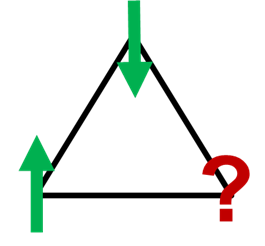
\includegraphics[width=0.2\columnwidth]{Chapter-1/geo_frustration.png} 
\protect\caption{\label{fig:intro-gf} An example of the geometric frustration in antiferromagnetic Ising model. There are more than one ground states even in this simple triangular lattice. A more complex network would lead to more frustrations.}
\end{figure}

Two main commonalities are geometric frustration and glassy dynamics  in these systems. First, the geometric frustration is introduced either by random interaction or complex structure \cite{vannimenus1977}. For example, in AFM, any odd loop in the structure can lead to the geometric frustration \cite{wannier1950afm} (as illustrated by Fig. \ref{fig:intro-gf}). In spin glass, the interaction constant $J_{ij}$ between spin $i$ and $j$ is random and can be either negative or positive, which is known as frustrated interaction \cite{edwards1975theory}.
Second, the glassy dynamics is often observed in the simulations of these disordered systems \cite{lunkenheimer2000}. For example, a strongly interacting glassy material is observed to have a power-law relaxation \cite{palmer1984}. These glassy dynamics often lead to the glass transition \cite{biroli2013perspective} or jamming transition \cite{Liu1998}. 
In all the three Chapters (Chapter 2 - 4), the disordered systems studied share both the geometric frustration and the glassy dynamics with a power-law relaxation, and we explore to see whether there is any phase transitions or glass transitions.

Another commonality is the analytical and computational complexity. Analytically, only certain models in certain lattices or structures are exactly solvable. For example, the mean field theory  \cite{kadanoff2009} is the most popular method to solve problems of spin glass \cite{sherrington1975}, lattice glass model \cite{Biroli02}, fully frustrated XY model \cite{kim2001xy}, etc. However, the majority of these models in real world lattice or complex networks are not analytically solvable. Moreover, their computational complexity is often NP-complete \cite{garey1983} because the computational cost grows exponentially with the system size \cite{barahona1982, weigt2000}.

In our studies, we have the same difficulties. In order to address these problems, we utilize a combination \cite{cheng2015jamming, ma2016prb} of real-world-like lattices, Monte Carlo methods, and analytical method RG using scientific computing languages (C/C++, Python) and modern computing tools (Mathematica, MATLAB). Our physical modeling, computational implementations, and results are described in details in Chapter 2-4.


\section{Jamming Transition}
\label{sec:jam_intro}
The first focus here is on the jamming systems \cite{Biroli2007}. Those systems undergo 
a jamming transition from a liquid-like to a solid-like state with extremely slow 
dynamics at a high packing density. The most interesting part in this 
disordered system is the physics near the jamming transition. 
The jamming transition, as discussed by Liu and
Nagel in 1998~\cite{Liu1998} has been the focus of
intense study~\cite{Biroli2007,Liu2010,Berthier2011}. 

A granular disordered system with increasing density can reach a jammed state at which a finite yield stress develops, or at least extremely long relaxation times
ensue, similar to the emerging sluggish behavior observed when the
viscosity of a cooled glassy liquid seemingly diverges. Thus, a jamming
transition may be induced in various ways, such as by increasing density,
decreasing temperature, or/and reducing shear stress~\cite{Liu2010}.
Below the jamming transition, the system stays in long-lived meta-stable
states, and its progression to its corresponding equilibrium state
entails an extremely slow, non-Debye relaxation~\cite{Hill1985, Ciamarra2010, van2010}.

Jamming transitions have been observed in various types of systems,
such as granular media~\cite{Majmudar2007}, molecular glasses~\cite{Parisi2010,Angelani2007},
colloids~\cite{Trappe2001}, emulsions~\cite{Zhang2005}, foams~\cite{Berthier2011,DaCruz2002},
etc~\cite{Liu2010,van2010}. These systems can behave like stiff solids
at a high density with low temperature and small perturbations. In
these transitional processes, the systems can self-organize their
own structure to avoid large fluctuations~\cite{Berthier2011} and
to reach a quasi-stable jammed state, characterized by an extremely
slow evolution to the unjammed equilibrium state. The properties of
those quasi-stable non-equilibrium states as well as their corresponding
equilibrium state is the main focus of our work in jamming. 


The properties of the jamming transition have been studied 
extensively~\cite{Biroli2007,Majmudar2007,Liu2010}, but we still lack an essential
understanding of the physics underlying the jammed state. Theoretical
progress has been much slower than the accumulation of experimental
discoveries. One of the reasons is the scarcity of theoretical microscopic
models to capture the complex jamming process~\cite{Krzakala2008,Jacquin2011}. 

In recent years, a lattice glass model proposed by Biroli and Mezard
(BM)~\cite{Biroli02} has been shown as a simple but adequate means
to study the jamming process. It is simple because the model follows
specific dynamical rules which are elementary to implement in both
simulations and analytical work. In distinction to kinetically constrained
models such as that due to Kob and Andersen~\cite{Kob93}, in which
particles are blocked from leaving a position unless certain neighborhood
conditions are satisfied, BM embeds geometric frustration merely by
preventing the neighborhood of any particles to consist of more than
$l$ other particles. Beyond that, it proceeds purely thermodynamically.
The phase diagram can be reduced to just one (or both) of two control
parameters, chemical potential and temperature. Either is sufficient
to reproduce a jamming transition which is similar to that observed
in off-lattice systems~\cite{Biroli02}. 

Using this model in a mean-field network 
(i.e., a regular random graph), Krzakala \textit{et al.} find
jammed states in Monte Carlo simulations and a genuine thermodynamical
phase transition (ideal glass transition) in its mean-field analytical
solutions~\cite{Krzakala2008}. In other words, the jammed state coincides
with an underlying equilibrium state that possesses a phase transition
to a glassy state. There is also other work trying to prove the similar idea using mean-field models \cite{Rivoire03,berthier2011theory, Parisi2010}. That raises the prospect that this equilibrium phase transition might be the reason for the onset of jamming. However, such a connection between phase transition and jamming transition is hard to ascertain for finite-dimensional lattice glasses. Our work (Chapter \ref{chap-jamming}) focuses on jamming in finite-dimensional hierarchical networks which could contribute closer insights to real world systems.



\section{Ising models}
The Ising model was proposed by Wilhelm Lenz and Ernst Ising \cite{ising1925contribution, brush1967history} in the 1920s. It has simple nearest-neighbor interactions and a simple Hamiltonian (energy)
\begin{equation}
\mathcal{H}=-J \sum_{\langle i, j\rangle}^N s_i s_j - H \sum_{i=1}^N s_i
\label{eq:intro-ising}
\end{equation}
where $s_i=\pm1$, $\langle i, j\rangle$ stands for nearest-neighbor spin-pair, $s_i$ $J$ ($>0$)is the exchange interaction constant, and $H$ is the external magnetic field. This is the most simple Ising model and usually called ferromagnetic Ising model (FM).
However, this simple model could represent approximately real-world systems and lead to phase transitions \cite{onsager1944} or complex dynamics \cite{Fredrickson1984} in different lattice structures. 
Numerous variations have been proposed to study different systems, ranging from magnetic systems \cite{blundell2001magnetism} to biological systems \cite{hopfield1982neural}.

In this section, two disordered Ising models, antiferromagnetic Ising model and random field Ising model,  are introduced and reviewed. They are also the focus the studies in Chapter \ref{chap-afm} and Chapter \ref{chap-rfim}.
\subsection{Antiferromagnetic Ising Model}
\label{sec:intro-afm}
Unlike ferromagnetic Ising model (FM) having a large amount of investigations, the antiferromagnetic Ising model (AFM) have little work published until 1970s \cite{penney2003new}. The most interesting characteristic of the AFM is that it can easily introduce geometric frustrations and may give rise to a glassy dynamics or even spin glass phase. While this interesting characteristic is realized by only change the the sign of the coupling constant $J$ ($J<0$), and the Hamiltonian is still the same as Eq. \ref{eq:intro-ising}.



\subsection{Random Field Ising Model}
\label{sec:intro-rfim}
The random field Ising model (RFIM) was first introcuded by Imry and Ma \cite{imry1975random} in 1975. It represents a class of quenched disordered spin models \cite{young1997spin} with  disorderness coupled to the each spin, which is different from the spin glass models with disordered interaction constants. The general Hamiltonian of RFIM with $N$ spins is
\begin{equation}
\mathcal{H}=-J\sum_{<i,j>}s_{i}s_{j}-\sum_{i=1}^{N}h_{i}s_{i}
\end{equation}
where the major difference from traditional Ising model is the random field term $h_i$ for spin $i$. Different spins usually have  identical independent distributed random fields $h_i$, and $h_i$ often follows a uniform \cite{nattermann1997theory} or Gaussian distribution \cite{newman1999}.

As a statistical mechanical model, the most investigated theoretical aspect of RFIM is still the critical phenomena, such as ferromagnetic phase transition. For one dimensional RFIM, its exact solution suggests no phase transition \cite{grinstein1983exact}. Through a number of theoretical calculations \cite{parisi1979random, bricmont1987lower}, three dimensional RFIM has a phase transition from a paramagnetic phase to a ferromagnetic one  \cite{bricmont1987lower}, which suggests the lower critical dimension is $d_l = 3$. 

However, the focus of our study in Chapter \ref{chap-rfim} is not the phase transition but the aging dynamics of the RFIM simulating experimental system. In terms of experimental studies, the diluted antiferromagnet is considered as an experimental realization of the RFIM \cite{belanger1985, fernandez1988random}. It has also been used to study other materials, such as  impure substrates \cite{villain1982commensurate}, and magnetic alloys \cite{fisher1988theory}. 
The experimental system to model here is a thin-film ferromagnet/antiferromagnet bilayer which exhibits non-Arrhenius power-law aging of the magnetization state \cite{ma2016prb}. 
It is expected that, in such a complex experimental magnetic system, the aging or relaxation to equilibrium state may be trapped by metastable states, and the relaxation may follow an exponential scaling according to the Arrhenius law \cite{Arrhenius1989}
\begin{equation}
\tau = \tau_0 \exp \left( \frac{E}{k_B T}\right)
\end{equation}
where $\tau$ is the characteristic activation time, $\tau_0$ is a material-dependent pre-exponential factor, $E$ is the energy barrier between two local/local (or local/global) minimum, $k_B$ is the Boltzmann constant, and $T$ is the temperature. However, what is observed in the experiment is a power-law relaxation with a subunity exponent instead of exponential relaxation. The experiment itself cannot explain this phenomena, and the small exponent is not convincing either to conclude the power-law relaxation. 

In order to explain the experiment and justify the small-exponent power-law, we use a two dimensional RFIM and the Monte Carlo method to simulate the experimental material with simplifying approximations. This simple model captures the salient features of the non-Arrhenius aging observed in the experimental measures, i.e., power-law relaxation with a subunity exponent. In addition to the scaling, the aging in the Monte Carlo simulation can be easily visualized, which shows the system evolves to two big domains with oppositely oriented spins. What the aging can do is actually smoothing the domain wall between these two domains, and the system can never break the barrier imposed by the domain wall. More details are described in Chapter \ref{chap-rfim}.

\section{Hanoi Networks}
\label{sec:HN} 
In our investigations, one of the innovative insights is contributed from the finite-dimensional lattice-like networks. We use 4 types of Hanoi networks ~\cite{Boettcher2008HN} which are small-world networks with a hierarchical, recursive structure that avoid the usual randomness involved in defining
an ensemble of networks. Thus, no additional averages of such an ensemble
are required to obtain scaling properties in thermodynamical limit
from a finite system size, which reduces the computational effort.
Hanoi networks combine a real-world geometry with a hierarchy of small-world
links, as an instructive intermediary between mean-field and finite-dimensional
lattice systems, on which potentially exact results can be found using
the renormalization group~\cite{BoHa11}. 

\begin{table}
\begin{centering}
\protect\caption{\label{tab:hns} 
Summary of Hanoi networks at system size $N\rightarrow\infty$ }
\par\end{centering}
\begin{centering}
\par\end{centering}
\centering{}%
\begin{tabular}{|c|c|c|c|c|}
\hline 
Network & Degree  & Planarity & Diameter & Fractal Dimension  \tabularnewline
\hline 
\hline 
HN3  & $3$ & Planar & $\sqrt{N}$ & 2 \tabularnewline
\hline 
HN5  & $5$ & Planar &  $\ln N$ & $\infty$  \tabularnewline
\hline 
HNNP  & $4$  & Nonplanar &  $\ln N$ & -  \tabularnewline
\hline 
HNNP  & $6$  & Nonplanar &  $\ln N$ & - \tabularnewline
\hline 
\end{tabular}
\end{table}

Across all the chapters, we use four Hanoi networks (HNs): HN3, HN5, HNNP, and HN6. Their general characteristics are summarized in Table \ref{tab:hns}. These HNs have different degrees, planarities, diameters, and fractal dimensions, each of which may have different effects on the model. For example, there have been studies showing different degrees of connections may affect the critical phenomena \cite{dorogovtsev2008critical, herrero2002ising}; the planarity of complex networks may affect Ising model's phase transition \cite{fisher1966dimer, istrail2000statistical} and computational complexity \cite{barahona1982}.


Each of them can be built on
a simple backbone of a 1D lattice. The 1D backbone has $N=2^{k}+1$
($k=1,2,3,\cdots$) sites where each site is numbered from $0$ to
$N$. Any site $n$, $0\le n\le N$, can be defined by two unique
integers $i$ and $j$, 
\begin{equation}
n(i,j)=2^{i-1}(2j+1),\label{eq:numbering}
\end{equation}
where $i$, $1\le i\le k$, denotes the level in the hierarchy and
$j$, $0\le j<2^{k-i}$, labels consecutive sites within each
hierarchy $i$. Site $n=0$ is defined in the highest level $k$ or,
equivalently, is identified with site $n=N$ for periodic boundary
conditions. With this setup, we have a 1D backbone of degree
2 for each site and a well-defined hierarchy on which we can build
long-range links recursively in three different ways: HN3~\cite{Boettcher2008HN}
is constructed by connecting the neighbor sites $n(i,0)\longleftrightarrow n(i,1)$,
$n(i,2)\longleftrightarrow n(i,3)$, $n(i,4)\longleftrightarrow n(i,5)$,
and so on and so forth. For example, in level $i=1$, site $n(1,0)=1$
is connected to $n(1,1)=3$; site $n(1,2)=5$ is connected to $n(1,3)=7$;
and so on. A initial section of a HN3 network is given in Fig.~\ref{fig:HN3_short}.
As a result, HN3 is a planar network of regular degree 3.

\begin{figure}
\centering 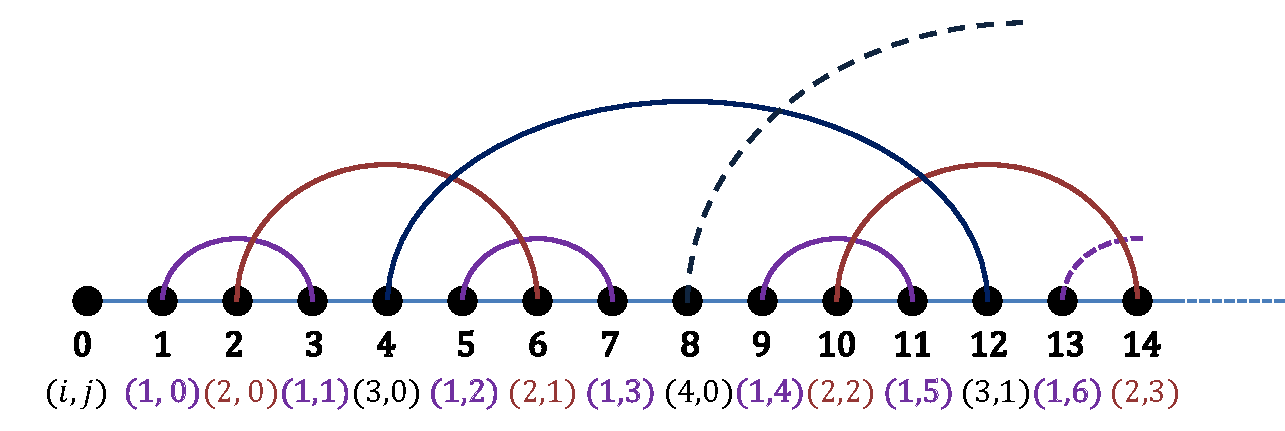
\includegraphics[width=1\columnwidth]{Chapter-1/HN3_short.pdf} 
\protect\caption{\label{fig:HN3_short} An example of the first 14 sites of HN3 on a semi-infinite line.}
\end{figure}


HN5~\cite{Boettcher09c}, as shown in Fig.~\ref{fig:Depiction-of-HN},
is an extension based on HN3, where each site in level $i$ ($i\ge2$,
i.e., all even sites) is further connected to sites that are $2^{i-1}$
sites away in both directions. For example, for the level $i=2$ sites
(sites $2,6,10,\cdots$), site 2 is connected to both site 0 and site
4; site 6 is connected to sites 4 and 8; etc. The resulting network
remains planar but has a hierarchy-dependent degree, i.e., 1/2 sites
have degree 3, 1/4 have degree 5, 1/8 have degree 7, etc. In the limit
of $N\to\infty$, this network has  average degree 5.

\begin{figure}
\centering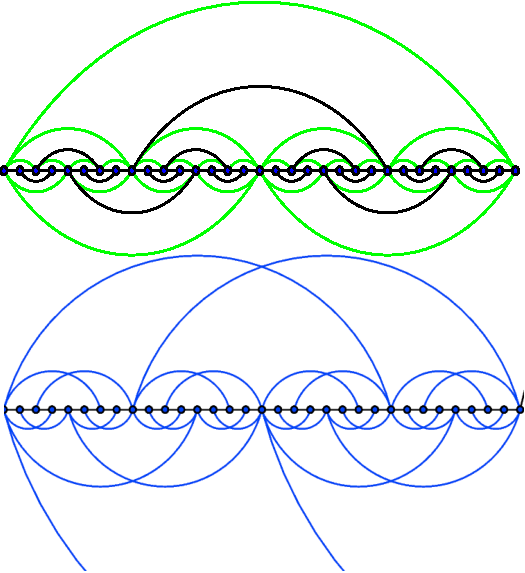
\includegraphics[width=0.8\columnwidth]{Chapter-1/HN5HNNP}
\protect\caption{\label{fig:Depiction-of-HN}Depiction of HN5 (top) and HNNP (bottom),
first introduced in Ref. \protect\cite{Boettcher09c}. Green-shaded lines
in HN5 represent its difference to HN3, which is at its core (dark
lines). While HN3 and HN5 are planar, HNNP is non-planar. }
\end{figure}

HNNP~\cite{Boettcher09c}, also shown in Fig.~\ref{fig:Depiction-of-HN},
is constructed from the same 1D backbone as HN3 and HN5. However,
for site $n$ in level $i$ with even $j$, it is connected forwards
to site $(n+3\times2^{i-1})$; while site $n$ in level $i$ with
odd $j$ is connected backwards to site $(n-3\times2^{i-1})$. Level
1 and level 2 sites have degree 3, and level $3,4,5,\cdots$ sites
have degree $5,7,9,\cdots$. The HNNP has an average degree of 4 and
is non-planar.

HN6 \cite{Boettcher09c} is constructed from HNNP in the same way of constructing HN5 from HN3. The extra links are initiated from site in level $i$ ($i\ge2$ who
i.e., all even sites)  connects to sites that are $2^{i-1}$
sites away in both directions. The resulting network is still a nonplanar with hierarchy-dependent degree.

As you can see, these four networks are all constructed hierarchically and can potentially use renormalization group in a similar way. Using these networks, renormalization group has been applied to lattice gas model \cite{cheng2015jamming, BoHa11} and ferromagnetic Ising model \cite{Boettcher2011HNNP, boettcher2015classification}. In the study here, the models are extended to lattice glass model and antiferromagnetic Ising model. 




\section{Computational Methods}
In all the three projects in this dissertation, the computational methods are the most important part to implement the models and realize the computations. We use a wide range of different computational methods, such as Markov-Chain Monte Carlo (MCMC) method, non-Markov-Chain Monte Carlo method, Renormalization Group (RG), numerical analysis, and graphical models.
 These methods requires a broad knowledge in computer science, physics, mathematics, and statistics. Moreover, their implementations take a large amount of time and effort for coding,  testing, computation, and analysis. Our computational work may not only contribute new insights in physics but also shed light onto algorithms development and optimizations.

Specifically, we mainly adapted and implemented three advanced methods: Simulated Annealing (SA), Wang-Landau sampling (WL), and Renormalization Group (RG). 

The Simulated Annealing (SA) \cite{SA} was first formulated as an approach to find a minimization of a function with a large number of variables in statistical mechanics \cite{khachaturyan1979statistical, khachaturyan1981thermodynamic}. This algorithm imitates the slow cooling process in metallurgy to increase its crystallization and reduce its defects. In the implementation of the algorithm, it slowly decrease the probability of accepting worse transitions or solutions to robustly find a local or global minimum. In physics, the probability of a worse transition is usually controlled by the temperature, which makes this name self-explaining. Kirkpatrick {\it et. al.} \cite{SA} published a famous paper on {\it Science} to formally define, apply, and discuss SA  in the scenarios of combinatorial optimization, statistical mechanics, physics design of computer, and even the famous traveling salesmen's problem. It is a widely used method not only to search for a global minimum but can also to simulate the dynamics of a physical system because the annealing process simulates the physical process.
In the implementation of SA in our studies, our goal is not only simply search for the minimum (ground states) but also learn the relaxation dynamics. This process is extremely costly in terms of the computational time because we need to cool the system slowly and repeat the annealing many times ($50\sim 1000$ runs in our projects). For most SA results in Chapter 2 and 3, each curve takes about $\sim ~50$ hours using sequential computation on a single core. More detailed computing setup is described in the chapters using SA.


The Wang-Landau sampling (WL) \cite{Wang2001} is a computational methods using non-Markov-chain Monte Carlo; while RG is an analytical methods but requires the computational implementation using modern symbolic computational tools (Mathematica).


The Renormalization Group (RG) is an analytical method to take advantage of the symmetries in the problem and renormalize the problem to a low-dimensional one. 












\chapter{Jamming in Hanoi Networks}
\label{chap-jamming}

In this chapter \footnote{The results of this chapter have been published in Ref. \cite{cheng2015jamming}.}, we propose to use the lattice glass model (BM model) on hierarchical
networks~\cite{Boettcher2008HN}, which are networks with a fixed,
lattice-like geometry. They combine a finite-dimensional lattice backbone
with a hierarchy of small-world links that in themselves impose a
high degree of geometric frustration despite of their regular pattern.
In fact, the recursive nature of the pattern can ultimately provide
analytical solution via the renormalization group (RG), positioning
these networks as sufficiently simple to solve as well as sufficiently
lattice-like to become an alternative to mean-field solutions~\cite{BoHa11}. 
Unlike mean-field models, our network is dominated by many small loops that are also the hallmark of lattice systems. Our goal is to find 
\begin{enumerate}
\item whether the lattice glass model leads to jamming
state in hierarchical networks;
\item whether there is an ideal glass
transition underlying the jamming transition;
\item whether the local dynamics affect the jamming process. 
\end{enumerate}
To our knowledge, these questions have not been studied in any small-world systems. Our results can contribute new insights to understand jamming.

We find that BM in these networks can jam, even when there is certifiably
no equilibrium transition; the geometric frustration that derives
from the incommensurability among the small-world links is sufficient
in many cases to affect jamming. In fact, jamming is most pronounced
for fully exclusive neighborhoods ($l=0$). It disappears for more
disordered neighborhoods ($l=1$), at least for our non-regular networks,
where the allowance of $l=1$ neighbor to be occupied seems to provide
the ``lubrication'' that averts jams. However, the packing fractions
at which time-scales diverge is virtually indistinguishable from random
close packing within the accuracy of our simulations. 

Mean-field calculations of BM in Ref.~\cite{Rivoire03} predict a kinetic transition for dynamic rules based on nearest-neighbor hopping. In our simulations, we find that  such hopping,  in addition to the particle exchange with a bath, can affect a dramatic change in the dynamic behavior and eliminated jamming in all cases we consider.  

%This chapter is organized as follows. In Sec.~\ref{sec:jam_model}, we describe
%the lattice glass model. Then we describe in detail  how we implement 2 Monte Carlo methods in Sec. ~\ref{sec:jam_methods}. The results of our simulations is discuss in Sec. ~\ref{sec:jam_results}. In Sec. \ref{sec:jam_conclusions} we conclude with a few summary remarks and an outlook for future work.


\section{Lattice glass model}
\label{sec:jam_model}

The lattice glass model as defined by
Biroli and Mezard (BM)~\cite{Biroli02} considers a system of particles
on a lattice of $N$ sites. Each site can carry either $x_{i}=0$
or $x_{i}=1$ particle, and the occupation is restricted by a hard,
local ``density constraint'': any occupied site ($x_{i}=1$) can
have at most $l$ occupied neighbors, where $l$ could range locally
from 0 to the total number of its neighbor-sites. In this model, the
jamming is defined thermodynamically by rejecting the configurations
violating the density constraint. Here, we focus on global density
constraints of $l=0$ (completely excluded neighborhood occupation)
and $l=1$ as the most generic cases. The system can be described
by the grand canonical partition function 
\begin{equation}
Z(\mu)=\sum_{{\bf allowed}\,\{x_{i}\}}\exp\left[\mu\sum_{i=1}^{N}x_{i}\right],\label{eq:PF}
\end{equation}
where the sum is over all the allowed configurations $\{x_{i}\}$.
Here, $\mu$ is the reduced chemical potential, where we have chosen
units such that the temperature is $k_{B}T=1/\beta=1$, and $\sum_{i=1}^{N}x_{i}$
is the total number of particles in a specific configuration.

From the grand canonical partition function in Eq.~(\ref{eq:PF}),
we can obtain the thermodynamic observables we intend to measure,
such as the Landau free energy density $w(\mu)$, the packing fraction
$\rho(\mu)$, and the entropy density $s\left[\rho(\mu)\right]$,
as defined in the following equations:
\begin{eqnarray}
w(\mu) & = & -\frac{1}{N}\ln Z,\label{eq:GCPdiff}\\
\rho(\mu) & = & \frac{1}{N}\left<\sum_{i=1}^{N}x_{i}\right>_{\mu}=\frac{1}{N}\frac{\partial\ln Z}{\partial\mu},\nonumber \\
s(\mu) & = & \frac{1}{N}\left(1-\mu\frac{\partial}{\partial\mu}\right)\ln Z.\nonumber 
\end{eqnarray}
 
\section{Monte Carlo Methods}
\label{sec:jam_methods} 

We aim to learn both the non-equilibrium dynamics and equilibrium behaviors in our model and networks. To benchmark the equilibrium properties of the model on those networks, we implement a multi-canonical algorithm due to Wang and Landau~\cite{Wang2001, wang01a}. We further need a grand-canonical annealing algorithm to study the dynamics of the
lattice glass model on those networks.

\subsection{Wang-Landau Sampling}
\label{sub:WLsampling}Wang-Landau sampling~\cite{Wang2001} is a
multi-canonical method to numerically determine the entire density
of states $g_{n}$ within a single simulation. This method is initially proposed to study 
ferromagnetic Ising model, and we independently modify this algorithm to sample  
density of states in the lattice glass model.
 
As introduced in Sec. \ref{sec:intro-comp}, this method is based on 
the fact that a random walk in the configuration space with a probability
proportional to the inverse of the density of states with occupation
$n$, $0\leq n\leq N$, enforces a flat histogram in $g_{n}$ over
all $n$. Based on this fact, Wang-Landau sampling keeps modifying
the estimated density of states in the random walks over all possible
configurations and can make the density of states converge to the
true value. The sampling procedure is: 
\begin{enumerate}
\item Initially, set all unknown density of states $\{g_{n}=1\}$ and the
histogram $\{H_{n}=0\}$ for all occupations $n$, initiate the modification
factor $f=e^1\approx2.71828\dots$ ; 
\item Randomly pick a site $i$; if it is empty (occupied), add (remove)
a particle with a probability of $\min\left[1,\frac{g_{n}}{g_{n+1}}\right]$
($\min\left[1,\frac{g_{n}}{g_{n-1}}\right]$) while obeying the rule
of the hard local density constraint on having at most $l$ occupied
nearest neighbors of site $i$; 
\item Randomly pick one occupied site and one empty site; transfer
a particle from the occupied site to the empty, if the density constraint is not violated; 
\item Update the $H_{n}$ and $g_{n}$ of the current state, i.e., set $\{H_{n}=H_{n}+1\}$
and $\{g_{n}=g_{n}\times f\}$; 
\item Repeat steps 2 to 4 until the sampling reaches a nearly flat histogram
for the $H_{n}$, then update the modification factor $f=\sqrt{f}$
and reset $\{H_{n}=0\}$; 
\item Stop if $f\le1+10^{-8}$. 
\end{enumerate}
Our procedure mostly follows the standard procedure of Wang-Landau
sampling~\cite{Wang2001}, except for step 3. Its purpose is to facilitate
the random walk to explore phase space more broadly and to expedite
convergence.

Wang-Landau sampling has been proved as an effective method to find
the density of states~\cite{Wang2001,Lee2006,Dickman2011}. In our
study, it can find convergence for system size of up to $N\sim10^{3}$
within a reasonably computational cost. From the density of states,
we can calculate the equilibrium thermodynamical properties for the
corresponding system sizes. 


\subsection{Grand-Canonical Annealing}

\label{sub:GCannealing} In parallel to the equilibrium properties
provided by Wang-Landau sampling, we also implement a form of simulated
annealing~\cite{SA} to explore the dynamics of the model and the
possibility of jamming, in a process that is similar to an experiment.
Simulated annealing used in this study follows the standard procedure
~\cite{Vcerny1985}. The corresponding experiment is exchanging particles
between the network and a reservoir of particles with (dimensionless)
chemical potential $\mu$. In our study, the annealing speed is not
controlled by decreasing temperature (which we set to $\beta=1$)
but by increasing the chemical potential. The procedure of the annealing algorithm
is: 
\begin{enumerate}
\item Initially, start with chemical potential $\mu_{0}=0$ ; 
\item Randomly pick a site $n$; if it is empty (occupied), add (remove)
a particle with a probability of $\min\left[1,\exp(\mu)\right]$ ($\min\left[1,\exp(-\mu)\right]$)
while obeying the rule of the hard local density constraint on having
at most $l$ occupied nearest neighbors of $n$; 
\item If hopping is allowed, randomly pick one site; only if it is occupied,
randomly pick one of its empty neighbor(s) and displace the particle
if the density constraint remains satisfied; 
\item Increase $\mu$ by $d\mu$ every 1 Monte Carlo sweep ($N$ random
updates), where $d\mu/dt$ (in time-units of $dt=1$) is the annealing
schedule and $d\mu\ll1$; 
\item Repeat steps 2 to 4 until $\mu$ reaches a certain (large) chemical
potential. 
\end{enumerate}
Following the procedure above, the simulated annealing can reveal
whether or not a jamming transition occurs in the process. Besides
that, we can test the effect of local dynamics~\cite{Biroli02, Krzakala2008}
by adding a local hopping random walk (step 3), i.e., a particle can
transfer any of its empty neighboring sites as long as 
the constraint remains satisfied.  The results are shown and explained in
the following section.


\section{Results}
\label{sec:jam_results} 
To assess the properties of jamming, we first
have to benchmark our systems with the corresponding equilibrium behaviors.
After that, we discuss the dynamic simulations with the annealing
algorithm in reference to these equilibrium benchmarks.


\subsection{Equilibrium Properties\label{sub:Equilibrium-PropertiesWang-Landa}}

Wang-Landau sampling, as described in Sec.~\ref{sub:WLsampling},
is ideally suited for our purpose, since it provides access directly
to the density of states $g_{n}$ as a function of occupation number
$n$, which yields the partition function as
\begin{equation}
Z(\mu)=\sum_{n=0}^{n_{max}}g_{n}e^{n\mu}.\label{eq:Zmu}
\end{equation}
All thermodynamic quantities in the equilibrium can be obtained numerically
by summation of the formal derivates of $Z(\mu)$, such as those in
Eqs.~(\ref{eq:GCPdiff}), over all permissible occupation numbers
$0\leq n\leq n_{max}<N$. (For all $n_{max}<n\leq N$ it is $g_{n}=0$.) 


\begin{table}
\begin{centering}
\protect\caption{\label{tab:cpf} Closest packing fractions $\rho_{CP}$ found by Wang-Landau sampling. The values for $l=0$ have been previously obtained with exact RG,
the one for HNNP being unique, with every second, odd site occupied.
For $l=1$, we also predict exact fractions with nontrivial entropy
densities, see Fig.~\ref{fig:doswl}. However, the results for $l=1$ is based on results of system sizes $16\le N \le 512$. The closest packing fraction may change for larger system sizes.}
\par\end{centering}
\begin{centering}
\par\end{centering}
\centering{}%
\begin{tabular}{|c|c||c|}
\hline 
Network & $l=0$  & $l=1$ \tabularnewline
\hline 
\hline 
HN3  & 3/8~\cite{BoHa11} & 9/16 \tabularnewline
\hline 
HN5  & 1/3~\cite{BoHa11} & 1/2 \tabularnewline
\hline 
HNNP  & 1/2  & 1/2 \tabularnewline
\hline 
\end{tabular}
\end{table}


\begin{figure}[h]
\centering 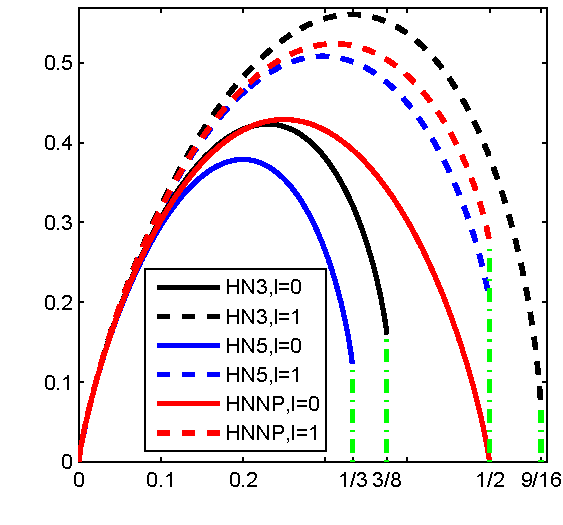
\includegraphics[width=0.6\columnwidth]{Chapter-2/Paper_DOS_Plot2}
\protect\caption{Density of states from Wang-Landau sampling at $N=1024$. The green
dash-dot vertical line are showing the closest packing fractions (as
shown in Table \ref{tab:cpf}) for each system. Note that only for
HNNP at $l=0$ there is a unique, crystalline ground state. }
\label{fig:doswl} 
\end{figure}

In Fig.~\ref{fig:doswl}, we plot the density of states as a function
of the packing fraction, both obtained with Wang-Landau. It becomes
apparent that each model has a simple rational value for its optimal
($\mu\to\infty$) ``random'' close packing fraction $\rho_{CP}=n_{max}/N$.
This corresponds to a random packing in the sense that it has a nontrivial
entropy density due to geometric disorder (imposed by the lack of
translational invariance in the lattice), except for HNNP at $l=0$,
which has a unique ``crystalline'' packing of every odd site being
occupied. While these values for $\rho_{CP}$ have been previously
obtained with RG for $l=0$~\cite{BoHa11}, the simulations predict
also strikingly simple but nontrivial values for $l=1$, where exact
RG is likely not possible. These values are listed in Table \ref{tab:cpf}.


\begin{figure}
\centering 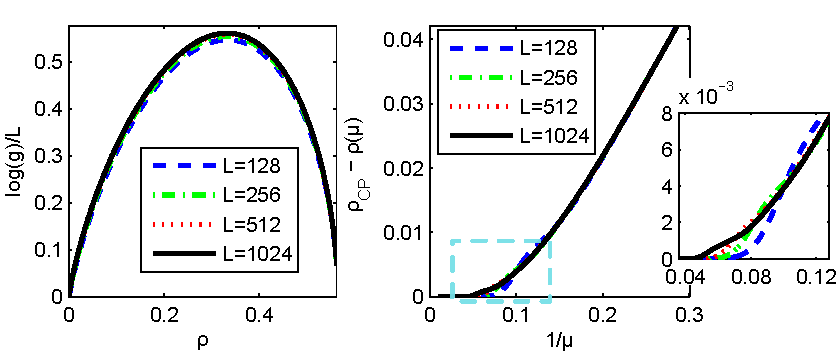
\includegraphics[width=1\columnwidth]{Chapter-2/Paper_ConvergenceHN3_Plot2}
\protect\caption{Convergence to the thermodynamic limit for finite system sizes for
the example of HN3 with $l=1$ using Wang-Landau sampling. The figures are
for the density of states (left) and the packing fraction (right). The
equilibrium packing fraction $\rho(\mu)$ as a function of chemical
potential $\mu$ is calculated from the density of states according
to Eq.~(\ref{eq:GCPdiff}); it approaches the closest packing fraction
$\rho_{CP}$ for $1/\mu\to0$. The convergence for other systems is
similar or better. }
\label{fig:WLconverge} 
\end{figure}


\begin{figure}[h]
\centering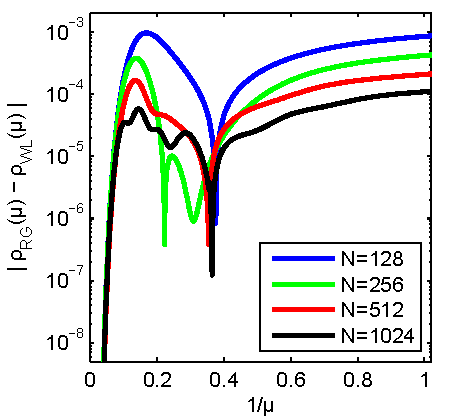
\includegraphics[width=0.6\columnwidth]{Chapter-2/Paper_HN3_l0_RGvsWL_error-eps-converted-to}\protect\caption{\label{fig:RGvsWL} 
Plot of the error in the finite-size packing fraction
in Wang-Landau sampling, $\left|\rho_{WL}-\rho_{RG}\right|$, as a
function of $1/\mu$ near close packing ($\mu\to\infty$) in HN3 at
$l=0$. Here, RG result $\rho_{RG}(\mu)$ from Ref. \protect\cite{BoHa11}
at system size $N=2^{500}$ is taken as the exact, thermodynamic packing
fraction. Relative to $\rho_{RG}(\mu)$, the finite-size packing fraction,
$\rho_{WL}(\mu)$, at $N=2^{k}$ with $k=8,9,10$ already exhibit
quite small and rapidly diminishing corrections. }
\end{figure}


Wang-Landau sampling converges within a reasonable time for system
sizes smaller than $N\approx2000$ but fails to converge for larger
system size within ~2 weeks of computational time. 
There may be two reasons for the lack of convergence:
(1) the density of states is not symmetric as a function of packing
fraction, and this asymmetry requires Wang-Landau to sample the whole
configuration space, which increases the computational cost dramatically
especially for large system sizes; (2) the lower the density of states
of the closest packed state, the harder it is for Monte Carlo sampling
to find its closest packing state because of the hard density constraint.
Although Wang-Landau sampling fails for large system sizes, the results
of system size $N=1024$ can still offer an insight to the equilibrium
state because the density of states and the packing fraction exhibit only small 
finite-size corrections for increasing $N$. For example, the convergence of HN3
with $l=0$ is shown in Fig.\ref{fig:WLconverge}. Other networks
with $l=0,1$ have similar or even better convergence.

We can further demonstrate the quality of the Wang-Landau simulations,
and appraise their residual finite-size effects, by comparison with
exact results obtained with the renormalization group (RG) for $l=0$
on HN3~\cite{BoHa11}. In Fig.~\ref{fig:RGvsWL}, we compare the results
for the packing fraction $\rho(\mu)$ as a function of the chemical
potential for Wang-Landau sampling on networks with $N=2^{k}$ sites, $k=8\sim10$,
with those from the exact RG after 500 iterations, corresponding
to a system of $N=2^{500}$ sites. Despite the much smaller sizes
of the Wang-Landau simulation, its results are barely distinguishable
from the exact result, affirming the Wang-Landau sampling results
as good references for our dynamic simulations, with negligible finite-size
effects.


\subsection{Dynamic Properties}

\label{subsec:jamsc} The dynamic simulations of the BM on our networks
uses the grand canonical partition function controlled by a chemical
potential $\mu$ that mimics the experimental situation in a complex
fluid or colloid, where particles are pumped into the larger system
(the reservoir) and can enter the field-of-view through open boundaries
inside a smaller window. For example, this could correspond to a $2d$
slice of a $3d$ colloidal bath used in colloidal tracking experiments
~\cite{Hunter12}. Since our particles are not energetically coupled
and merely obey hard excluded volume constraints, temperature is irrelevant
and we can set $\beta=1$, making the chemical potential dimensionless,
$\beta\mu\to\mu$. As we increase $\mu$, the system is more likely
to accept more particles and increase the packing fraction $\rho(\mu)$.
When $\mu$ is small (or negative), the reservoir and the network
readily reach an equilibrium state with a certain packing fraction.
However, when $\mu$ is large, the equilibrium state defined by the
partition function has a packing fraction close to the close packing
$\rho_{CP}$. Because of the density constraint and the disorder imposed
by the hierarchical network geometry, the system enters into a jam
at a density far from equilibrium packing. As in experiments, this
jammed state remains for an extremely long time, even when $\mu$
is further increased. The ultimate packing fraction $\rho^{*}$ that
the systems gets stuck at, in fact, is ever further from random close
packing, the faster the quench in $\mu$ is executed, where $\frac{d\mu}{dt}$
is the quench rate. In this, our results closely resemble those reported
in Ref.~\cite{Krzakala2008}. 

\begin{figure}
\centering 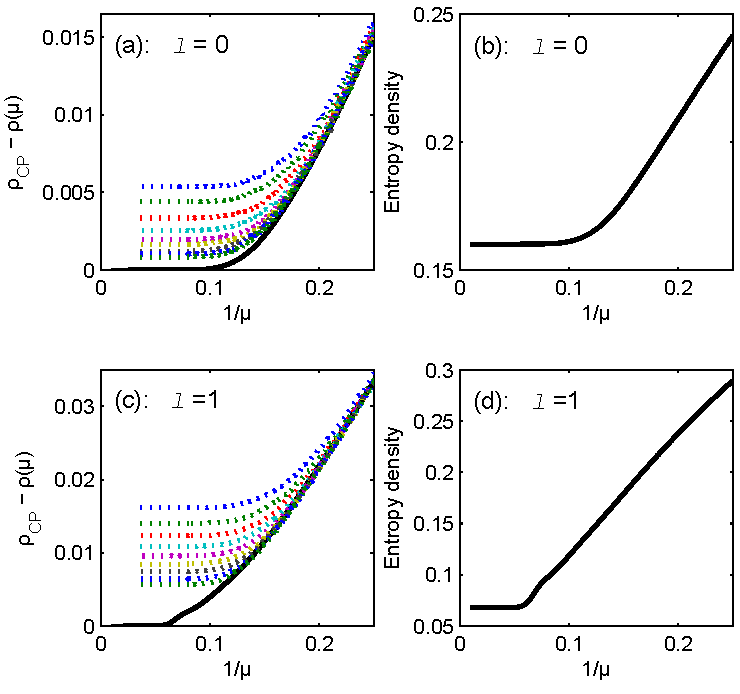
\includegraphics[width=1\columnwidth]{Chapter-2/Paper_HN3_PackMu_Entropy_l01_Plot}
\protect\caption{Reduced packing fraction and entropy density for HN3 from Wang-Landau
sampling and Simulated Annealing. (a)\&(b) are for $l=0$, and (c)
\&(d) are for $l=1$. The black solid lines represent the equilibrium
properties from Wang-Landau sampling with $N=1024$. The dotted lines
are from simulated annealing with $N=32,768$, run at different annealing
schedules with $d\mu=0.001/2^{j}$ for $j=0,\ldots,8$, from top to
bottom. Wang-Landau sampling provides the entropy density via Eq.
(\ref{eq:GCPdiff}), as shown in (b) and (d), which is difficult to
obtain from other Monte Carlo methods. For both, $l=0$ and 1, we
find a non-zero entropy density for random close packing at $\mu\rightarrow\infty$.}
\label{fig:HN3PE} 
\end{figure}


\begin{figure}
\centering 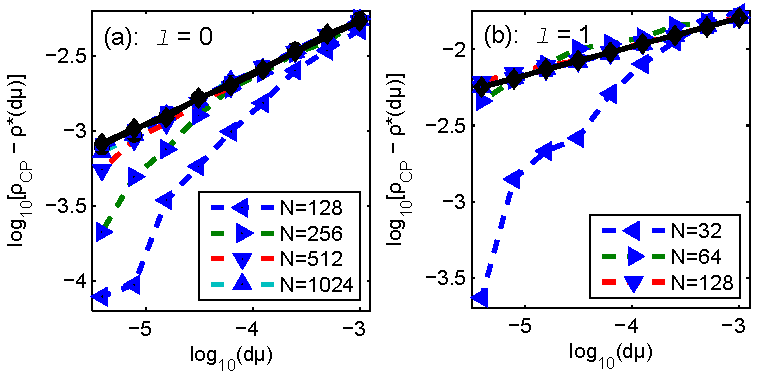
\includegraphics[width=0.9\columnwidth]{Chapter-2/Paper_HN3_Decay}
\protect\caption{Scaling of the dynamically reached packing fraction $\rho^{*}(d\mu)$
as a function of the annealing rate $d\mu$ for different system sizes
$N$ of HN3. (a) For $l=0$, the dashed lines are for systems sizes
$N=2^{k}$ with $k=7,\ldots,$10, 12, 14 and 15, from bottom to top.
All data sets (except for the smallest sizes, $N=128,\ldots,1024$)
collapse onto the top line with a slope of $0.34\pm0.01$, which is
obtained from a fit using the data of the largest system size $N=32,768$.
(b) For $l=1$, the data sets converge even faster towards power-law
scaling. The dashed lines are for system sizes of $N=2^{k}$ with
$k=5,\ldots,8$, 10, 12, 14 and 15, from bottom to top. All but the
first 3 sets collapse onto a line of slope $0.19\pm0.01,$ which is
obtained from a fit for $N=32,768$. Error bars are about of the size
of each data point or smaller, indicating a relative error of less
than $3\%$.}
\label{fig:HN3Decay} 
\end{figure}


\begin{figure}
\centering 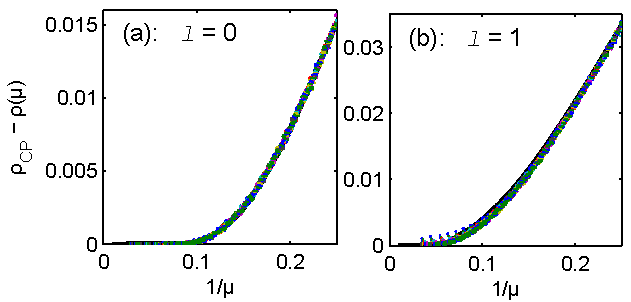
\includegraphics[width=0.9\columnwidth]{Chapter-2/Paper_HN3_Hopping_Plot}
\protect\caption{\label{fig:HN3hopping} 
Results of simulated annealing with hopping for HN3. For both (a)
and (b), the figure consists of one solid line for the equilibrium
result obtained with Wang-Landau sampling and 9 dotted lines obtained
with simulated annealing at rates $d\mu=0.001/2^{j}$ for $j=0,\ldots,8$.
For HN3 with $l=0$ and $l=1$, the system equilibrates for nearly
all annealing schedules, collapsing the data onto the equilibrium
line. Only for HN3 with $l=1$, small deviations from equilibrium
are observed for annealing schedules $d\mu \le10^{-5}$. } 
\end{figure}



\subsubsection{Results for HN3}

\label{subsec:HN3}

The equilibrium packing fraction and entropy from Wang-Landau sampling
as well as the dynamic results from simulated annealing for HN3 are
shown in Fig.~\ref{fig:HN3PE}. Based on the analytical results by
Boettcher \textit{et al.}~\cite{BoHa11}, we can confidently conclude
that there is no phase transition in HN3 with $l=0$. Yet, the dynamic
simulations indicate that the system jams nonetheless. The system
jams even further from equilibrium for the case of $l=1$. Here, RG
results have not been obtained so far and it is not clear whether
there is a thermodynamic phase transition. The equilibrium results
from Wang-Landau sampling (at $N=2^{10}$) seem to suggest a singularity
near $1/\mu\approx0.06$ where the entropy density jumps noticeably
and $\rho(\mu)\equiv\rho_{CP}$ for all larger $\mu$. Either RG or
results for bigger systems may be needed to confirm whether there
is phase transition or not. 

The possible jamming transitions for both $l=0$ and $1$, revealed
by the dynamic annealing simulations in Fig.~\ref{fig:HN3PE} (a)
and (c), are further supported by a power law decay of the residual
packing fractions, $\rho_{CP}-\rho^{*}(d\mu)$, as a function of the
annealing rate, $d\mu$. Here, we set the jammed packing fraction,
obtained at $\mu\to\infty$ after annealing at rate $d\mu$, as $\rho^{*}(d\mu)=\rho(\mu\to\infty;d\mu)$,
where $d\mu/dt\to d\mu$ when measured in units of $dt\hat{=}1$ sweep.
Note that at these system sizes ($N=32,768$), even the weakest jam
is of order $\rho_{CP}-\rho^{*}(d\mu)\approx0.001$ and, thus, still
consists of a sizable number ($ > 30$) of frustrated particles. 

As shown in Fig.~\ref{fig:HN3Decay}, a linear fit of the data on
a double-logarithmic scale at the largest systems  is
nearly perfect, justifying the assumption that the time-scales $1/d\mu$
for the existence of the jam diverge asymptotically with a power law
for $\rho\to\rho_{CP}$. For HN3 at $l=0$, the slope is $0.34\pm0.01$
with coefficient of determination $R^{2}=0.9975$, while for $l=1$
the slope is $0.19\pm0.01$ with $R^{2}=0.9997$, in both cases indicating
a dramatic increase of time-scales. 

We also test the effect of introducing local hopping, implemented
as suggested in step 3 of the algorithm in Sec.~\ref{sub:GCannealing},
which has not been addressed in Refs.~\cite{Krzakala2008, Biroli02}.
The results shown in Fig.~\ref{fig:HN3hopping} indicate a substantial
difference from the simulation without hopping. For HN3 with $l=0$,
the jamming transition disappears even for the fastest annealing schedule,
$d\mu=10^{-3}$. For HN3 with $l=1$, the jamming transition can be
eliminated at least for an annealing schedule of $d\mu\approx10^{-5}$
or slower. 

Besides the Hanoi networks, we have repeated the annealing simulations on random regular graphs, 
following Krzakala {\it et al.}~\cite{Krzakala2008}. On those graphs, BM with a hopping dynamics 
can reach a much denser state than with a varying chemical potential alone, which is similar to what Rivoire {\it  et al.}~\cite{Rivoire03} argue. But because of the enormous computational cost, we can only test $d\mu$ to as small as $\sim10^{-6}$ for system sizes at most as large as $\sim 10^5$. No results are obtained to conclude that the jamming transition disappears entirely for some smaller $d\mu$, and we suspect that the behavior instead may resemble the mean-field predictions of Rivoire {\it et al.} \cite{Rivoire03}.  

\begin{figure}
\centering 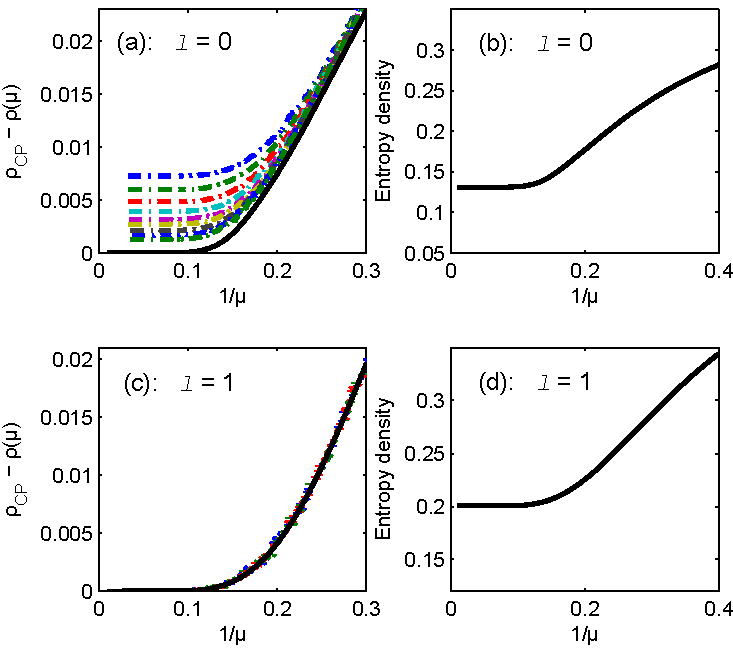
\includegraphics[width=1\columnwidth]{Chapter-2/Paper_HN5_PE_Plot}
\protect\caption{Reduced packing fraction and entropy density for HN5 from Wang-Landau
sampling and Simulated Annealing. (a)\&(b) are for $l=0$, and (c)
\&(d) are for $l=1$. The black solid lines represent the equilibrium
properties from Wang-Landau sampling with $N=1024$. The dotted lines
are from simulated annealing with $N=32,768$, run at different annealing
schedules with $d\mu=0.001/2^{j}$ for $j=0,\ldots,8$, from top to
bottom. As in Fig.~\ref{fig:HN3PE}, Wang-Landau sampling provides
the entropy density via Eq.~(\ref{eq:GCPdiff}), as shown in (b) and
(d).}
\label{fig:HN5PE} 
\end{figure}


\begin{figure}
\centering 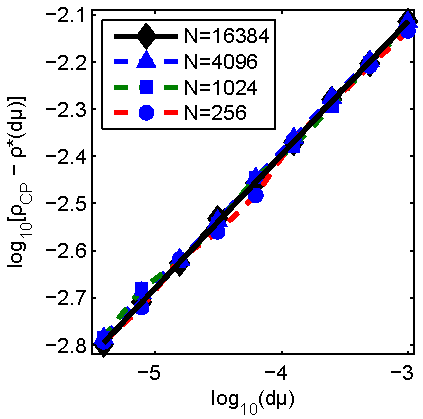
\includegraphics[width=0.5\columnwidth]{Chapter-2/Paper_HN5_Decay_Plot}
\protect\caption{Scaling of the dynamically reached packing fraction $\rho^{*}(d\mu)$
as a function of the annealing rate $d\mu$ for different system sizes
$N$ of HN5 for $l=0$, the dashed lines are for systems sizes $N=2^{k}$
with $k=8,10,12$, and 14. All data sets collapse onto the black solid line
with a slope of $0.31\pm0.01$ with $R^{2}=0.9989$, which is obtained
from a fit using the data of the largest system size $N=16,384$. Error
bars are about of the size of each data point or smaller, indicating
a relative error of less than $3\%$. }


\label{fig:HN5Decay} 
\end{figure}



\subsubsection{Results for HN5}

\label{subsec:HN5}

The case in HN5 is different from that in HN3. Note that HN5, unlike
HN3 and most finite-dimensional lattices or the random graphs studied
in Ref.~~\cite{Krzakala2008}, is not a regular network but has an exponential
degree distribution. In HN5 for both, $l=0$ and $l=1$, as shown
in Fig.~\ref{fig:HN5PE}, the equilibrium behavior obtained from Wang-Landau
sampling is smooth and there is no indication of a phase transition.
Annealing reveals a jamming transition and a power law decay similar
to that in HN3 in the dynamic simulations only for $l=0$. For $l=1$,
surprisingly, there is no jamming transition. The simulations with
different annealing schedules equilibrate easily and collapse with
the curves from Wang-Landau sampling. This suggests that the combination
of heterogeneity in neighborhood sizes together with the possibility
to have one occupied neighbor ``lubricates'' the system sufficiently
to avert jams. Correspondingly, the results from Wang-Landau converge
rapidly even for larger system sizes. As for HN3, permitting a local
hopping dynamics unjams the system also for HN5 with $l=0$.

\begin{figure}
\centering 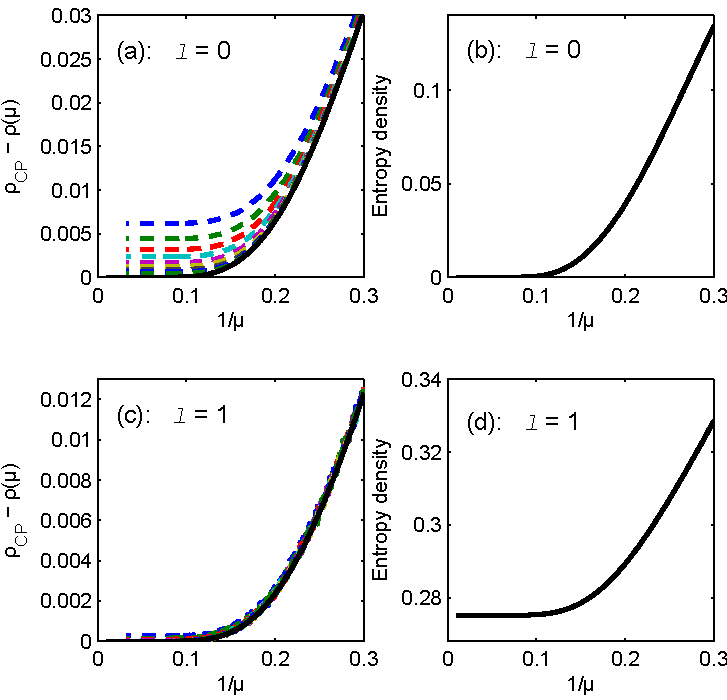
\includegraphics[width=0.95\columnwidth]{Chapter-2/Paper_HNNP_PE_Plot}
\protect\caption{Reduced packing fraction and entropy density for HNNP from Wang-Landau
sampling and Simulated Annealing. (a)\&(b) are for $l=0$, and (c)
\&(d) are for $l=1$. The black solid lines represent the equilibrium
properties from Wang-Landau sampling with $N=1024$. The dotted lines
are from simulated annealing with $N=16,384$, run at different annealing
schedules with $d\mu=0.001/2^{j}$ for $j=0,\ldots,8$, from top to
bottom. As in Figs. \ref{fig:HN3PE} and \ref{fig:HN5PE}, Wang-Landau
sampling provides the entropy density via Eq.~(\ref{eq:GCPdiff}),
as shown in (b) and (d). Note that in the limit of $\mu\to\infty$,
HNNP at $l=0$ has a zero entropy which corresponds to a unique ground
state. At $l=1$, it attains the \emph{same} close packing fraction,
$\rho_{CP}=\frac{1}{2}$, see Table \ref{tab:cpf}, but now at a non-trivial
entropy. }
\label{fig:HNNPPE} 
\end{figure}


\begin{figure}
\centering 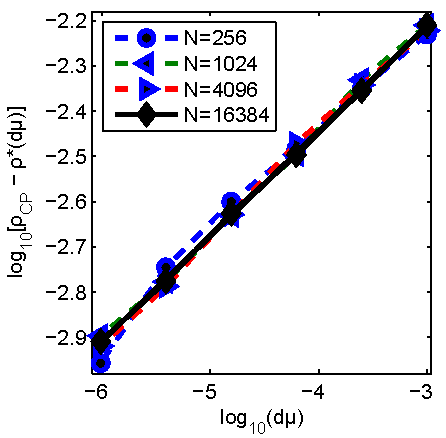
\includegraphics[width=0.5\columnwidth]{Chapter-2/Paper_HNNP_Decay}
\protect\caption{Scaling of the dynamically reached packing fraction $\rho^{*}(d\mu)$
as a function of the annealing rate $d\mu$ for different system sizes
$N$ of HNNP for $l=0$, the dashed lines are for systems sizes $N=2^{k}$
with $k=8,10,12$, and 14. All data sets collapse onto the top line
with a slope of $0.23\pm0.01$ with $R^{2}=0.9997$, which is obtained
from a fit using the data of the largest system size $N=16,384$. Error
bars are about of the size of each data point or smaller, indicating
a relative error of less than $3\%$. }

\label{fig:HNNPDecay} 
\end{figure}


\begin{table*}
\begin{centering}
\protect\caption{Summary of the results. \enquote{JT} means \enquote{ Jamming Transition }, and \enquote{PT} stands for \enquote{ Phase Transition }. For each network and the allowed neighborhood
occupations of $l=0$ and $l=1$, we list to potential for a jam in
dynamic simulations and the likely existence of an equilibrium glass
transition.}

\par\end{centering}

\begin{centering}
\label{tab:summary}
\par\end{centering}

\centering{}%
\begin{tabular}{|c|c||c|}
\hline 
 & $l=0$  & $l=1$ \tabularnewline
\hline 
\hline 
HN3  & JT \& no PT  & JT \& uncertain \tabularnewline
\hline 
HN5  & JT \& no PT  & No JT \& no PT \tabularnewline
\hline 
HNNP  & JT \& uncertain  & No JT \& no PT \tabularnewline
\hline 
\end{tabular}
\end{table*}



\subsubsection{Results for HNNP}

\label{subsec:HNNP}

HNNP provides an interesting alternative among the networks we are
considering here. Unlike HN3 and HN5, HNNP is a nonplanar network,
but like HN5 it has an exponential distribution of degrees with an
average degree of 4. Most importantly, HNNP at $l=0$ possesses a
``crystalline'' optimal packing that is unique, see Fig.~\ref{fig:HNNPPE}(b),
and consists of every second site along the line being occupied, i.e.,
those sites that uniformly have the lowest degree of 3. Therefore,
it provides the opportunity to explore the potential for a first-order
transition from a jammed state into the ground state, as was observed
for lattice glasses in Ref.~~\cite{Biroli02}. In this case, RG can
be applied to obtain $\rho(\mu)$ in equilibrium exactly.

Indeed, we find a weakly jammed state in HNNP with $l=0$, with only
a small number of frustrated particles, as shown in Fig.~\ref{fig:HNNPPE}.
The results of annealing simulations also show a power-law decay (Fig
\ref{fig:HNNPDecay}), consistent with the approach to a jamming transition.
As RG suggest, and the smooth equilibrium curve for $N=1024$ and
the convergence with increasing system sizes affirm, there is no thermodynamic
phase transition in HNNP with $l=0$. Despite the weakness of those
jams, we can find no indication that the annealing simulations at
any rate $d\mu$ can ever decay into the ordered state. Apparently,
the structural disorder, enforced in HNNP through a heterogeneous
neighborhood degree and the hierarchy of long-range links, prevents
such an explosive transition. The dominance of such structural elements
is further emphasized by the fact that HNNP for $l=1$ exhibits no
jams, similar to HN5, with which HNNP shares that structure. 


\section{Conclusions and Summary}

\label{sec:jam_conclusions}

We have examined the Biroli-Mezard lattice glass model on hierarchical
networks, which provide intermediaries between solvable mean-field
models and intractable finite-dimensional systems. These networks
exhibit a lattice-like structure with small loops but also with a hierarchy of long-range links
imposing geometric disorder and frustration while preserving a recursive
structure that can be explored with exact methods, in principle. We
observed a rich variety of dynamic behaviors in our simulations. For
instance, we find jamming behavior on a regular network for which
RG has shown that no equilibrium phase transition exists. However,
whether the dynamic transition occurs at a packing fraction distinctly
above random close packing remains unclear, and can only be resolved
with more detailed RG studies that are beyond our discussion here.

We have simulated the model on our networks with a varying chemical potential $\mu$,
with and without local hopping of particles. Hopping impacted those
simulations in a significant manner, always eliminating any jams that have existed without hopping. Solutions of the corresponding mean-field systems  would have suggested that a dynamics driven by hopping (but at fixed particle number) results in kinetic arrest~\cite{Rivoire03}. Whether canonical simulations with
hopping alone, or hopping at different rates, would change this scenario, we have to leave for future investigations, as well as the question
on whether a combined method of updates would alter the behavior observed
on lattices and mean-field networks.

\chapter{Antiferromagnetic Ising Model  in Hanoi Networks}
\label{chap-afm}
This chapter uses both computational and theoretical methods to study the dynamics and phase diagrams in antiferromagnetic Ising Model in Hanoi Networks.  First, the motivation of this study is reviewed in \ref{sec:amf-glass-intro}. Then two Monte Carlo methods are used to learn both the equlibrium and non-equlibrium properties for finite system sizes, which is described in \ref{sec:afm-mc}. In Sec. \ref{sec:afm-rg}, renormalization group is set up for both fixed point analysis and equlibrium properties explorations.  Using Monte Carlo methods and RG, spin glass phases, chaos, and a phase diagram are discovered in the model and networks, which is shown in Sec. \ref{sec:afm-results}.  

\section{Spin Glass Phase and Chaos in Antiferromagnets}
\label{sec:amf-glass-intro}
As introduced in Sec. \ref{sec:intro-afm}, the Ising antiferromagnet (AF) is a convenient model of glassy dynamics. With non-random interactions, it can still introduce geometric frustrations through complex structures and may give rise to a spin glass phase and glassy relaxation at low temperatures \cite{villain1977spin, herrero2008afm}. The motivations to this model in hierarchical networks are
\begin{itemize}
\item the antiferromagnetic Ising model (AFM) has been shown to have interesting dynamics \cite{shokef2011}, magnetization plateaus \cite{ohanyan2003mag} , and phase transitions\cite{herrero2008afm}, and even more interesting results are expected from our hierarchical networks;
\item the Hanoi networks are renormalizable and can be studied exactly \cite{boettcher2015classification, Boettcher2011HNNP}, which could provide more insights about the equilibrium dynamics underlying the extremely slow glassy dynamics;
\item the ferromagnetic Ising model in hierarchical networks has been studied  and shows phase transitions in Hanoi networks \cite{brunson2014rg}.
\end{itemize}

It is interesting to see how AFM behaves in these 4 hierarchical networks, HN3, HN5, HNNP, and HN6, whose short-range and long-range bonds create entangled loops of different sizes. These entangled loops can generate complex frustrations and introduce glassy dynamics and even phase transitions. 

First of all,  Wang-Landau algorithm is employed to investigate the energy landscape and the corresponding equilibrium behaviors for a range of different system sizes. Then simulated annealing is used to explore the dynamical behaviors, and an extremely slow relaxation is discovered at low temperatures, which also has a power-law scaling to different annealing schedules.  In addition to these two Monte Carlo methods, renormalization group is the main focus to study the equilibrium properties in the thermodynamic limit and to compare with the results from simulated annealing and Wang-Landau sampling. We discover three phases (ferromagnetic, paramagnetic, and spin glass phases) and an interesting phase diagram of the transitions. 


\section{Monte Carlo Methods}
\label{sec:afm-mc}
Similarly to the methods in Chater \ref{chap-jamming}, two Monte Carlo methods are used. Wang-Landau sampling is used to estimate the density of states, its energy landscape, and further equlibrium properties for finite system sizes; while simulated annealing can simulate experiments and the glassy dynamics.
 
\subsection{Wang-Landau Sampling}
Wang-Landau sampling is first introduced to estimate the density of states in ferromagnetic Ising model \cite{Wang2001}. Here we use it to calculate the density of states $g_{n}$ of AFM in
these 4 networks. Comparing to tradiation Ising model, AFM in Hanoi networks has entangled geometric frustractions, so we expect slower convergence and more computational complexity. From the experience in Jamming systems sampling, the sampling procedure for AFM in Hanoi networks is: 
\begin{enumerate}
\item Initially, set all unknown density of states $\{g_{E}=1\}$ and the
histogram $\{H_{E}=0\}$ for all energy states $E$, initiate the modification
factor $f=e^1$; 
\item Randomly pick a spin $i$ and flip it with a probability of $\min\left[1,\frac{g_{E_1}}{g_{E_2}}\right]$ where $E_1$ is the current state, and $E_2$ is the state if the spin is flipped;
\item Randomly pick 2 spins and exchange them to explore more states quickly; 
\item Update the $H_{E}$ and $g_{E}$ of the current state, i.e., set $\{H_{E}=H_{E}+1\}$
and $\{g_{E}=g_{E}\times f\}$; 
\item Repeat steps 2 to 4 until the sampling reaches a nearly flat histogram
for the $H_{E}$, then update the modification factor $f=\sqrt{f}$
and reset $\{H_{E}=0\}$; 
\item Stop if $f\le1+10^{-8}$. 
\end{enumerate}

The goal of Step 3 is to facilitate the random walk to explore phase space more broadly and to expedite convergence. We test the computations both with and without Step 3. However, no significant difference of computational efficiency is found, which is very different from the effect in Chapter \ref{chap-jamming}. The difference effect may be due to the intrinsically different interaction models. Exchanging in Jamming system only changes the configuration within the same occupation number $n$; while exchanging in AFM changes both the configuration and the energy, which is equivalent to randomly flipping of 2 sites.  

Due to geometric frustrations, Wang-Landau sampling can only find convergence for system size of up to $N\sim10^{3}$ within $\sim70$ hours of sequential computation. From the density of states, we can calculate the equilibrium thermodynamical properties for the corresponding system sizes, which is included in Sec. \ref{sec:afm-results}. 

\subsection{Simulated Annealing}
One of the most interesting phenomena in AFM is its glassy dynamics which can be learnt using Monte Carlo simulation. In this work, a canonical Monte Carlo method, Simulated Annealing ~\cite{SA}, is used to explore the dynamics from high to low temperatures. 

Similarly to the study of jamming in Chapter ~\ref{chap-jamming}, the Monte Carlo simulation can be considered as an experiment. The corresponding experiment is randomly flipping spins in the networks under a certain temperature $T$.  The standard procedure of the simulated annealing ~\cite{Vcerny1985} is adopted in this model. In the simulation, the procedure of the annealing algorithm is: 
\begin{enumerate}
\item Initially, start with a high temperature $T_{0}=10$ ; 
\item Randomly pick a spin on a lattice site $n$ to propose a flip; 
\item Flip the selected spin with a probability of $\min\left[1, \exp(-\Delta E /T)\right]$ 
where $\Delta E$ is the potential energy change if the spin is flipped; 
\item If exchange is allowed, randomly pick 2 neighbor-spins and exchange with a probability of $\min\left[1, \exp(-\Delta E /T)\right]$; 
\item Increase $T$ by $dT$ every 1 Monte Carlo sweep ($N$ random
updates), where $dT/dt$ (in time-units of $dt=1$ ) is the annealing
schedule and $dT\ll1$; 
\item Repeat steps 2 to 4 until $dT$ reaches a certain low temperature $T=1e-3$. 
\end{enumerate}

Step 4 is not a standard procedure in simulated annealing. The goal is to test the effect of local dynamics, similar to what is used in Chapter \ref{chap-jamming}. However, there is no significant difference in the results, while jamming states are eliminated in Chapter \ref{chap-jamming}. The reason of that may be similar to what we observe in Wang-Landau sampling, which is due to model differences.Detailed results are shown in Sec. \ref{sec:afm-results}.



\section{Renormalization Group}
\label{sec:afm-rg}
Renormalization Group (RG) is applied to these 4 Hanoi networks (HN3, HN5, HNNP, and HN6) which are suitable for decimation transformation in RG. The standard procedure developed for FM model by Boettcher, {\it et. al.} \cite{Boettcher2011HNNP, boettcher2015classification} is used in the AFM here, too. First, the general approach of RG on Hanoi networks is introduced; then the AFM Hamiltonians without and with external fields for these 4 networks is specifically set up and derived for RG.


\subsection{RG on Hanoi Networks}
\label{sec:afm-rghns}
The Hanoi networks are constructed hierarchically which is inherently suitable for RG. As in the stardard RG procedures, the spins in HNs are also hierarchically traced out level by level \cite{Boettcher2011HNNP, brunson2014rg}. For example, the site $n$ in HNs can be described by Eq. \ref{eq:numbering} ( $n(i,j)=2^{i-1}(2j+1)$ ), then the spins are traced out from level $i=1$ level by level. In the end, there is only 3 \enquote{spins} left, and all the Hamiltonian is renormalized to the bonds among these 3  \enquote{spins}.

\begin{figure}
\centering 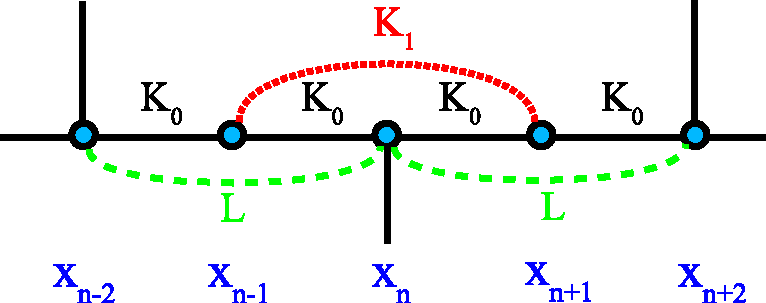
\includegraphics[scale=0.68]{Chapter-3/RG3hanoi}
\protect\caption{HN3 five-spin RG unit with all the couplings among the spins. $K_0$ and $K_1$ are actual bonds (connections) in HN3; while $L$ is emerged in the RG steps.}
\label{fig:afm-hn3rgbefore} 
\end{figure}

In terms of the 4 specific Hanoi network, we start with the most simple one HN3. As shown in Fig. \ref{fig:afm-hn3rgbefore} \cite{Boettcher2011HNNP}, all the couplings are included in a RG unit of 5 spins. The interaction constant on the backbone is $K_0$ ($=\beta J_0$); the coupling through the long-range bonds is $K_1$ ($=\beta J_1$); and $L$ is the emerging interaction which is initially 0.

\begin{figure}
\centering 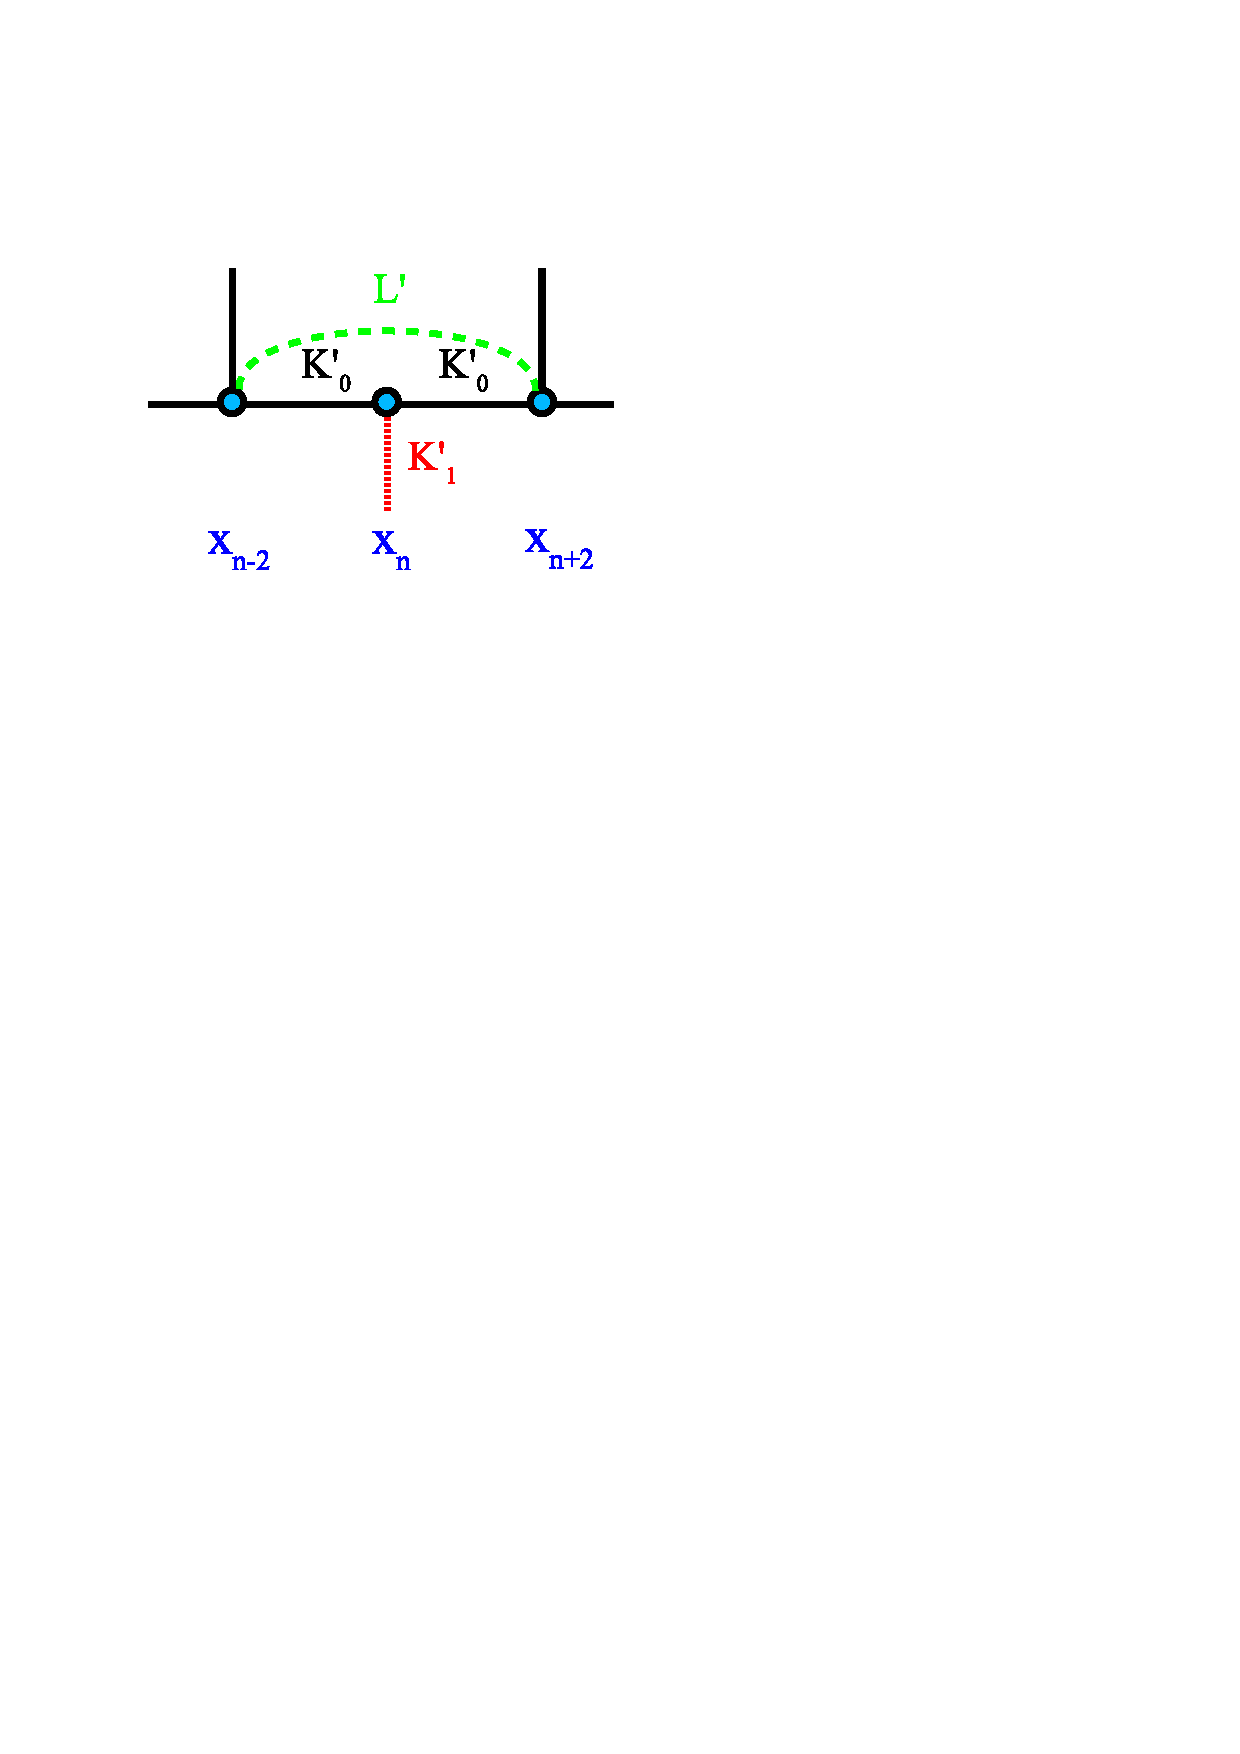
\includegraphics[scale=0.68]{Chapter-3/RG3hanoi_after}
\protect\caption{Hanoi networks three-spin graph after tracing over $x_{n\pm 1}$.}
\label{fig:afm-hn3rgafter} 
\end{figure}

After tracing over the odd spins $x_{n\pm 1}$, the long-range coupling as well the $K_0$ and $L$ between low-level sites is renormalized into $K_0 '$ and $L'$. The depiction of the graph left is shown in Fig. \ref{fig:afm-hn3rgafter} \cite{Boettcher2011HNNP}, which is about {\it half} of  Fig. \ref{fig:afm-hn3rgbefore} \cite{Boettcher2011HNNP}. $K_1 '$ in Fig. \ref{fig:afm-hn3rgafter} \cite{Boettcher2011HNNP} connects to another adjecent {\it half}, which produces another five-spin RG unit. By recursively renormaling the graph, the system size is reduced exponentially, and the final graph simply has 3 spins but very complicated couplings $K_0 ', K_1 ' $ and $L'$. The most important part in RG is to calculate these renormalized couplings.


\begin{figure}
\centering 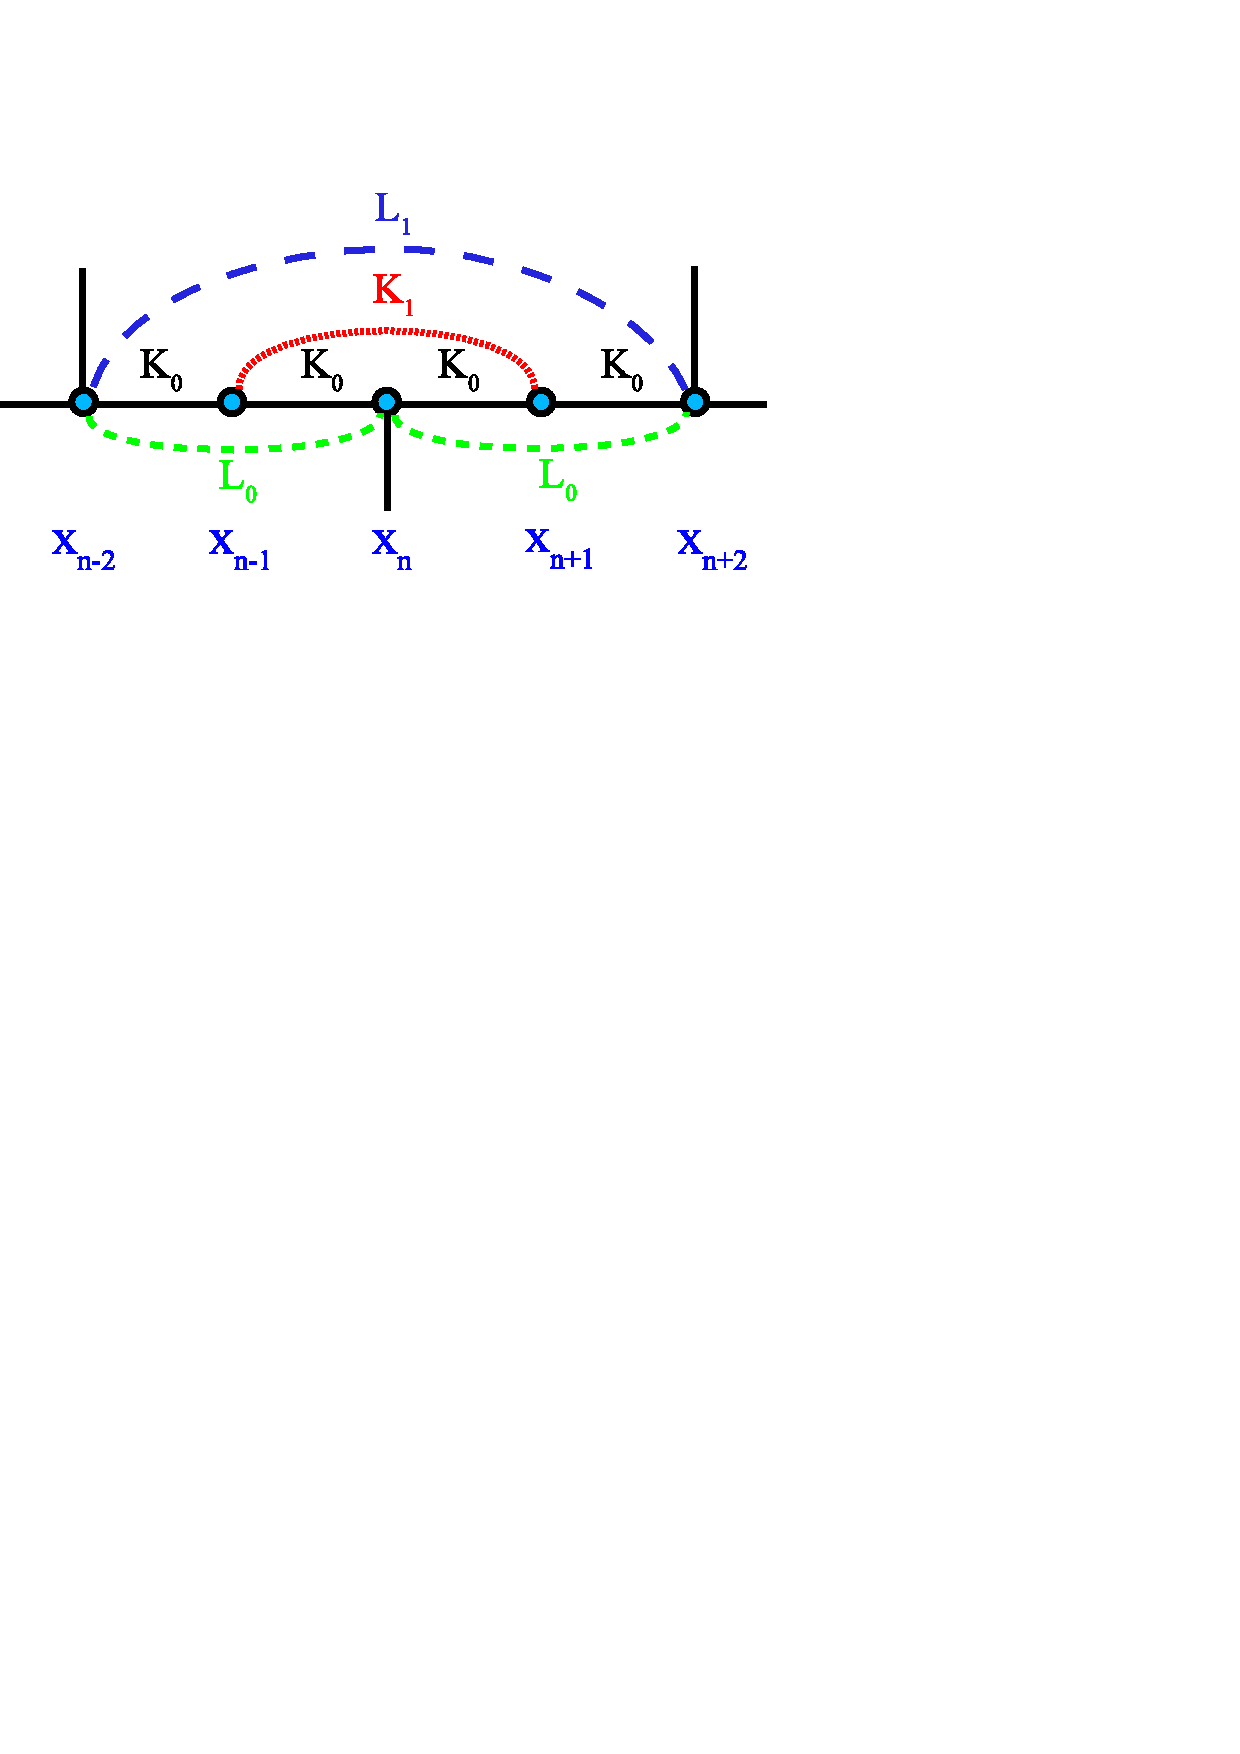
\includegraphics[scale=0.68]{Chapter-3/IsingRG_HN5_before}
\protect\caption{HN5 five-spin RG unit with all the couplings among the spins.}
\label{fig:afm-hn5rg} 
\end{figure}

\begin{figure}
\centering 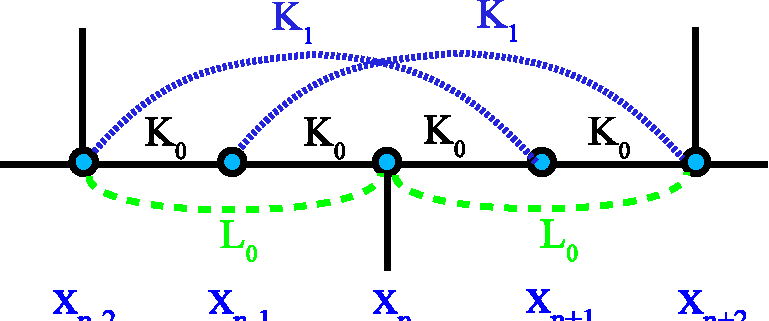
\includegraphics[scale=0.68]{Chapter-3/IsingRG_HNNP_before}
\protect\caption{HNNP five-spin RG unit with all the couplings among the spins.}
\label{fig:afm-hnnprg} 
\end{figure}

\begin{figure}
\centering 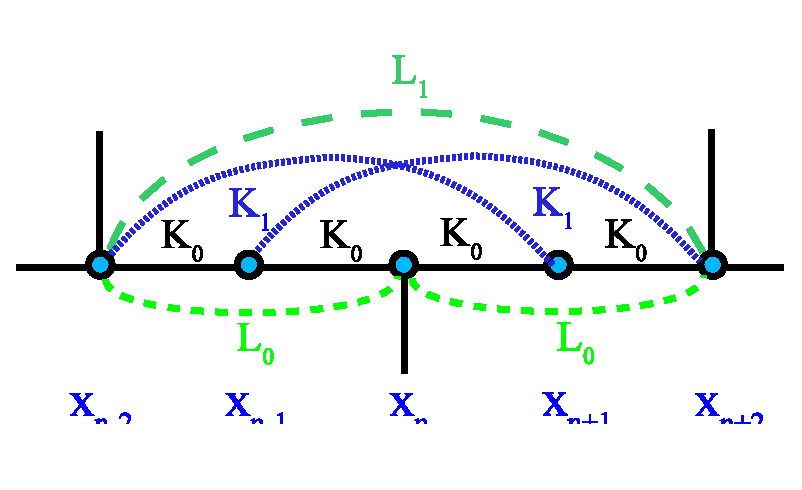
\includegraphics[scale=0.68]{Chapter-3/IsingRG_HN6_before}
\protect\caption{HN6 five-spin RG unit with all the couplings among the spins. $L_1$ is another interaction term emerging in the RG steps.}
\label{fig:afm-hn6rg}
\end{figure}

In addition to HN3, the other three networks have different setup of the five-spin RG unit but the same three-spin renormalized RG graph. The 5-spin graphlets are shown in Fig. \ref{fig:afm-hn5rg} \cite{Boettcher2011HNNP} for HN5, in Fig. \ref{fig:afm-hnnprg}  \cite{Boettcher2011HNNP} for HNNP, and in Fig. \ref{fig:afm-hn6rg} \cite{Boettcher2011HNNP} for HN6. 



\subsection{RG without magnetic fields}
The setup of RG is started by separating the AFM's Hamiltonian into hierarchies
\begin{equation}
-\beta\mathcal{H} = \sum_{n=1}^{k-2} (-\beta \mathcal{H}_n)+ \mathcal{R}(K_2, K_3, \cdots)
\end{equation}
where $\mathcal{R}$ is the coupling beyond $\mathcal{H}_n$ of levels $k>2$. $\mathcal{H}_n$ depends on the interactions $K_0$ on the backbone and $L_0$, $L_1$, $K_1, \cdots$ among the long range couplings. The detailed RG procedure is described network by network. 

\subsubsection{HN3, HN5, and their interpolations }
\label{sec:afm-HN35RG}

For HN3 and HN5, the Hamiltonian $\mathcal{H}_n$ for each hierarchy with 5 Ising spins is
\begin{eqnarray}
\label{eq:hn35-z0}
 -\beta \mathcal{H}_n &=& K_0 \left(x_{n-2}x_{n-1} + x_{n-1}x_{n} +  x_{n}x_{n+1} +  x_{n+1}x_{n+2}\right) \nonumber \\ 
   && + K_1(x_{n-1}x_{n+1}) + L_0(x_{n-2}x_{n} + x_{n}x_{n+2}) \nonumber \\
   && + y L_1 (x_{n-2} x_{n+2})  + 4I 
\end{eqnarray}
where $y$ is 0 for HN3 and 1 for HN5. $y$ can be extended to a wide range of parameters from $-\infty$ to $+\infty$, which leads to the interpolations of HN3 and HN5. These interpolations may introduce more interesting phases and transitions. $K_0$ is the interaction term of the 1D backbone. In terms of traditional Ising model's interaction term $J_0$, $K_0=\beta J_0$ which is usually $\beta=-1/T$ by setting $J_0=-1$ for AFM. The long range links over the same hierarchies have the coupling term $K_1$ ($=\beta J_0$) which is set as a constant in this RG flow. $L_0$ also stands for the coupling term emerged in the RG flow, and its initial value is 0. $L_1$ is accounted for the extra long range links in HN5 comparing to HN3. The last term $I$ is a constant emerging after the first step of RG, and its initial value is 0. Its coefficient $4$ is a simply a mathematical choice because there are effectively 4 spins in each hierarchy. The \underline{\emph{initial values}} for these parameters are
\begin{equation}
\begin{array}{l}
\displaystyle I = 0 \\
\displaystyle K_0 =\beta J_0=-\frac{1}{T} < 0 \\
\displaystyle K_1 =\beta J_0=-\frac{1}{T}  < 0 \\
\displaystyle L_0 = 0 \\
\displaystyle L_1 =\beta J_0 =-\frac{1}{T} < 0 \\
\end{array} 
\label{eq:hn35-init1}
\end{equation}
where Boltzmann constant $k$ is set as 1 here. $K_1$ is not changing in the RG flow because it is introduced again at every RG step. Therefore, it is equivalent to $-1/T$ which can be used as a reference to temperature. High temperatures $T \rightarrow \infty$ stands for $K_1\rightarrow -0$; while low temperatures $T\rightarrow 0$ corresponds to large $K_1 \rightarrow -\infty$.

After tracing over the sites $x_{n-1}$ and $x_{n+1}$, we can get this form of equation
\begin{equation}
\label{eq:hn35-z1}
 -\beta \mathcal{H}_n = 2I' +  K'_0 \left(x_{n-2}x_{n} +  x_{n}x_{n+2}\right) + L'_0(x_{n-2}x_{n+2})
 \end{equation}
 which is `half' of original RG setup.
For the convenience of mathematical and computational analysis, these parameters is transformed to a new set of activity parameters  
\begin{equation}
\begin{array}{l}
\displaystyle C = e^{-4I}   \\
\displaystyle \kappa = e^{-4K_0} \\
\displaystyle \lambda = e^{-4L_0}  \\
\displaystyle \mu = e^{-2K_1} = e^{-2L_1} 
\end{array} 
\label{eq:hn35-activities}
\end{equation}
The pre-factors of $K_0, K_1, I ,$ and $ L_1$ is for the convenience of the RG calculations. Thus, the  new \underline{\emph{initial values}}  are


\begin{equation}
C = 1,   \kappa = \mu^2 > 1, \lambda =\mu^{2y} , \mu >1 
\label{eq:hn35-init1}
\end{equation}
where $\mu$ is equal to $e^{2/T}$ since $K_1$ is set as a constant of $-1/T$. Apparently, only $\mu$ needs to be specified to start the numerical RG flow. In other words, the initial values for HN3($y=0$) and HN5($y=1$) are determined by $\mu$ and $y$.

To establish an intuitive connection to these defined RG parameters, the relationship between $\mu$ and $T$ is ,  
\begin{equation}
\begin{array}{l}
\displaystyle T\rightarrow 0 \ \Leftrightarrow \ \ K_1 \rightarrow -\infty  \ \Leftrightarrow \ \ \mu \rightarrow \infty   \ \Leftrightarrow  \ \ {1}/{\mu}\rightarrow 0+\\
\displaystyle T\rightarrow \infty  \ \Leftrightarrow  \ K_1 \rightarrow 0- \ \Leftrightarrow  \ \ \mu \rightarrow 1+ \  \ \Leftrightarrow  \ \  {1}/{\mu}\rightarrow 1- \\
\end{array} 
\label{eq:Ts}
\end{equation}
, and the relationship among $\kappa$, $J_0$, temperature $T$, and $\mu$ is
\begin{equation}
\begin{array}{l}
J^{(0)} = -1,  \\ 
T = 2/\log(\mu) \\ 
J^{(n)} = -\frac{T}{4}\log\kappa^{(n)} \\
\end{array}
\label{eq:afm-hn35-jk}
\end{equation} 
where $J^{(0)}$ stands for the initial value in the RG flow and is the same as $J_0$, and $J^{(n)}$ and $\kappa ^{(n)}$ are the $i$-th renormalized variables.

By tracing over all the $\{x_n\}$ in Eq. \ref{eq:hn35-z0} and Eq. \ref{eq:hn35-z1}, we can get $2^{3}$ equations with 3 unknown variables ($ K_0,  L_0, I$). The solutions in terms of $(\kappa, \lambda, C)$ are
\begin{equation}
\begin{array}{l}
\displaystyle \kappa' = \frac{2\kappa \lambda (1+\mu) }{\kappa^2+2\mu \kappa +1} \\
\\
\displaystyle \lambda' = \mu^{2y} \frac{(1+\mu)(1+\kappa)^2}{2(\kappa^2+2\mu \kappa +1)}\\ \\
\displaystyle C' =  \frac{C^2 \kappa\mu}{\sqrt{2} (1+\kappa) (1+\mu)^{3/2}  \sqrt{ \kappa^2+2\mu \kappa +1}}   \\
\end{array} 
\label{eq:afm-hn35sol1}
\end{equation}

These solutions are the same as the RG process in FM Ising model \cite{Boettcher2011HNNP}, but the RG results afterward are very different due to the inherent frustrations and complexity in AFM. The fixed point analysis is continued in Sec. \ref{sec:afm-results}.



\subsubsection{ HNNP, HN6, and their interpolations }
The initial RG setup of planar networks, HN3 and HN5, has been described in the previous subsection. While the non-planar networks, HNNP and HN6, share a similar setup except for different interaction terms due to different long-range links in these small-world networks. The $\mathcal{H}_n$ for each hierarchy is 
\begin{eqnarray}
 -\beta \mathcal{H}_n &=& K_0 \left(x_{n-2}x_{n-1} + x_{n-1}x_{n} +  x_{n}x_{n+1} +  x_{n+1}x_{n+2}\right) \nonumber \\ 
   && + K_1(x_{n-2}x_{n+1} + x_{n-1}x_{n+2}) + yL_1(x_{n-2} x_{n+2}) \nonumber \\
   && +L_0(x_{n-2}x_{n} + x_{n}x_{n+2})  + 4I 
\label{eq:hp-z0}
\end{eqnarray}
where $y$ is 0 for HNNP and 1 for HN6. The interpolations of HNNP and HN6 can also be easily explored using different $y$'s. $K_0$ ($=\beta J_0= -1/T$) is the interaction term of the 1D backbone. $K_1$ ($=\beta J_0$) is also set as a constant $\beta J_0$ ($=-1/T$). $L_0$ is an emerging terms after the first RG step, and $L_1$ is for the extra long range links in HN6 comparing to HNNP. $I$ is still a constant. The \underline{\emph{initial values}} for these parameters are All the initials values for these activity parameters are
\begin{equation}
\begin{array}{l}
\displaystyle I = 0 \\
\displaystyle K_0 =\beta J_0=-\frac{1}{T} < 0 \\
\displaystyle K_1 =\beta J_0=-\frac{1}{T}  < 0 \\
\displaystyle L_0 = 0 \\
\displaystyle L_1 =\beta J_0 =-\frac{1}{T} < 0 \\
\end{array} 
\label{eq:hp-init1}
\end{equation}

By tracing the sites $x_{n-1}$ and $x_{n+1}$, the reduced form of Hamiltonian with 3 spins is
\begin{equation}
\label{eq:hnnpz1}
 -\beta \mathcal{H}_n = 2I' +  K'_0 \left(x_{n-2}x_{n} +  x_{n}x_{n+2}\right) + L'_0(x_{n-2}x_{n+2})
 \end{equation}
 which is the same as that in HN3 and HN5. Similarly, a new set of parameters is introduced, and their definitions and possible values are  
 \begin{equation}
\begin{array}{l}
\displaystyle C = e^{-4I} > 0   \\
\displaystyle \mu = e^{-2K_1} = e^{-2L_1} > 1 \\
\displaystyle \kappa = e^{-4K_0} > 1 \\
\displaystyle \lambda = e^{-4L_0}  > 1\\
\end{array} 
\label{eq:hn35-activities}
\end{equation}
Their corresponding initial values are 
 \begin{equation}
 C = 1,  \kappa = \mu^2,  \lambda =  \mu^{2y} 
\label{eq:hp-init2}
\end{equation}
where $y$ can be 0 for HNNP, 1 for HN6, and any other values for thier interpolations. All the initials values for these activity parameters are the same as in HNNP. The RG recursive equations are
\begin{equation}
\begin{array}{l}
\displaystyle \kappa' = \frac{\kappa \lambda (1+\mu)^2 }{(1+\mu\kappa)^2} \\
\\
\displaystyle \lambda' =\mu^{2y} \frac{(\kappa + \mu)^2} {(1 + \mu \kappa)^2} \\ \\
\displaystyle C' =  \frac{C^2 \kappa\mu^2} {(1+\mu)^2 (\kappa+\mu) (1+ \mu\kappa)}   \\
\end{array} 
\label{eq:afm-hpsol1}
\end{equation}
These solutions are also the same as those in Ref. \cite{Boettcher2011HNNP}, but we expect possible glassy and chaotic behaviors introduced in AFM and these complex networks.


\subsection{RG with magnetic fileds}
In order to study a broad range of physical properties using RG, the external magnetic field $H$ is needed. We plan to explore different physical properties, such as internal energy $e$, magnetization $m$, free energy $f$, entropy $s$, specific heat $c_v$, and magnetic susceptibility $\chi$. 

Here the RG setup is extended to a more general scenario by including $H$. The procedure of such RG has been developed by Brunson and Boettcher in FM of Hanoi networks \cite{brunson2014rg}. In AFM, the same procedure is followed with corresponding adjustments of temperature $T$ ($\mu$ in RG) and prefactors of these derivations. Instead of detailed derivations \cite{brunson2014rg}, only the general logic and the formulations of targeted physics properties are described in this section. 

The starting point of all these equilibrium physical properties is the partition function $Z$. As shown in Fig. \ref{fig:afm-hn3rgafter}, the partition function of the smallest system size $N=2^1+1=3$
\begin{equation}
Z^{(1)} = e^{-\beta \mathcal{H} ( K^{(1)}, L^{(1)}, \cdots ;\  x_1, x_2, x_3)}
\end{equation}
where $K^{(1)}, L^{(1)}, \cdots$ stands for the raw activity parameters of temperature $T$, coupling $J$, and magnetic field $H$; $x_1, x_2$, and $ x_3$ are the 3 spins ($\pm 1$). 
Using RG and its recursive solutions (similar to Eq. \ref{eq:afm-hn35sol1} in RG without magnetic field), it is easy to obtain the renormalized activity parameters  $K^{(n)}, L^{(n)}, \cdots$. The superscript $n$ means system size $N=2^n + 1$. 

The physical properties calculated are
\begin{enumerate}
\item internal energy per spin
\begin{equation}
e = -\frac{1}{N}\frac{\partial \ln Z}{\partial \beta}
\end{equation}
The goal is to find the equilibrium energy to uncover the non-equilibrium dynamics in simulations.

\item Free energy per spin
\begin{equation}
f = - \frac{1}{N}\frac{1}{\beta} \ln Z
\label{eq:afm-free}
\end{equation}

\item Free energy difference between parallel and anti-parallel boundary conditions

The equation of the free energies is still the same as Eq. \ref{eq:afm-free}. The difference is that the first spin ($x_0$) and last one ($x_{N}$) are fixed, i.e., the parallel boundary condition ($f_1$) have both $x_0 = x_N = +1$, while the anti-parallel boundary condition ($f_2$) has $x_0=+1$ but $x_N=-1$. The difference is
\begin{equation}
\Delta f = f_1 - f_2 = - \frac{1}{N}\frac{1}{\beta} ( \ln Z_{++} - \ln Z_{+-}) =- \frac{1}{N}\frac{1}{\beta}  \ln \frac{Z_{++}}{ Z_{+-}}
\label{eq:afm-freediff}
\end{equation}
where $Z_{++}$ and $Z_{+-}$ stand for the partition functions of parallel and anti-parallel boundary conditions, respectively.

The goal of this parameter is to discover the chaotic dynamics and spin glass phase. In a spin glass system with chaotic dynamics, the difference $\Delta F$ is non-zero in the thermodynamic limit and changes signs at different temperatures \cite{wang2015chaos}. In a range of temperatures, the number of times of changing sign of $\Delta F$ may increase  with system size following a power-law. 

\item entropy per spin
\begin{equation}
s = \frac{1}{N} \frac{\partial}{\partial T} \left( \frac{1}{\beta} \ln Z \right)
\end{equation}
Entropy may be useful to understand the geometric frustrations and compared to Wang-Landu sampling's density of states. 

\item magnetization per spin
\begin{equation}
m = \frac{1}{N}\frac{1}{\beta} \frac{\partial \ln Z}{\partial H}
\end{equation}
The magnetization may have interesting patterns at low temperatures \cite{ohanyan2003mag, kageyama2000direct} due to complex local spin configurations.

\item specific heat per spin
\begin{equation}
c_v = \frac{\partial e} {\partial T}
\end{equation}
If there is any second-order phase transition, specific heat $c_v$ may show the transition.

\item magnetic susceptibility per spin
\begin{equation}
\chi = \frac{\partial m} {\partial H}
\end{equation}
If there is any second-order phase transition, susceptibility  $c_v$ may show the transition.

\end{enumerate}

There equations are trivial and can be found in the textbook, but their implementation in RG take a large amount of analytical deviations and numerical testing. The detailed description can be found in the work by Brunson and Boettcher \cite{brunson2014rg}.


\section{Results}
\label{sec:afm-results}
The most common observations in AFM with geometric frustraions are the glassy dynamics at low temperatures, which is often observed in experiments and simulations. However, the equlibrium behaviors near and beyond the critical point can only be detected using analytical method. Using both the computational and analytical methods introduced the previous section, results of dynamic properties, fixed point analysis, and corresponding equlibrium properties are described in Sec. \ref{sec:afm-dyn}, Sec. \ref{sec:afm-fpa}, and Sec. \ref{sec:afm-eqa}, respectively.

\subsection{Dynamic Properties}
\label{sec:afm-dyn}
The interesting glassy dynamics can be observed from simulational experiments using simulated annealing described in Sec. \ref{sec:afm-mc}. In the simulations, the only control parameter is the temperature $T$. The starting point is high $T$ ($T=10.0$) which corresponds to 
 paramagnetic disordered states. As the $T$ is decreased, the system is more and more likely to
 accept a transition to a lower energy state. In a system with no geometric frustrations, a low $T\rightarrow0$ would lead to the ground state with the lowest energy. However, AFM in Hanoi networks cannot reach ground states due to complex geometric frustrations. 

\begin{figure}
\centering 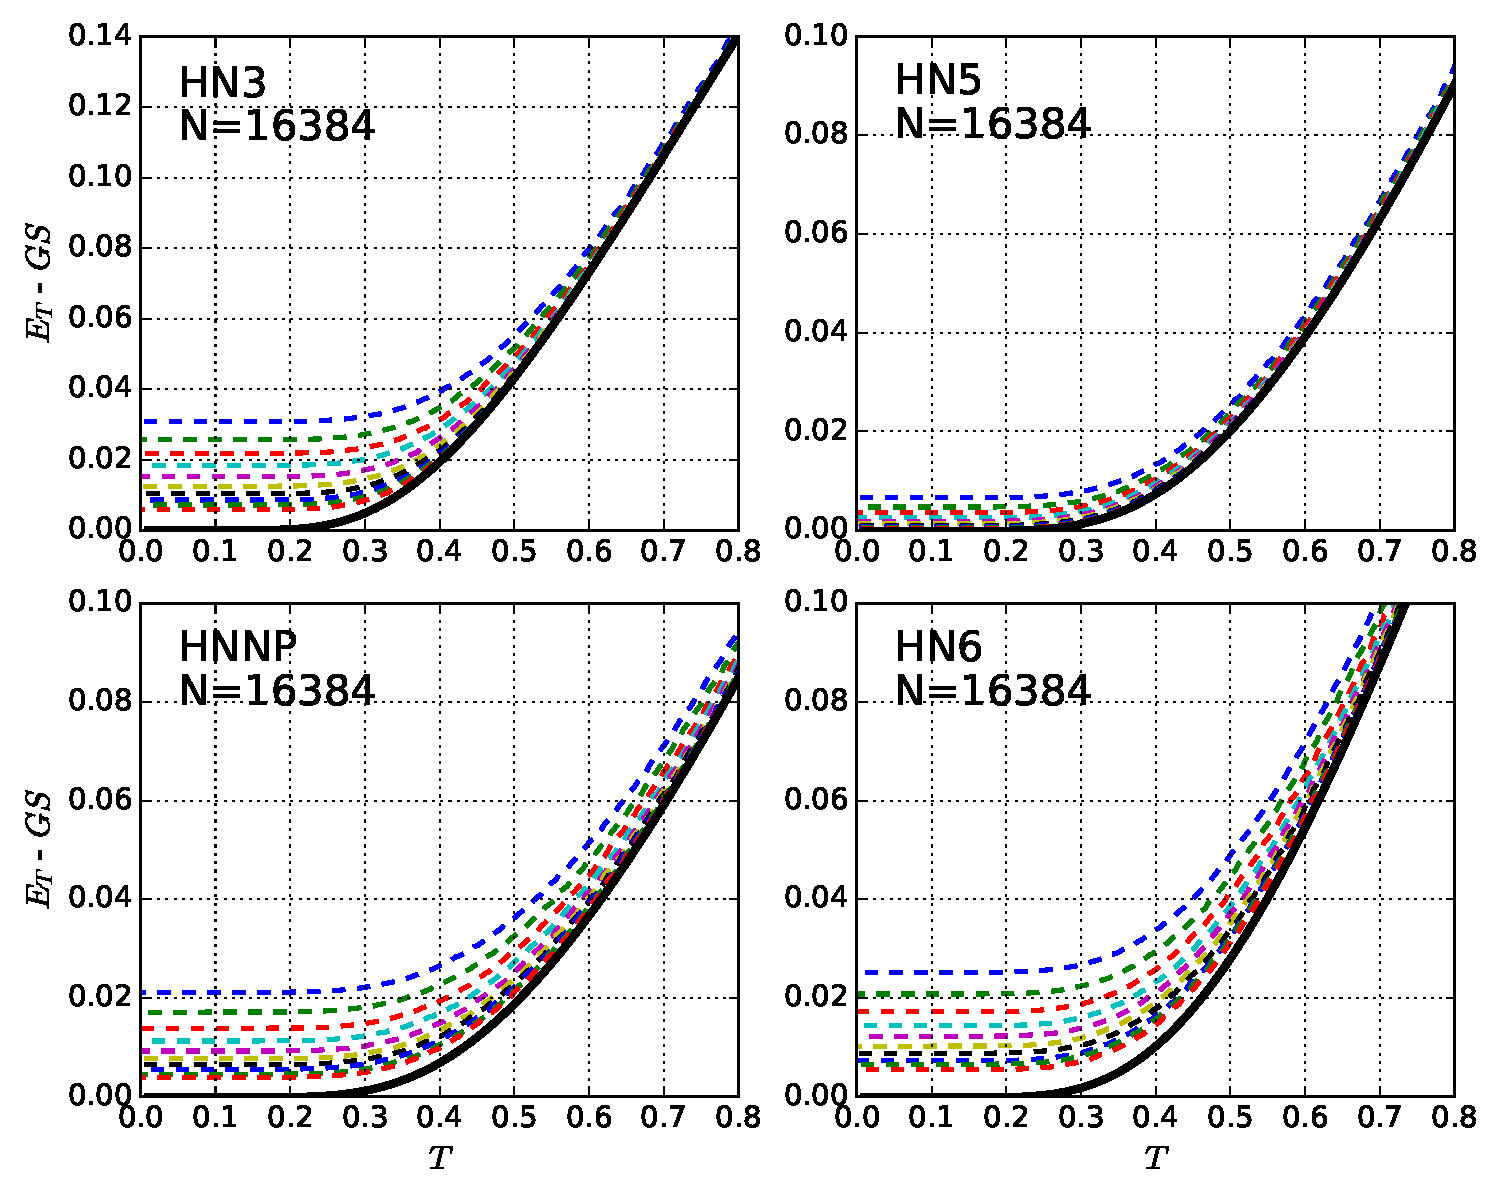
\includegraphics[width=0.9\columnwidth]{Chapter-3/AFM_Jamming_SA_plot}
\protect\caption{Energy vs. temperature $T$ from the Simulated Annealing of all the four networks. In each of the 4 subfigures, the dotted curves from top to bottom correspond to annealing schedules of $10^{-3},  10^{-3}/2^1, 10^{-3}/2^2, \cdots, 10^{-3}/2^9$, respectively. The slowest annealing schedule is $1.95\times10^{-6}$. The solid black curves on the bottom are the equilibrium curves from RG, which clearly shows the gap between equilibrium and non-equilibrium behaviors.}
\label{fig:afm-hnsjam} 
\end{figure}

The behavior at low $T$ is similar to what is observed in the jamming systems in Chapter \ref{chap-jamming}. As shown in Fig. \ref{fig:afm-hnsjam} and \ref{fig:afm-hnsscaling}, all four
 networks show the glassy dynamics with a power relaxation. HN5 may reach equilibrium ground
 states at a much slower annealing schedules due to increasing variations at lower schedules. Other networks have clearly a gap between 'jammed' state and the equilibrium ground states, and the gap can only be eliminated at an infinitely slow annealing rate after an infinitely long time due to the power-law scaling.

\begin{figure}
\centering 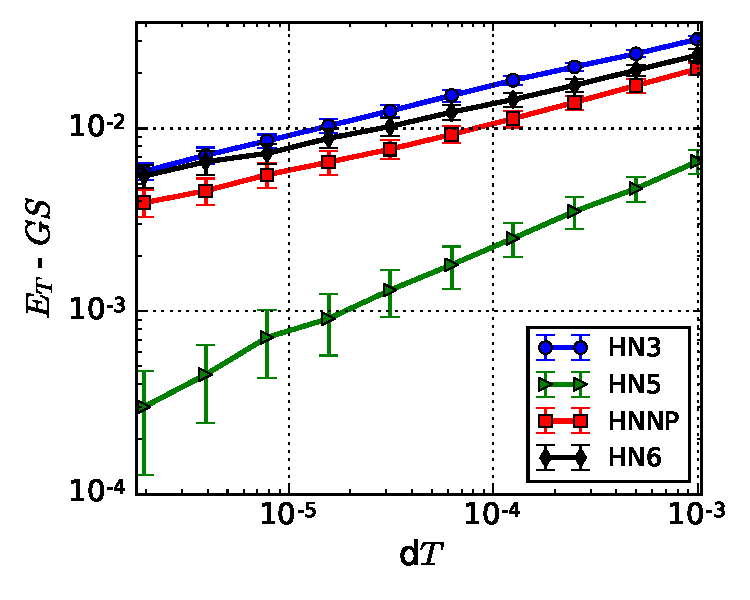
\includegraphics[width=0.5\columnwidth]{Chapter-3/AFM_Jamming_SA_scaling_plot}
\protect\caption{Scaling of  dynamically reached lowest energy at different annealing schedules. The error bar is calculated from $100$ or more runs with different random initializations. The ground states are obtained using renormalization group.}
\label{fig:afm-hnsscaling} 
\end{figure}

In order to get the relaxation scaling in Fig. \ref{fig:afm-hnsscaling}, the most challenging part is to find the ground states. Unlike the exact and fractal "ground states" in the jamming systems, AFM in these four HNs has different but converging ground states as the system size gets larger and larger. Wang-Landu sampling fails to produce ground states for system sizes $N>2^{10}$, and renormalization group (RG) has to be used to find the ground states at different system sizes. From RG calculations, the equilibrium ground states for HN3, HN5, HNNP, and HN5 at system size $N=2^{14}$ are $-1.0$, $-1.166503...$, $-1.480224...$, $-1.285644...$, respectively.  More details of  RG and equilibrium properties are discussed in Sec. \ref{sec:afm-eqa}.

\subsection{Fixed Point Analysis}
\label{sec:afm-fpa}
Starting from the recursive solutions of Eq. \ref{eq:afm-hn35sol1} and Eq. \ref{eq:afm-hpsol1} in Sec. \ref{sec:afm-rg}, the fixed point analysis can help discover possible chaotic and critical behaviors. 

\subsubsection{ HN3, HN5, and their interpolations }
For HN3 with $y=0$ in Eq. \ref{eq:afm-hn35sol1}, there are 2 analytical fixed points which are
\begin{equation}
\displaystyle \kappa^* = 1, \lambda^* =1; 
\label{eq:afm-fps3-1}
\end{equation}
\begin{equation}
\displaystyle \kappa^* = 0, \lambda^* =\frac{1+\mu}{2} 
\label{eq:afm-fps3-2}
\end{equation}
where only the first one is a stable fixed point solution. The second one is only stable at the high temperature limit, and any finite temperatures lead to the fixed point $\kappa^* =1, \lambda^* = 1.$ The stability of the two fixed points is mathemtically analyzed using the Jacobian matrix later in this section.

HN5 with $y=1$ has more interesting fixed points are more interesting. The two fixed point solution are
\begin{equation}
\kappa^* = 0, \ \  \lambda^* = \mu^{2y}\frac{\mu+1}{2}
\label{eq:afm-fps5-1}
\end{equation}

\begin{equation}
\begin{array}{l}
\displaystyle \kappa^* = \frac{1}{2}\left[\mu^2 -\mu + \sqrt{(\mu+1)(\mu^3 - 3\mu^2 +8\mu-4)} \right]  \\  \\
\displaystyle \lambda^* = \frac{\mu}{4}\left[\mu^2 -\mu+2 + \sqrt{(\mu+1)(\mu^3 - 3\mu^2 +8\mu-4)} \right]
\end{array} 
\label{eq:afm-fps5-2}
\end{equation}

With different $y$,  the parameter of interest $\kappa$ in Eq. \ref{eq:afm-fps5-2} can be written in a general form as a function of $\mu$ ($\mu>1$) and $y$
\begin{equation}
\kappa^* = \frac{1}{2}\Big[\sqrt{4\left( \mu^{1+y} + \mu^{y} - 1\right)+\left( \mu^{1+y} + \mu^{y} - 2\mu\right)^2}+ 
\mu^{1+y}+\mu^{y} -2\mu \Big] 
\label{eq:afm-fyps_k}
\end{equation}
, and the corresponding $\lambda$ is
\begin{equation}
\lambda^* = \frac{\mu ^y}{4}  \left(2 \mu +\mu ^{y+1}+\mu ^y-\sqrt{(\mu +1) \left(4 \mu +\mu ^{2 y}+4 \mu ^{y+1}+\mu ^{2 y+1}-4 \mu ^y-4\right)}-2\right)
\label{eq:afm-fyps_l}
\end{equation}

The stability of the fixed points can be proved by both numerical iterations (as shown in Fig. \ref{fig:afm-HN35KJ_ys}) and the eigenvalue of the Jacobian from Eq. \ref{eq:afm-hn35sol1}. The Jacobian matrix is
\begin{equation}
  Jacobian(\kappa,\lambda; \mu) =
\left(\frac{\partial(\kappa', \lambda')}{\partial(\kappa, \lambda)}\right)=
\left( {\begin{array}{*{50}c}
J_{11} & J_{12}\\
J_{21} & J_{22}
 \end{array} } \right)
=
\left( {\begin{array}{*{50}c}
\frac{\partial \kappa'}{\partial \kappa}&\frac{\partial \kappa'}{\partial \lambda}\\
\frac{\partial \lambda'}{\partial \kappa}&\frac{\partial \lambda'}{\partial \lambda}\\
 \end{array} } \right)
\label{eq:hn35-j}
\end{equation}
where $Jacobian$ is used to avoid conflicts with the interaction constant $J$, and the matrix elements are
\begin{equation}
J_{11} = \frac{\partial \kappa'(\kappa, \lambda)}{\partial \kappa}=-\frac{2 (\kappa -1) (\kappa +1) \lambda  (\mu +1)}{\left(\kappa ^2+2 \kappa  \mu +1\right)^2}
\end{equation}
\begin{equation}
J_{12} =  \frac{\partial \kappa'(\kappa, \lambda)}{\partial \lambda}= \frac{2 \kappa  (\mu +1)}{\kappa ^2+2 \kappa  \mu +1}
\end{equation}
\begin{equation}
J_{21} =\frac{\partial \lambda'(\kappa)}{\partial \kappa}=\frac{(\kappa -1) (\kappa +1) (\mu -1) (\mu +1) \mu ^{2 y}}{\left(\kappa ^2+2 \kappa  \mu +1\right)^2}
\end{equation}
\begin{equation}
J_{22} = \frac{\partial \lambda'(\kappa)}{\partial \lambda}=0
\end{equation}

From the Jacobian matrix, it is easy to calculate the eigenvalues which is not shown here due to its complex and long form. The fixed points of Eq. \ref{eq:afm-fyps_k} and Eq. \ref{eq:afm-fyps_l} produce eigenvalue with magnitude less than 1, which means stable fixed points.

\begin{figure}
\centering 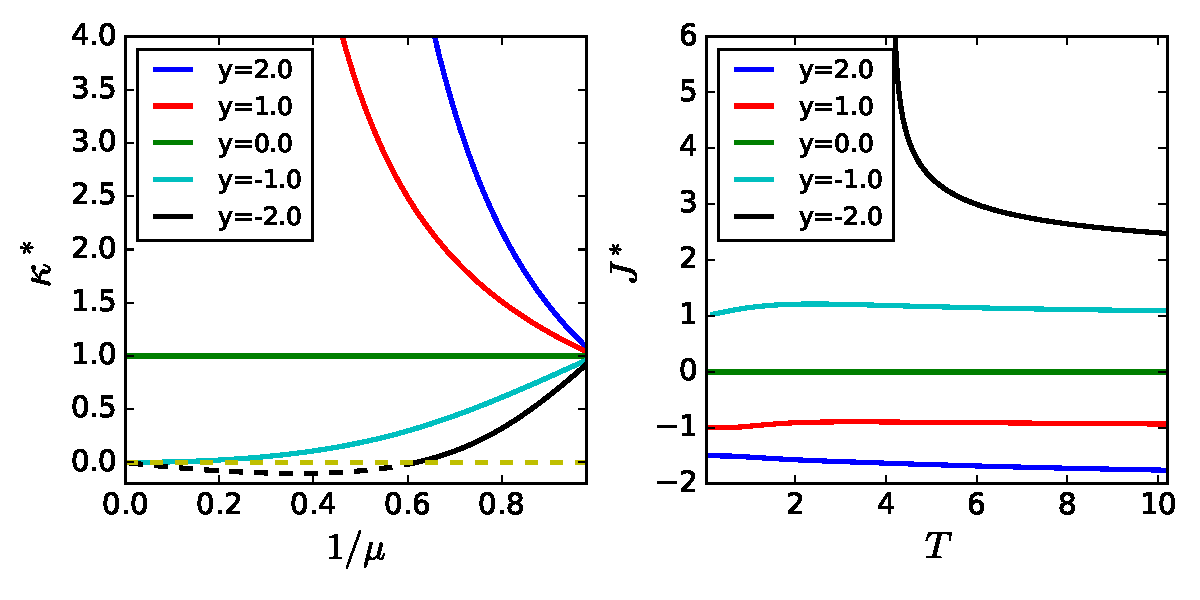
\includegraphics[width=0.9\columnwidth]{Chapter-3/HN35_KJvsTys.pdf}
\protect\caption{The numerical fixed points of $\kappa^*$ and corresponding $J^*$ using Eq. \ref{eq:afm-hn35-jk2} for HN3, HN5, and their interpolations. $y=0$ corresponds to HN3; $y=1$ corresponds to HN5; and $y<0$ corresponds that the extra bonds of HN5 comparing to HN3 are ferromagnetic. }
\label{fig:afm-HN35KJ_ys} 
\end{figure}


The fixed point as a function of temperature ($\mu$ or $T$) at different $y$'s are shown in Fig. \ref{fig:afm-HN35KJ_ys}. Equivalently, the fixed point of $\kappa^*$ is the converged renormalized $\kappa^*$ , and the corresponding interaction constant $J^*$ is the renormalized interaction constant in the thermodynamic limit. Based on Eq. \ref{eq:afm-hn35-jk}, the relationship between $\kappa^*$ and $J^*$ is
\begin{equation}
J^* = -\frac{T}{4} \log \kappa^*
\label{eq:afm-hn35-jk2}
\end{equation}




\begin{figure}
\centering 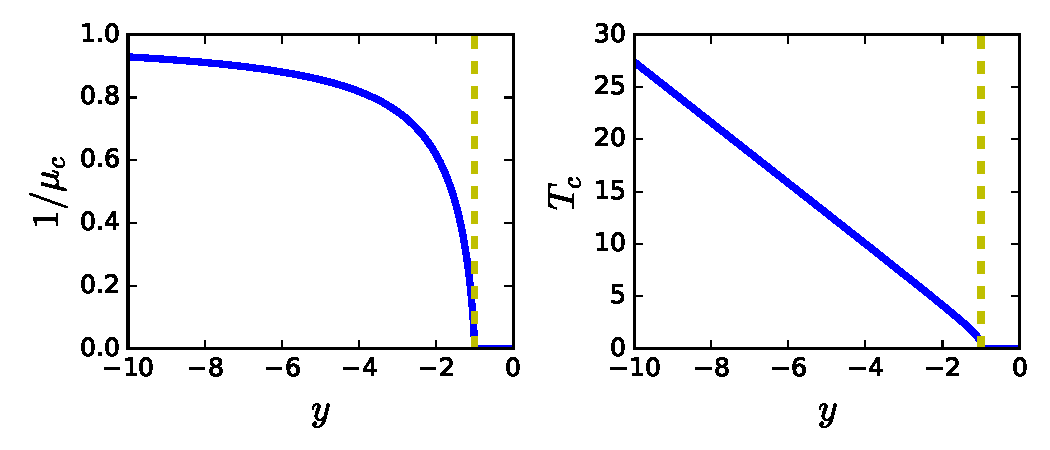
\includegraphics[width=0.9\columnwidth]{Chapter-3/HN35ysTransVsY.pdf}
\protect\caption{Transition temperatures at different $y$'s. This is also a phase diagram. The phase above the curves is the paramagnetic phase while the phase below the curve is the ferromagnetic phase. }
\label{fig:afm-hn35transys} 
\end{figure}

As shown in Fig. \ref{fig:afm-HN35KJ_ys}, $\kappa^*$ changes with temperature $\mu$. Similarly to FM Ising model \cite{Boettcher2011HNNP}, the values of $\mu$ satisfying $\kappa(\mu)=0$ are the phase transition temperatures. After transformation of Eq. \ref{eq:afm-fyps_k}, the equation $\kappa(\mu)=0$ can be rewritten as 
\begin{equation}
\mu^{1+y} + \mu^y -1 =0
\end{equation}
where there is a real root for $y\le-1.0$ in the antiferromagnetic range of $\mu>1$.  The transition temperature ($\mu_C$ or $T_C$) as a function of $y$ is shown in Fig.  \ref{fig:afm-hn35transys}.


\subsubsection{ HNNP, HN6, and their interpolations }

In the AFM scenario, for HNNP ($y = 0$), there are only 2 possible fixed points 
\begin{equation}
\kappa^* = 0, \ \lambda^* = \mu^2 
\end{equation} 
\begin{equation}
\kappa^* = \lambda^* = 1 
\end{equation} 
 The stability of HNNP is not uniform across different temperatures. The fixed point of $\kappa$ and $\lambda$ is 1 for $\mu \le 3$ ($T\ge1.820478\cdots$) and oscillating fixed points for $\mu > 3$ ($T<1.820478\cdots$). This result is obtained from both numerical iterations of $\kappa^*(\kappa, \lambda)$ and fixed point stability analysis from the Jacobian.
The simple numerical iterations of Eq. \ref{eq:afm-hpsol1} is shown in Fig. \ref{fig:afm-hnnpkappa}, and the absolute eigenvalue of Jacobian matrix is shown in Fig. \ref{fig:afm-hnnp_eigs}.
\begin{figure}
\centering 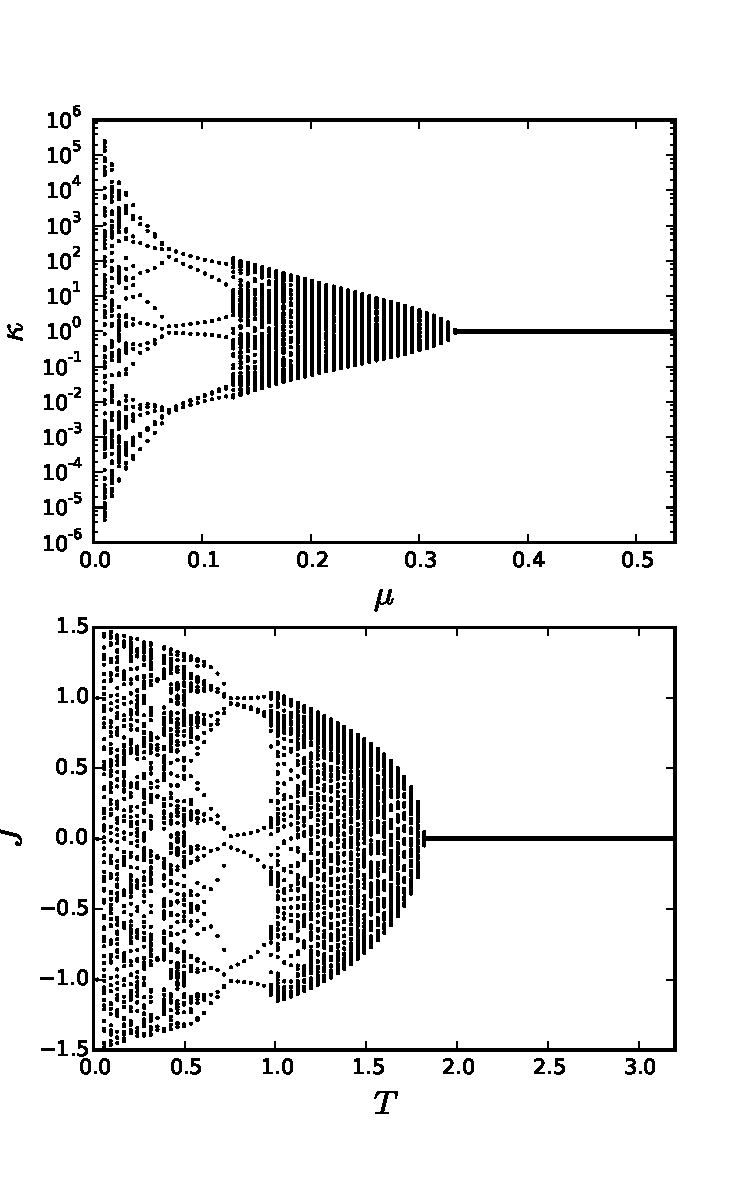
\includegraphics[width=0.6\columnwidth]{Chapter-3/HNNP_RG_Kvsmu_JvsT.pdf}
\protect\caption{ $\kappa$ and $J$ of HNNP RG recrusive numerical results. When $1/\mu < 1/3$ or $T < 2/\log(3)$, there is no stable fixed point. }
\label{fig:afm-hnnpkappa} 
\end{figure}


Similarly to the approach in HN3 and HN5, the Jacobian matrix of the recursive equations is
\begin{equation}
J_{11} = \frac{\partial \kappa'(\kappa, \lambda)}{\partial \kappa}=\frac{\lambda  (\mu +1)^2}{(\kappa  \mu +1)^2}-\frac{2 \kappa  \lambda  \mu  (\mu +1)^2}{(\kappa  \mu +1)^3}
\end{equation}
\begin{equation}
J_{12} = \frac{\partial \kappa'(\kappa, \lambda)}{\partial \lambda}=\frac{\kappa  (\mu +1)^2}{(\kappa  \mu +1)^2}
\end{equation}
\begin{equation}
J_{21} = \frac{\partial \lambda'(\kappa)}{\partial \kappa}=\frac{2 (\kappa +\mu ) }{(\kappa  \mu +1)^2}-\frac{2 (\kappa +\mu )^2 \mu }{(\kappa  \mu +1)^3}
\end{equation}
\begin{equation}
J_{22} = \frac{\partial \lambda'(\kappa)}{\partial \lambda}=0
\end{equation}
The 2 eigenvalues are 
\begin{eqnarray}
J_{\rm evig} = -\frac{(\mu +1)}{2 (\kappa  \mu +1)^3} \Big[\lambda  \mu  (\kappa +\kappa \mu -1)-\lambda \pm \nonumber \\ 
\sqrt{\lambda ^2 (\mu +1)^2 (\kappa  \mu -1)^2-8 \kappa  \left(\mu ^2-1\right) (\kappa +\mu ) (\kappa  \mu +1)} \Big] \nonumber \\
\label{eq:afm-hpeig}
\end{eqnarray}

\begin{figure}
\centering 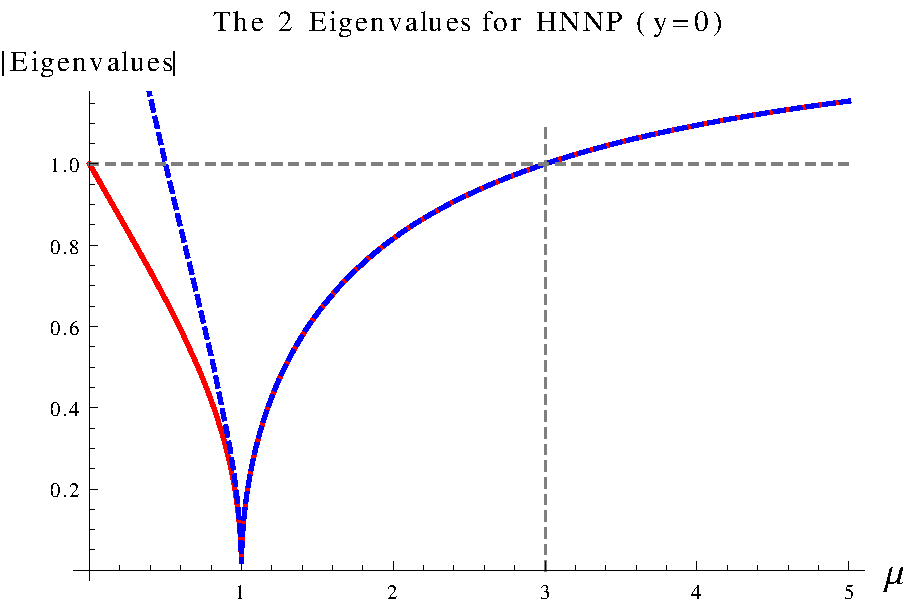
\includegraphics[width=0.6\columnwidth]{Chapter-3/HNNP_eigenvalues.pdf}
\protect\caption{The absolute values (1st norm) of the 2 complex eigenvalues for HNNP. For $0<\mu<1$, that is for the ferromagnetic case; while the antiferromagnetic region is $\mu>1$. You see the transition temperature is $\mu_g=3.0$ or $T_g=2/\log(3)=1.820478...$ because after that the $|{\rm eigenvalue}|>1$ . }
\label{fig:afm-hnnp_eigs} 
\end{figure}

\begin{figure}
\centering 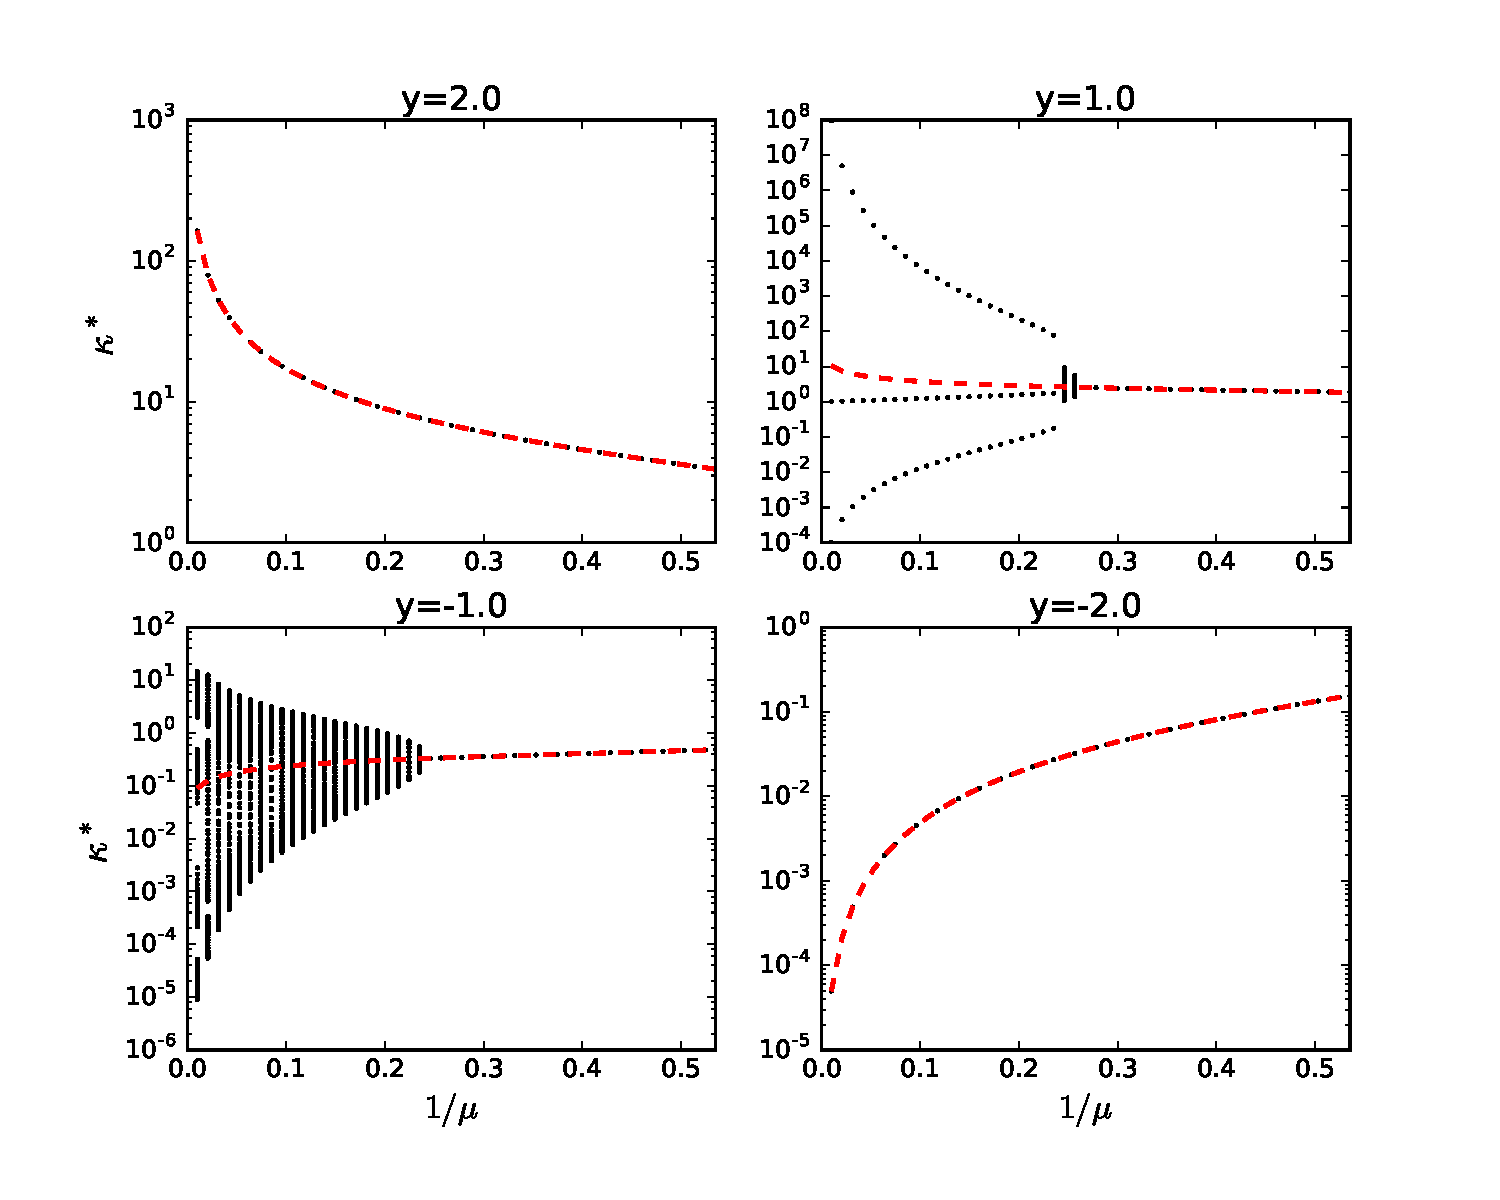
\includegraphics[width=1.0\columnwidth]{Chapter-3/HNP6_KvsMu_ys.pdf}
\protect\caption{Numerical iterations (dotted black) and analytical (red dashed) fixed points of $\kappa$. The numerical solutions are data points between RG steps $20,000$ and $20,100$. There is a chatoic transition for $-2.0<y<2.0$. }
\label{fig:afm-hp6Kys} 
\end{figure}

\begin{figure}
\centering 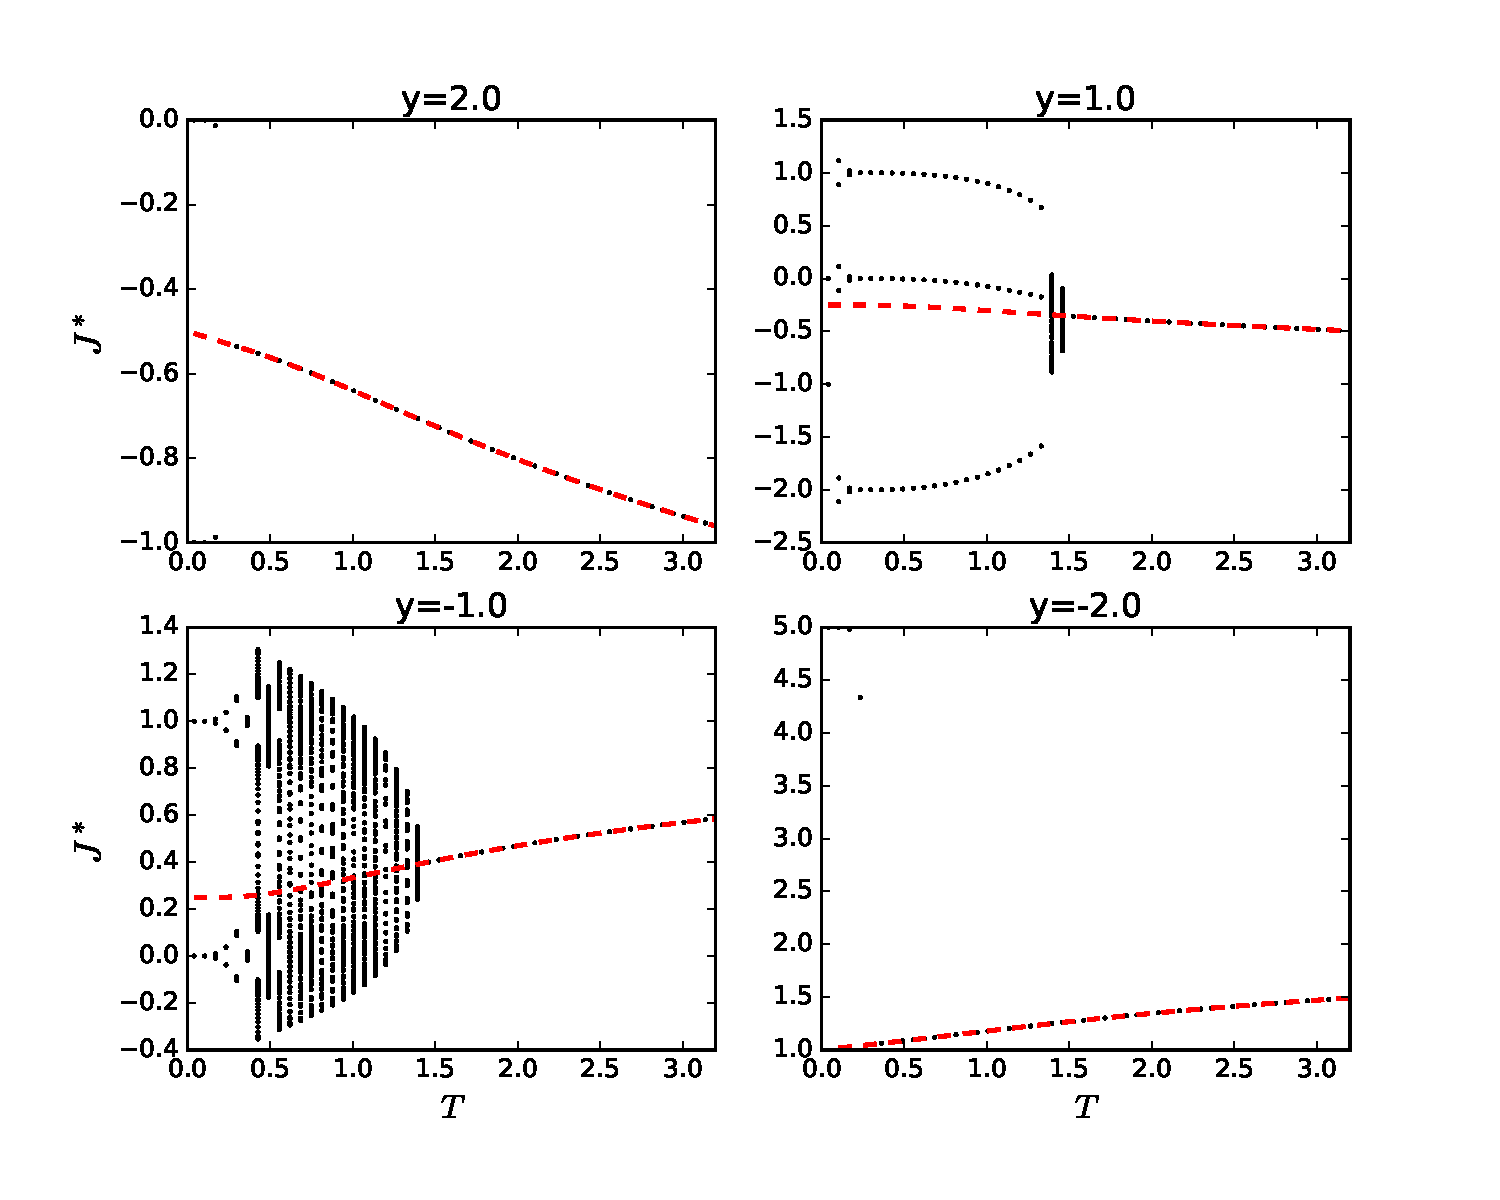
\includegraphics[width=1.0\columnwidth]{Chapter-3/HNP6_JvsT_ys.pdf}
\protect\caption{Numerical iterations (dotted black) and analytical (red dashed) fixed points of $J$. The numerical solutions are data points between RG steps $20,000$ and $20,100$. There is a chatoic transition for $-2.0<y<2.0$. At $y=\pm 2.0$, all the data points of numerical and analytical fixed points should exactly agree. The discrepancies at low temperatures is due to the finite numerical iterations. The discrepancies converge to 0 at infinite iterations which is to the thermodynamic limit.}
\label{fig:afm-hp6Jys} 
\end{figure}

We can plug in the 2 possible fixed points to these two eigenvalues, and the eigenvalues become
\begin{equation}
J_{\rm evig} = \frac{\pm \sqrt{-7 \mu ^2-2 \mu +9}-\mu +1}{2 \mu +2}
\label{eq:afm-hnnpJevig2}
\end{equation}
Because $\mu>1$ for AFM, the eigenvalues are complex numbers. In this case, the absolute values matter: if the absolute value is smaller than 1, there is a stable fixed points, otherwise there is not. The complex number means that the unstable fixed points are oscillating. More descriptions of the chaotic fixed points is included for generalized $y$'s later in this section. As shown in Fig. \ref{fig:afm-hnnp_eigs}, by solving the Eq. \ref{eq:afm-hpeig} $ ==1$, we can get the transition temperature is $\mu_g=3$ ($T_g=1.820478...$).


In this scenario, $y$ makes the fixed point much more complicated. One of the fixed point is
\begin{equation}
\kappa^* = 0, \ \ \lambda^* = \mu^{2+2y} 
\end{equation} 
Another positive fixed point for $\mu>1$ is 

\begin{equation}
\begin{array}{l}
\kappa^*=\frac{-2 \mu +\mu^{y/2}(\mu + 1) \left( \mu^{y/2}+\sqrt{4 (\mu -1) \mu +\mu ^y}\right) } {2 \mu ^2}  \\ \\
\lambda^* = \frac{1}{2} \mu ^{y-2} \left(2 (\mu -1) \mu +\mu ^y+\mu ^{y/2}\sqrt{4 (\mu -1) \mu +\mu ^y} \right) \\
\end{array}
\end{equation} 

Most interestingly, the fixed points are also chaotic for $-2<y<2$ (as shown in Fig. \ref{fig:afm-hp6Kys} and \ref{fig:afm-hp6Jys}).  When $y>2$, other links is relatively weak, and the model becomes fairly simple and has no phase transition. When $y<-2$, the whole system became similar to ferromagnetic model and have FM-like phase transitions (as shown in Fig. \ref{fig:afm-hp6KJnegy}). As shown in Fig. \ref{fig:afm-hp6KJnegy}, we can find the FM-like transition temperatures by solving $\kappa^*==0$  for $y<-2.0$, which is equivalently the solutions of 
\begin{equation}
1 - \mu^{1 + y} - \mu^{2 + y} = 0 
\end{equation}


\begin{figure}
\centering 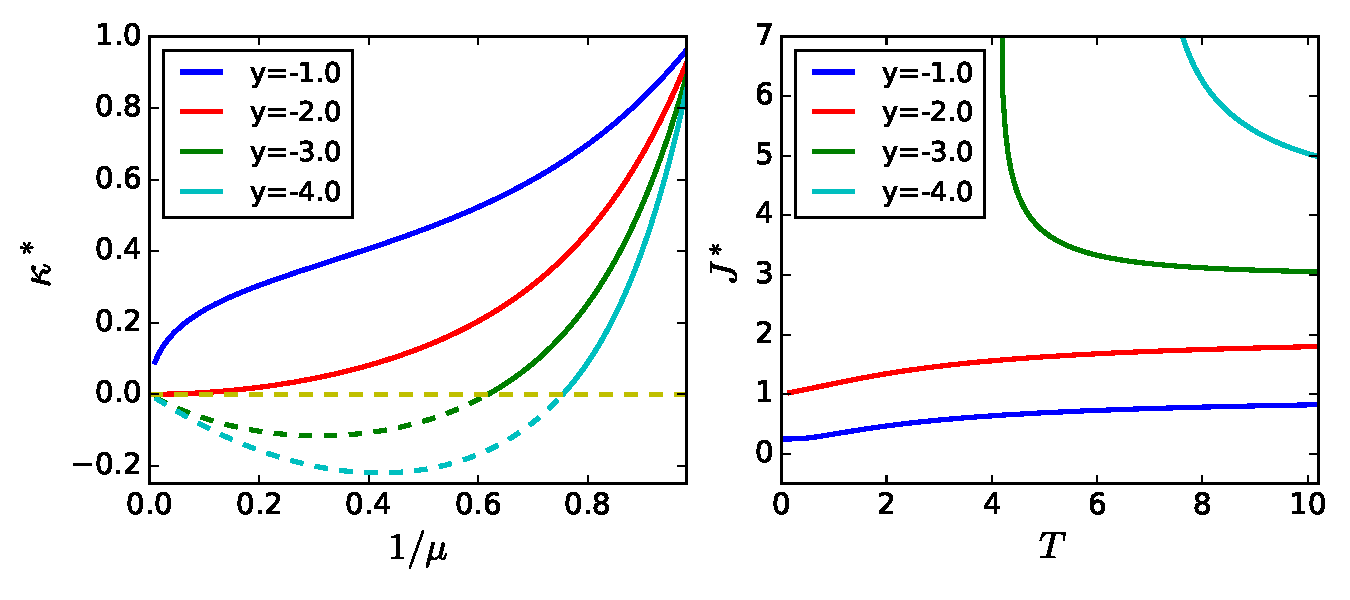
\includegraphics[width=1.0\columnwidth]{Chapter-3/HP_KJvsTys_FMTrans.pdf}
\protect\caption{Analytical (red dashed) fixed points of $\kappa$ and $J$ with different $y$'s. The solid curves are real and positive fixed points; while the dashed curves are negative ones. The 0 fixed points is the FM-like transition points.}
\label{fig:afm-hp6KJnegy} 
\end{figure}

\begin{figure}
\centering 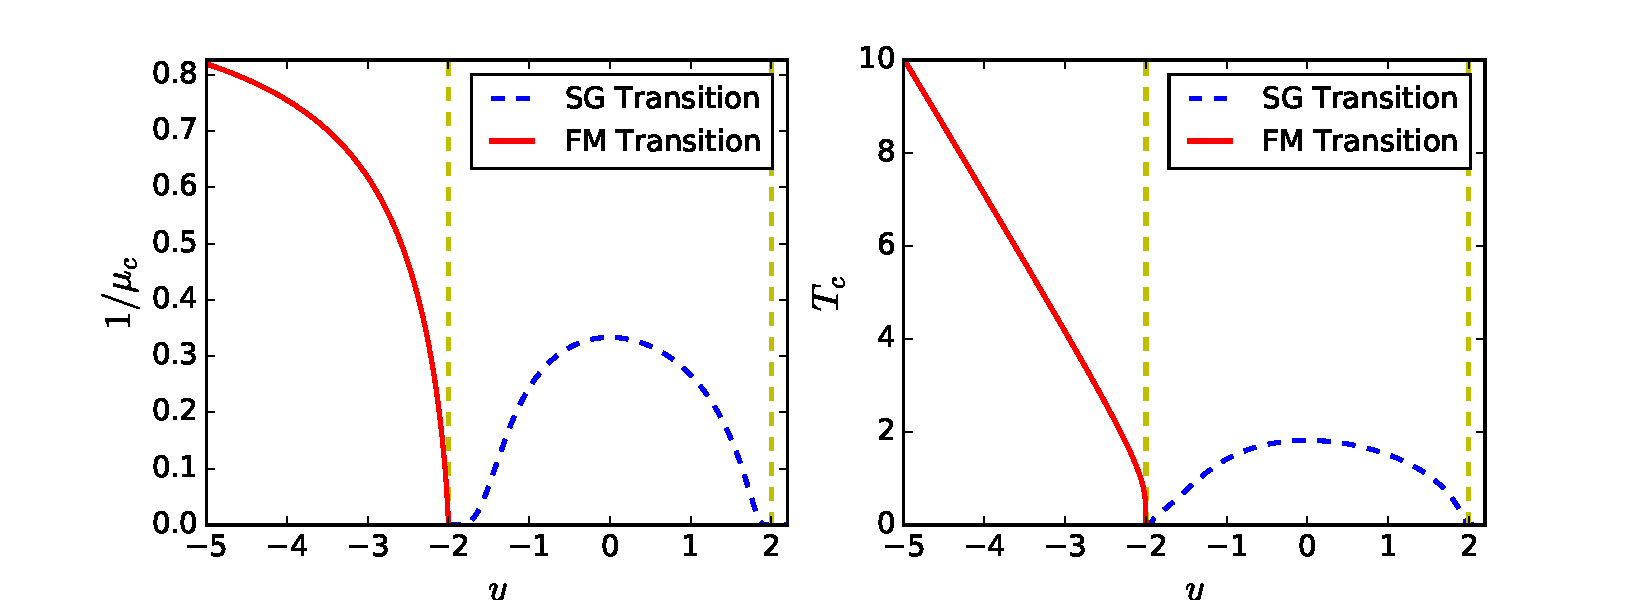
\includegraphics[width=1.0\columnwidth]{Chapter-3/HN6_TransTvsY1.pdf}
\protect\caption{Numerical Solution of chaotic transition temperatures and phase transition temperatures at different $y$'s for HNNP and HN6 interpolations. }
\label{fig:afm-hp6Tys} 
\end{figure}

The chaotic transition temperatures $T_g$ can be determined from the eigenvalues of the Jacobian matrix.
The Jocobian matrix is
\begin{equation}
J_{11} = \frac{\partial \kappa'(\kappa, \lambda)}{\partial \kappa}=\frac{\lambda  (\mu +1)^2}{(\kappa  \mu +1)^2}-\frac{2 \kappa  \lambda  \mu  (\mu +1)^2}{(\kappa  \mu +1)^3}
\end{equation}
\begin{equation}
J_{12} = \frac{\partial \kappa'(\kappa, \lambda)}{\partial \lambda}=\frac{\kappa  (\mu +1)^2}{(\kappa  \mu +1)^2}
\end{equation}
\begin{equation}
J_{21} = \frac{\partial \lambda'(\kappa)}{\partial \kappa}=\frac{2 (\kappa +\mu ) \mu ^{2 y}}{(\kappa  \mu +1)^2}-\frac{2 (\kappa +\mu )^2 \mu ^{2 y+1}}{(\kappa  \mu +1)^3}
\end{equation}
\begin{equation}
J_{22} = \frac{\partial \lambda'(\kappa)}{\partial \lambda}=0
\end{equation}

The transition temperature can be solved by setting an equation of $\rm |eigenvalue|==1$. The explicit equations of the eigenvalues are not shown due to length and complexity. Because the 2 eigenvalues are conjugate complex numbers, $\rm |eigenvalue|$ is the 1st norm. For complex eigenvalues, if the 1st norm is smaller than 1, the recursive equations can reach a stable fixed point; otherwise, it would not. Also, complex eigenvalues usually mean oscillating flow of the parameters, which is what we see in the numerical iterations in Fig. \ref{fig:afm-hp6Kys}.
The equation of $\rm |eigenvalue|==0$ is not solvable analytically but can be numerically solved to find the chaotic transition temperatures. The transition temperatures at different $y$'s are shown in Fig. \ref{fig:afm-hp6Tys}




\subsection{Equilibrium Properties}
\label{sec:afm-eqa}
Equilibrium properties are vital to learn critical phenomena and almost impossible to study experimentally for glassy systems due to the extremely long relaxation. To learn the equilibrium properties of AFM in Hanoi networks, there are 2 methods: Wang-Landau sampling and/or RG. 

\begin{figure}
\centering 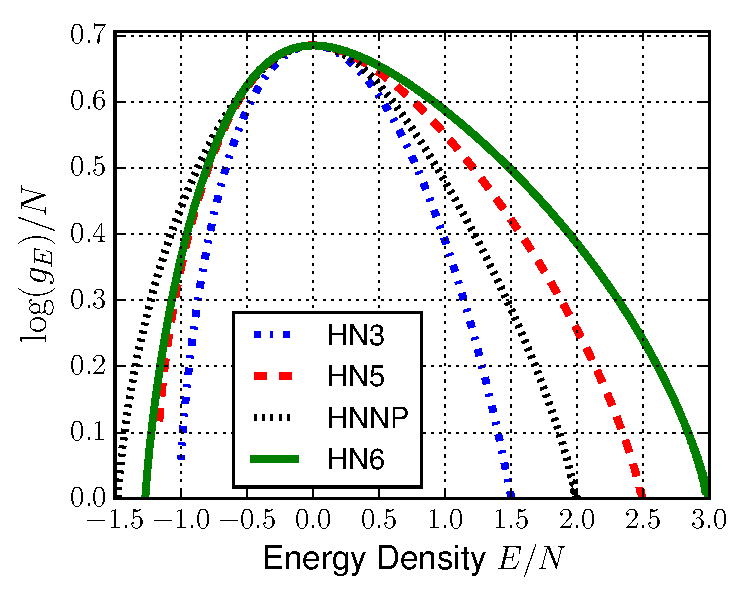
\includegraphics[width=0.6\columnwidth]{Chapter-3/HN35P6DOS_h3.pdf}
\protect\caption{Density of states from Wang-Landau sampling for system size $N=512$. Both the planar networks have highly degenerated ground states; while the nonplanar ones have unique ground states. This is also confirmed by the entropy from RG. }
\label{fig:afm-doswl} 
\end{figure}

Wang-Landau sampling can estimate the density of states $g_E$, which yields the partition function as 
\begin{equation}
Z(\beta)=\sum_{i=1}^{N_{E}}g_{E_i}e^{-\beta E_i}
\end{equation}
where $\beta$ is $1/T$, and $N_E$ is the total number of energy states. The density of states for different HNs in AFM are shown in Fig. \ref{fig:afm-doswl}. We can see there is clearly a difference between planar (HN3, HN5) and nonplanar networks (HNNP, HN6). The planar networks have highly degenerate ground states, which may indicate more glassy dynamics at low temperature. The nonplanar networks have unique ground state, which may indicate an equilibrium phase transition. The ground states degenency can be further proved by the entropy density $s$ from RG as shown in Fig. \ref{fig:afm-entropy}. However, the Wang-Landau sampling can only converge for system sizes $<1024$. Due the small system sizes in Wang-Landau sampling's results, no evidence is obtained to prove the speculations of phase transitions.
Therefore, RG is needed to reach any meaningful conclusion for systems in the thermodynamic limit.

\begin{figure}[h]
\centering 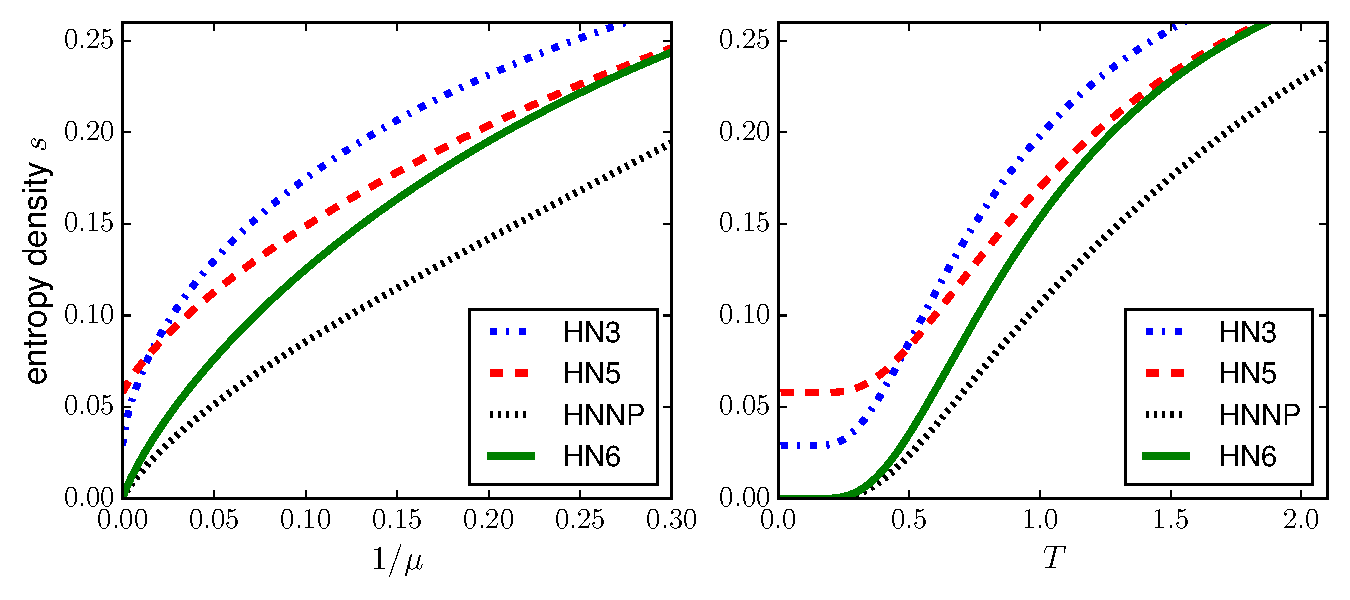
\includegraphics[width=0.88\columnwidth]{Chapter-3/HNs_entropy_density.pdf}
\protect\caption{Entropy Densities for all HNs of system sizes $N=2^{16}, 2^{32}, 2^{64}$. Each Hanoi network has 3 curves of different system sizes, and these curves all cllapses on each other, which shows these curves can represent the behavior in the thermodynamic limit.  }
\label{fig:afm-entropy} 
\end{figure}

\begin{figure}[h]
\centering 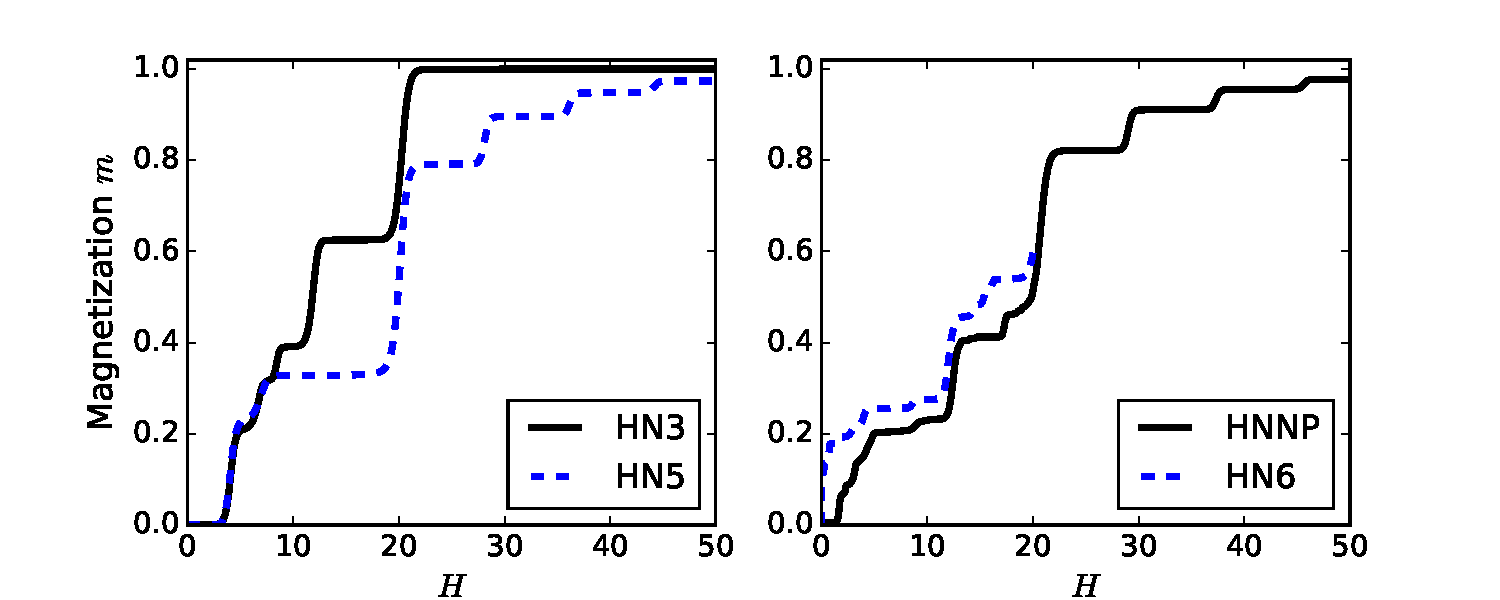
\includegraphics[width=0.9\columnwidth]{Chapter-3/HNs_MagvsH_m_vs_H.pdf}
\protect\caption{Magnetization patterns with increasing external magnetic fields at low temperature $T=0.1$ for system size $N=2^{128}$ using RG.}
\label{fig:afm-magplt}
\end{figure}

Using RG, we explored most common physical properties, such as internal energy per spin $\langle e\rangle$, magnetization per spin $\langle e\rangle$, free energy $\langle e\rangle$ with different boundary conditions, specific heat, susceptibility. Our interesting findings are described as follows.

The results of the internal energy have been included in Sec. \ref{sec:afm-dyn} and show the glassy dynamics ( Fig. \ref{fig:afm-hnsjam} ) sand the power-law relaxation (Fig. \ref{fig:afm-hnsscaling}). 

Another interesting finding is the magnetization behavior as to the increasing external
 magnetic field. The plateau patterns similar to others' findings \cite{ohanyan2003mag} have
 been found as shown in Fig. \ref{fig:afm-magplt}. These plateaus may be because of the
 hierarchically distributed local spin pattern. Specifically, the overall average magnetization per
 spin is zero, but the local spin-generated fields are non-zero and may be correlated with the
 Hanoi networks' hierarchy. These local non-zero fields may have a nonuniform discrete
 distribution, which leads to the plateaus with different lengths. Often, these magnetization
 plateaus are believed to be from quantum effects 
\cite{kageyama1999pleatu, kageyama2000direct}. This result provides another example of
 classical system where the plateaus are mainly caused by the structure of the networks. 
Further conclusion needs detailed information of the low-temperature (even ground states)
 spin configuration, which is not directly retrievable from RG.

\begin{figure}
\centering 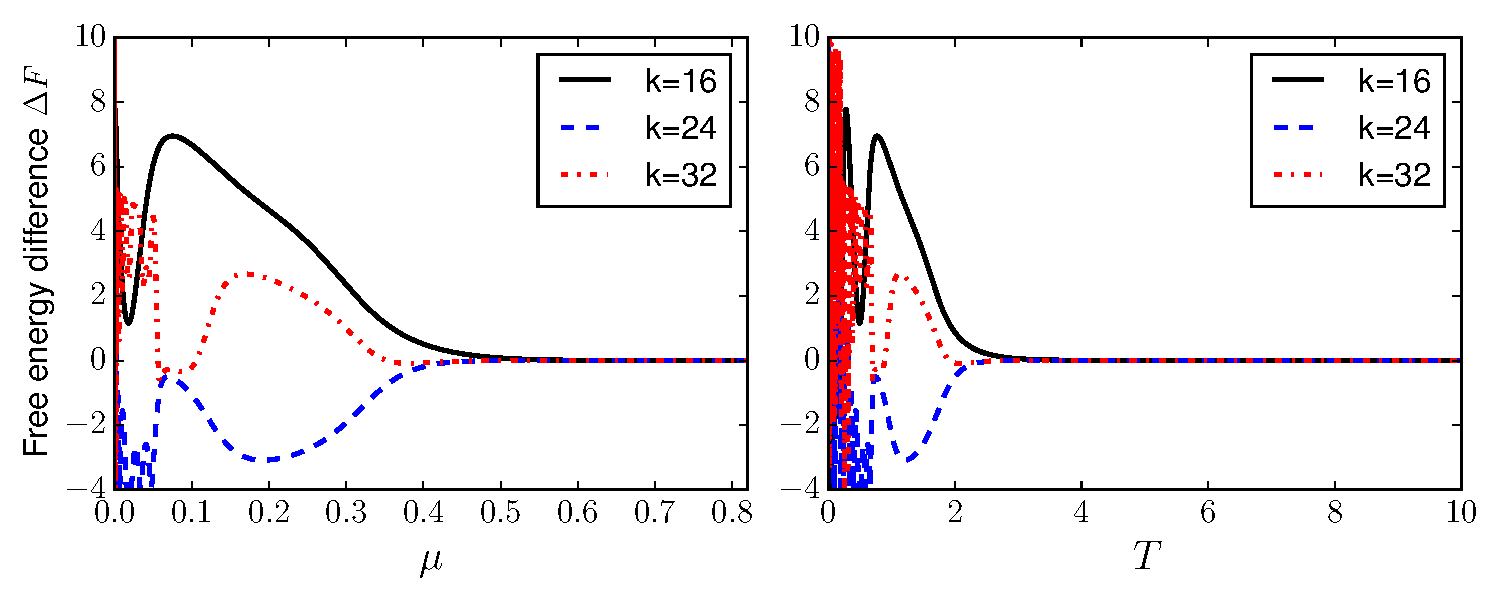
\includegraphics[width=1\columnwidth]{Chapter-3/freeE_lowT2highT.pdf}
\protect\caption{The free energy difference between the 2 boundaries conditions at different temperatures. The system size is $N=2^k$, which are $2^{16}$, $2^{24}$, $2^{32}$ in the figure above. Obviously, at higher temperatures, there is no difference; at low temperatures, there is more and more difference variations for bigger and bigger system sizes. A plot for low $T$ is shown next (Fig. \ref{fig:afm-freeEdiff}) which shows the chaos at low $T$.  }
\label{fig:afm-freeEdiff_allT} 
\end{figure}

One of the main goals of RG is to explore the chaotic behaviors found in the fixed point analysis.
 In AFM, the free energy with different boundary conditions has been used to study the chaos in physical systems. The reference parameter is the free energy difference $\Delta F$ (Eq. \ref{eq:afm-freediff}) between different boundary conditions. The difference at a wide range of temperatures are shown in Fig. \ref{fig:afm-freeEdiff_allT} which shows the $\Delta F$ is 0 at high $T$ but non-zero and chaotic at low $T$. The curves may have very different patterns for difference system size, and Fig. \ref{fig:afm-freeEdiff}  is an example. 

\begin{figure}
\centering 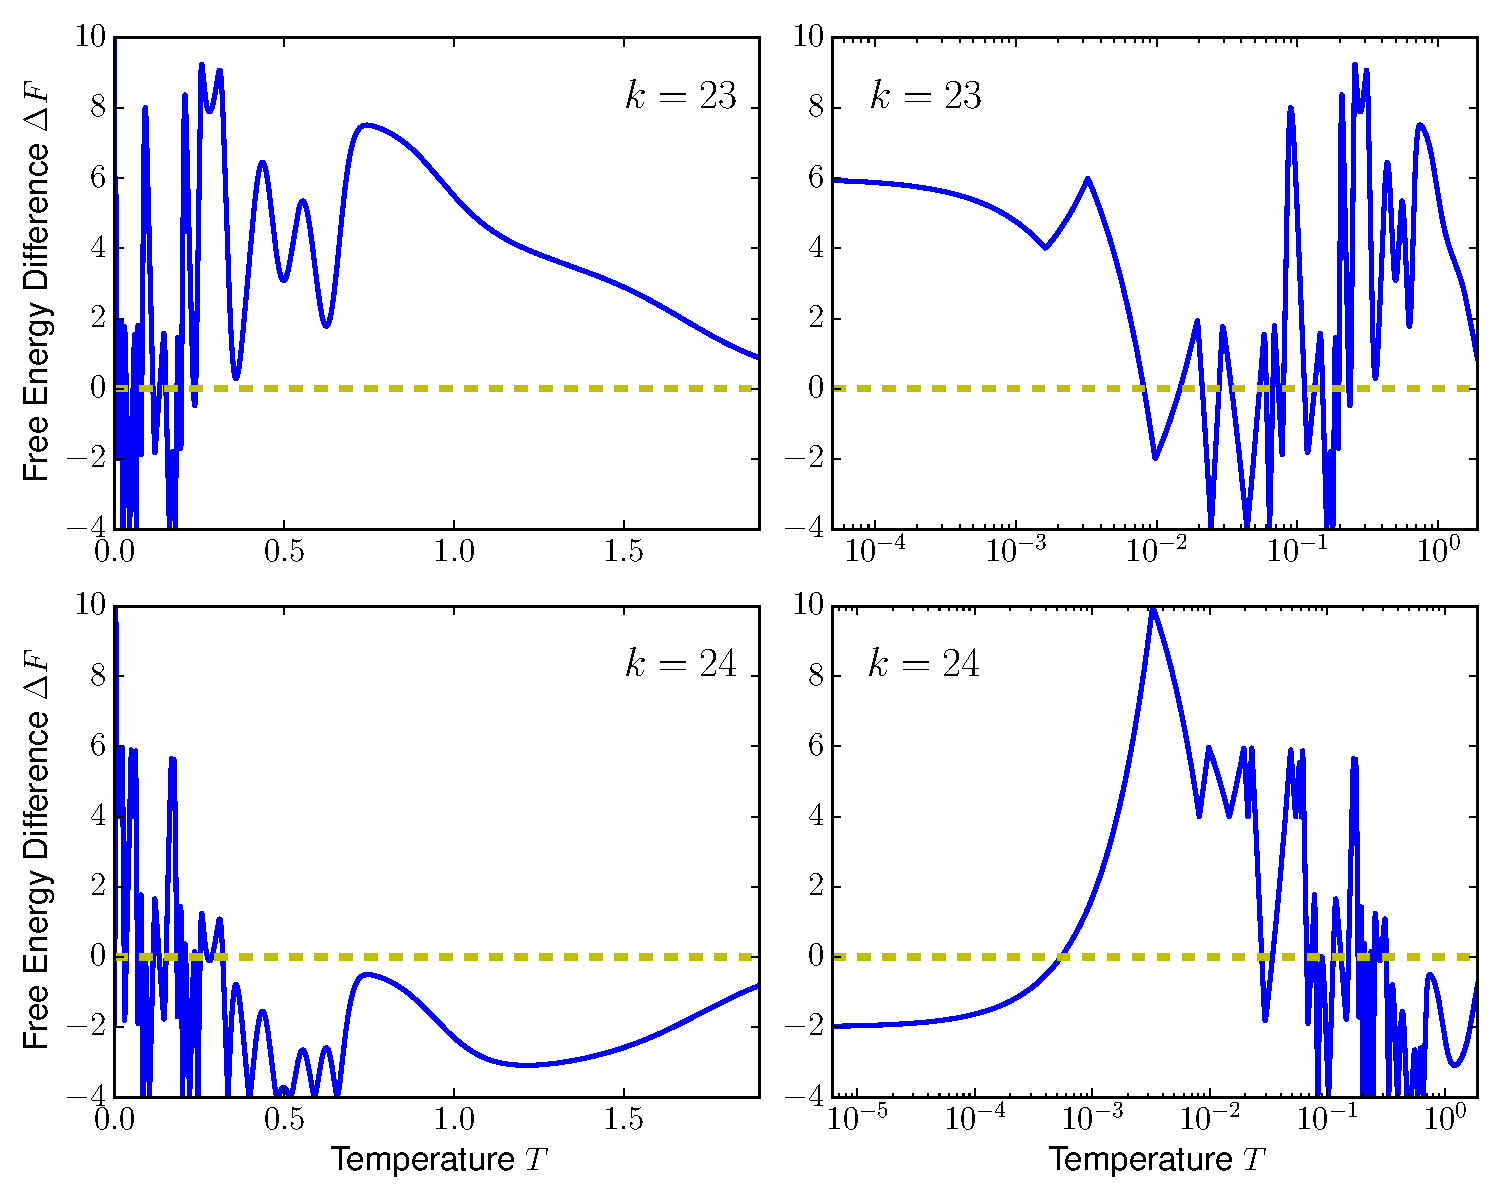
\includegraphics[width=0.8\columnwidth]{Chapter-3/freeEdifference_k23_24.pdf}
\protect\caption{The free energy difference between the 2 boundaries conditions at low temperatures $T<2.0$. The yellow dashed line is to show where the crossings of $f_1$ and $f_2$ are. ($f_1$: parallel boundary condition; $f_2$: anti-parallel boundary condition.) }
\label{fig:afm-freeEdiff} 
\end{figure}

\begin{figure}
\centering 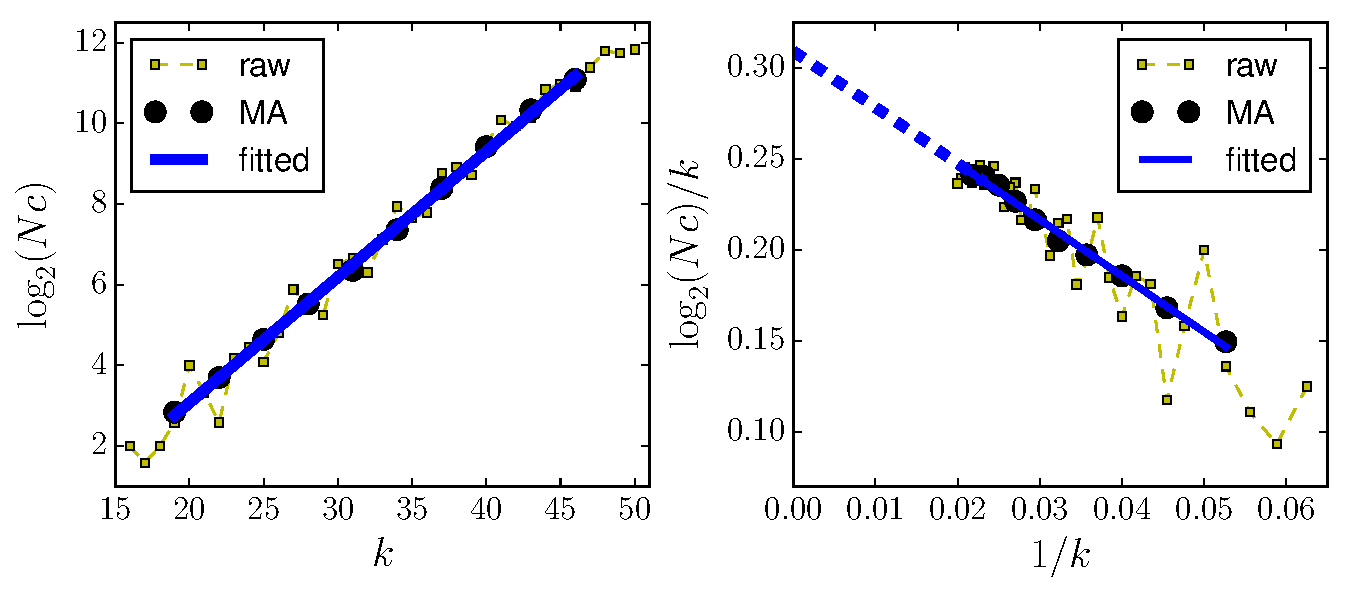
\includegraphics[width=0.8\columnwidth]{Chapter-3/chaotic_exponents_freeE_binning.pdf}
\protect\caption{Number of free energies crossings fitted to $k$ (=$\log_2 N$) in the temperature range $T \in [10^{-3}, T_g]$ for HNNP. The yellow squares are the raw $N_c$'s which have fluctuations due to finite size scaling and numerical precision. To get a more reliable fitting, the moveing average (black circles) with window size of 6 and overlap of 3 are used for fitting. Two methods of fitting are used: Eq. \ref{eq:afm-fit1} (left figure) and Eq. \ref{eq:afm-fit2} (right figure). The exponents are $0.312\pm 0.003$ and $0.309 \pm 0.003$, respectively. Both of the $R^2$ is bigger than $0.99$.}
\label{fig:afm-freeEfit} 
\end{figure}

The crossing point is where $\Delta F = 0$ and $\Delta F$ changes sign. In other words, $f_1$  (parallel boundary condition) and $f_2$ (anti-parallel) switch their order. In a spin glass with chaotic dynamics, the number of crossings $N_c$ is expected to increase polynomially with system size 
\begin{equation}
N_c = A N^\alpha
\end{equation}
where $A$ is a constant, $N$ is the system size, and $\alpha$ is the exponent. The exponent $\alpha$ is called chaotic exponent. There is two way to obtain chaotic exponent $\alpha$. The first way is 
\begin{equation}
\log_2 N_c = \log_2 A + \alpha \log_2 N
\label{eq:afm-fit1}
\end{equation}
, and the second way is 
\begin{equation}
\frac{\log_2 N_c }{\log_2 N } =\frac {\log_2 A }{\log_2{N}} + \alpha 
\label{eq:afm-fit2}
\end{equation}
where $\log_2 N = k$. The two ways can show us the trend from different perspectives as shown in Fig. \ref{fig:afm-freeEfit}. 
These two exponents are $0.312\pm 0.003$ and $0.309 \pm 0.003$, respectively. Both strongly show there is a power-law increase with system size. 

As you may notice from the free energy curves in Fig. \ref{fig:afm-freeEdiff}, $N_c$ may dependent on the temperature and step size. First, we tested different 2 more temperatures ranges $T \in [0.1, 0.2]$ and $T \in [0.2, 0.3]$ which show similar pattern. Second, different step sizes are tested to make sure the $N_c$ does not change with a smaller step size. 


\section{Summary and Conclusion}



\chapter{Aging in the Two-Dimensional Random Field Ising Model}
\label{chap-rfim}
The work in this chapter is motivated by the experimental study of antiferromagnet CoO polycrystalline films in Sergei Urazhdin's group \cite{ma2016prb}. In the experimental findings, glassy dynamics and non-Neel-Arrhenius aging has been discovered. In this computational study, a Monte Carlo simulation using the Random Field Ising Model (RFIM) is proposed to explain and understand the experimental findings.

This chapter first introduces RFIM and its connection with the experiment. Then the details of Monte Carlo simulations are described, and the choices of parameters are discussed. All the results from simulations  are shown in the third section (Sec. \ref{sec:rfim-results}). Finally, we conclude this chapter with interesting findings and discussions.
 
\section{Random Field Ising Model and experiments }
\label{sec:rfim-model}
As introduced in Sec. \ref{sec:intro-rfim}, the RFIM has been extensively utilized for modeling diluted antiferromagnets \cite{fernandez1988random}, impure substrates \cite{villain1982commensurate}, and magnetic alloys \cite{fisher1988theory}. The experimental system to simulate in this work is the polycrystalline films of antiferromagnet CoO \cite{ma2016prb}. It has 2 layers, antiferromagnet (AF) CoO layer with thicknesses from 2nm to 10nm and ferromagnet (F)10-nm-thick Py layer. The resistance is measured at low temperatures to investigate the aging behaviors. A power-law scaling is observed in the aging, which is inconsistent with the Neel-Arrhenius model of thermal activations. Urazhdin, {\it et. al.} \cite{ma2016prb} believe the phenomena indicate cooperative aging and may  provide new insights into the mechanisms of AF/F bilayers, and potentially other frustrated magnetic systems.


To simulate this complex experimental system,  we need to make several simplifying approximations. First, we are interested in the aging phenomena in the AF layer, and therefore model only this layer. We assume that the magnetization state of the thin AF film does not vary through its thickness, so that it can be approximated by a two-dimensional (2d) square lattice of Ising spins. We consider the staggered AF order parameter, which is modeled by the ferromagnetic exchange interaction of each spin with its four nearest neighbors. The dipolar spin-spin interactions and the interaction with the modest external fields used in our experiments are negligible. The exchange interaction with F layer is described by an uncorrelated quenched random field $h$ with a Gaussian distribution $\mathcal{N}(0,\sigma_{\text{rand}}^{2})$ of zero mean and width $\sigma_{{\rm rand}}$. In this approximation, the reversal of the magnetization of F utilized in our experiments to initiate aging is modeled by the reversal of the random field.

The direct comparison between experimental material and simulational system is described as follows. The freshly prepared sample is coarse-grained to a two dimensional (2D) RFIM with a random spin initialization.  To obtain a stable magnetic state, the samples are cooled from $T=300K$ at a rate of $4K$ per minute to  low temperatures of $5K \sim 150K$ for aging; while, in the simulation, a similar approach is taken to anneal the system slowly to a stable state from $T=10$ to a certain low temperature ($0.1<T<1.0$). In the experiment, the aging is captured by measuring the resistance changes with time under flipping external magnetic field $H$. The flipping field $H$ is to keep the system in a measurable aging state. In the simulation, the energy relaxation is measured with flipping random fields, i.e. changing the sign of the random fields.

The random field Ising model, for example, in a square lattice, is described by the Hamiltonian is
\begin{equation}\label{energy}
\mathcal{H}=-J\sum_{<i,j>}s_{i}s_{j}-\sum_{i=1}^{N=L^{2}}h_{i}s_{i}
\end{equation}
where the coupling constant $J$ sets the overall energy scale and
is set to $1$ here, the spins are bimodal, $s_{i}=\pm1$, where $
\langle i,j \rangle$
enumerates nearest-neighbor spins,  $L$ is the linear dimension of the 2D square lattice with the total number of spins $N=L^{2}$, and periodic boundary conditions. The effects of temperature are modeled by the sequential random flipping of spins with the probability $P=\exp(-\Delta E/T)$ where $\Delta E$ is the energy change if the flipping is committed. The time $t$ is measured in sweeps, where one sweep corresponds to $N$ random sequential update attempts.  

The experimental system and connection with random field Ising model has been described and discussed in this section. The next section covers more details of the simulation.


\section{Monte Carlo Simulation}
The general procedure of MC simulation in RFIM is similar to that in Chapter \ref{chap-afm}, but the most challenging part is to approximate the experimental system with a reasonable set of procedures and parameters. Different procedures are tested to simulate the experimental procedure, and the final procedure used in the simulation is shown in the end of this section. Meanwhile, a wide range of parameters are also tested to explore the dynamics and behaviors of the RFIM, and all the parameters tested are shown in Table \ref{table:rfim-paras}. 

\begin{table}[h!]
\begin{center}
\begin{tabular}{l | r}
Variables              & Parameters \\
\hline
Temperature $T$ 	& 	$0.1 \sim 1.0$   \\
Random Field $\sigma_\text{rand}$            &		 0.1, 0.3, 0.5, 1.0   \\
Annealing rate $r$          & 	1e-1, 1e-2, 1e-3, 1e-4, 1e-5   \\
System Size $N$ 	&	  $32^2$, $64^2$, $128^2$, $256^2$   \\
MC sweeps in each cycle  	&	  $2,000 \sim 50,000$   \\
\end{tabular}
\end{center}
\caption{Parameters tested in the simulations.}
\label{table:rfim-paras}
\end{table}

In the simulation, we first anneal the system to the aging temperature $T$ at a slow rate of $r=0.0001$ per Monte Carlo sweep, which is comparable to the cooling process in the experiment. After the annealing, the system stops evolving at some metastable state with spin domains (as shown in Fig. \ref{fig:rfim-baaneal}). The snapshots before and after annealing is shown in Fig. \ref{fig:rfim-baaneal}. Then we simulate the aging at a fixed aging $T$ ($0.1\le T \le 1.0$). In the aging process, we flip the random fields every 20,000 MC sweeps, which excites the system to a non-equilibrium state. The parameters used in the simulations are determined by exploring a wide range of each parameter (see Table \ref{table:rfim-paras}). For example, annealing rates $\left( 10^{-1} \le r \le 10^{-5}\right)$ are tested to make sure that a metastable state is reached, and slower annealing rates lead to no significant changes to the metastable state. Another important parameter is the random field standard deviation $\sigma_{\rm rand}$ where too small $\sigma_{\rm rand}$ leads to plain 2D Ising model with exponential relaxation, and too big $\sigma_{\rm rand}$ would dominate the spin behavior comparing to unit near-neighbor spin interactions. 

\begin{figure}
\centering 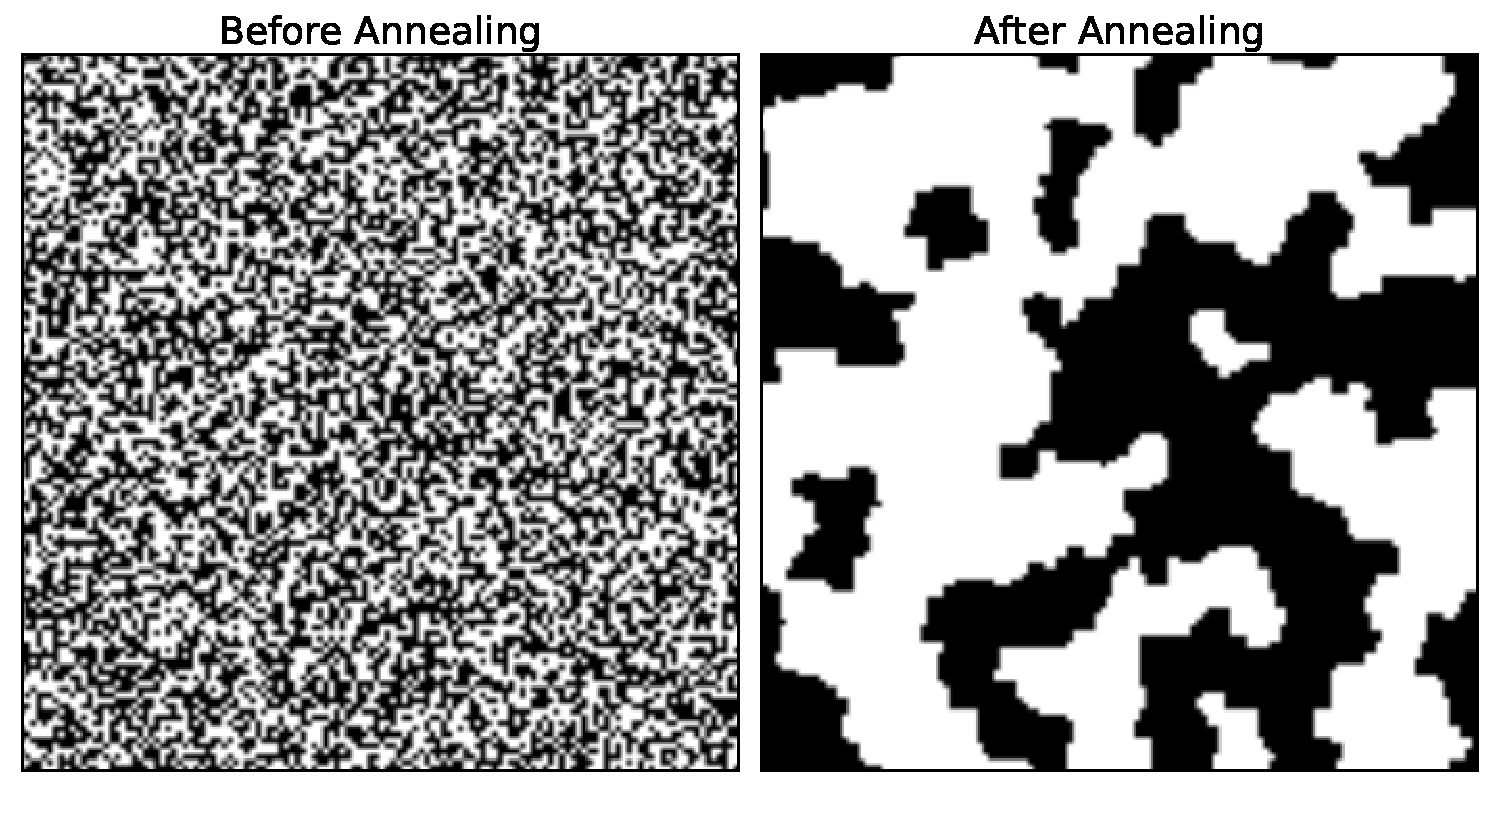
\includegraphics[width=0.9\columnwidth]{Chapter-4/RFIM_Before_After_Annealing}
\protect\caption{The snapshots of spin configurations before and after annealing of system size $L=128$. The state before annealing is simply a random state; while the state after annealing is a metastable state which seemingly does not change any more.}
\label{fig:rfim-baaneal} 
\end{figure}


After exploring different procedures and different parameters, the final procedure and parameters used in the simulation are
\begin{enumerate}
\item Randomly generate independent and identically distributed (i.i.d.) random field ($h_i\sim  \mathcal{N}(0, 1)$) and a random spin orientation ($s_i=\pm1$) for each site;
\item Anneal the system from temperature $T_0=10$ to the aging $T$ ($T=0.1\sim 0.5$) at a rate of $r=10^{-4}$, and the spins are randomly flipped using Metropolis choice based on the energy change;
\item After annealing to a certain temperature, fix the aging temperature $T$  ($T=0.1\sim 0.5$), flip the spins using Metropolis choice, and measure the energy relaxation;
\item Flip the random fields every $20,000$ MC sweeps after the annealing to keep the aging measurable in a reasonable time length.
\end{enumerate}

The results from simulation and their comparison to experiments are described in the next section below.


\section{Results and Comparison to Experiments}
\label{sec:rfim-results}
\begin{figure}
\centering 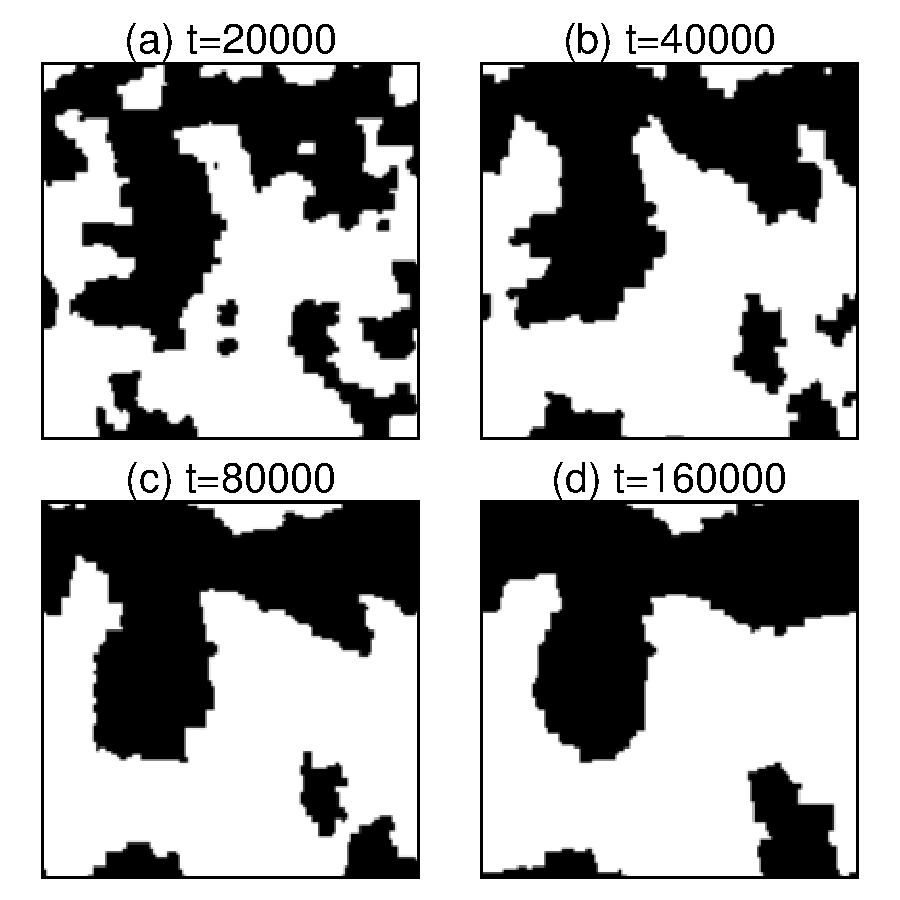
\includegraphics[width=0.8\columnwidth]{Chapter-4/spin_plot1_Norf}
\caption{Spin pattern snapshots in the Monte Carlo simulation at $T=0.3$ for the system size $L=128$. (a) is the spin pattern after the annealing and before the first random filed. (b), (c), and (d) are the spin snapshots at the end of cycles 1, 3, and 7, respectively. The corresponding energy changes can be found in Fig. \ref{fig:rfim-Es1}. In the aging process, there is clearly domain wall formed gradually. }
\label{fig:rfim-spinshots}
\end{figure}

\begin{figure}
\centering 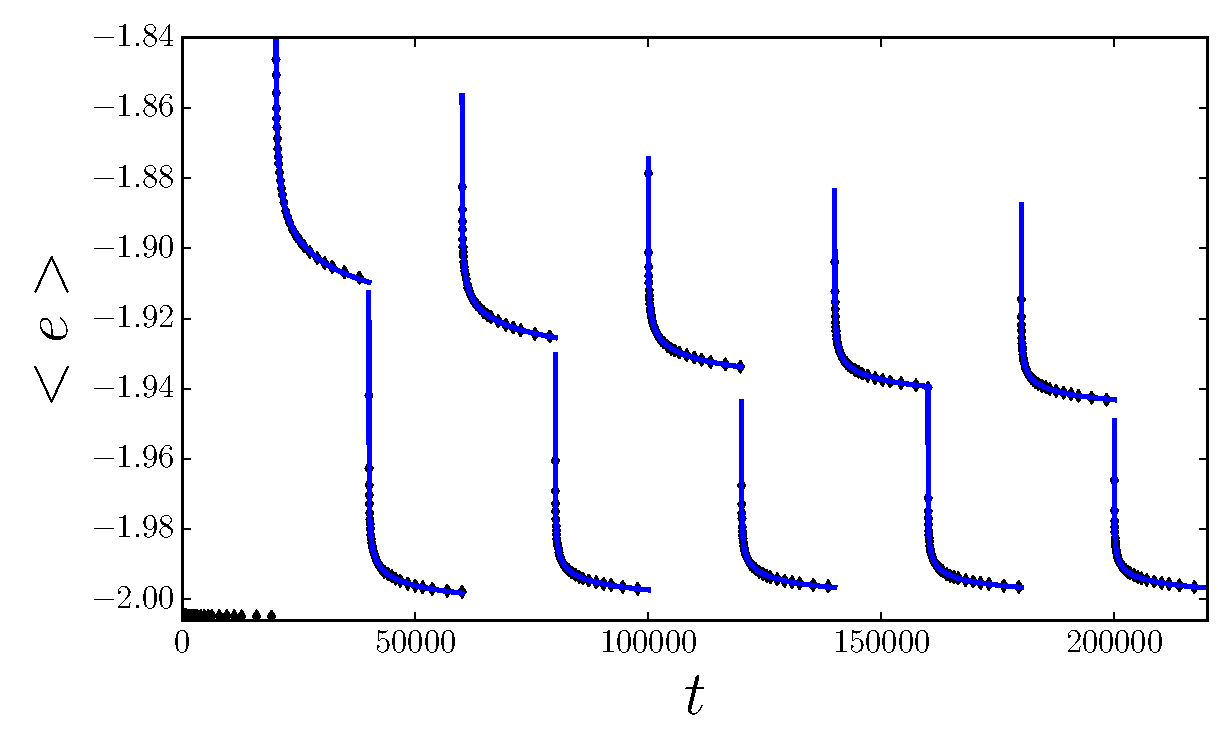
\includegraphics[width=0.8\columnwidth]{Chapter-4/Energy_simultion_fitted_10cycles_T03} 
\caption{Sequential simulations of energy relaxation for the system size $L=128$ with
random field $\sigma_{\text{rand}}=1.0$, temperature $T=0.3$. Black symbols represent an average of 100 simulation runs, and the blue curves are the power-law fittings with Eq.~(\ref{eq:rfim-fit}). Each individual simulation is performed starting with the initial state obtained by quasi-adiabatic annealing.}
\label{fig:rfim-Es1} 
\end{figure}

After the annealing, the system reaches a metastable state with interlocking spin domains of oppositely oriented spins. Although almost all spins are aligned with their neighbors at the end of annealing and attain their Ising-energy per spin, $\left\langle e\right\rangle \approx-2$,
see Fig.~\ref{fig:rfim-spinshots} and \ref{fig:rfim-Es1}, a sub-extensive amount of energy remains stored in rough domain walls that are pinned by the random field. To initiate aging at a fixed temperature $T$, we flip the random fields and simulate the evolution over 20,000 steps, after which the random field is flipped again and the simulations are repeated. The field flip brings the system into a non-equilibrium state, dislodging the domain walls. The snapshots of the spin distributions taken in the end of different aging cycles in Fig. \ref{fig:rfim-spinshots} show evolving spatial patterns, indicating that the system does  not relax to a unique equilibrium state, consistent with the experimental result \cite{ma2016prb}.

To establish the correlation with our experimental observations, a wide range of values (as shown in Table \ref{table:rfim-paras}) was explored for each parameter. For example, we tried the random field $\sigma_{\text{rand}}$ from $0.1 \sim 2.0$ where we found that small random fields would behave similarly as 2D Ising model, and big random fields would be dominate comparing to $J$. The measured variations of magneto-resistance due to aging are directly proportional to the variations of the local random field exerted by AF on F.  

\begin{figure}
\centering 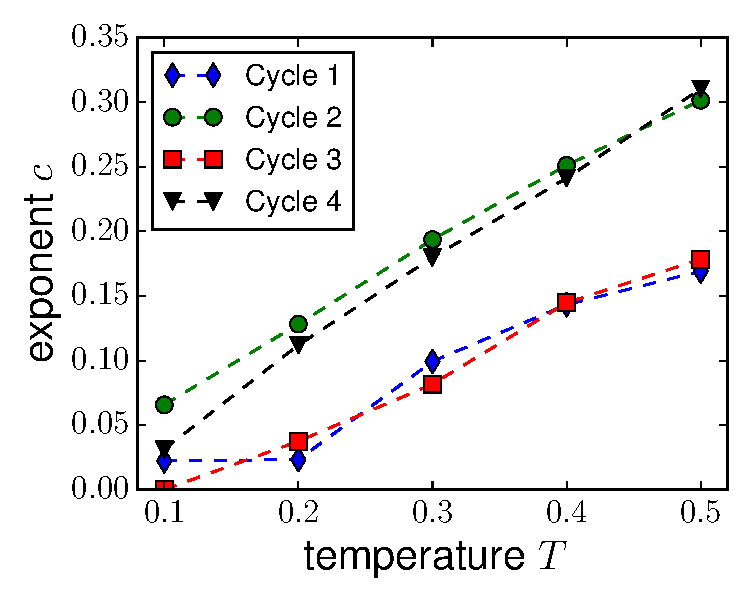
\includegraphics[width=0.5\columnwidth]{Chapter-4/exponent_scale_4cycle_T03}
\protect\caption{Dependence of exponent $c$ on temperature, for the system size $L=128$ with random field $\sigma_{\text{rand}}=1.0$. At low temperatures, the power-law fitting may not converge sometimes, for example, in Cycle 3 at $T=0.1$. That is also why no temperatures $T<0.1$ is used in the simulations. }
\label{fig:rfim-expT} 
\end{figure}

\begin{figure}
\centering 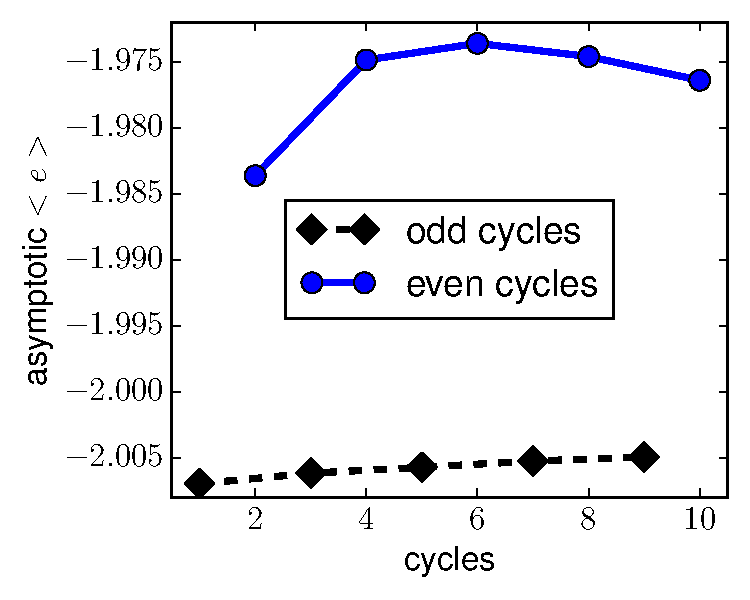
\includegraphics[width=0.5\columnwidth]{Chapter-4/asymptotic_E_T03_10cycles}
\protect\caption{Asymptotic energy for different aging cycles for system size $N=128^2$ at temperature $T=0.3$. The asymptotic energy is obtained from the power-law fitting at $t\rightarrow\infty$, i.e. $e_0$ in Eq \ref{eq:rfim-fit}. Other temperatures tested show the same pattern.} 
\label{fig:rfim-asm}
\end{figure}

To compare the results of our simulations to the experimental observations, we analyzed the evolution of the average
energy per spin $\langle e \rangle$ . We argue that the functional form of the time dependence of $\langle e \rangle$ is likely the same as that of the measured magneto-resistance, since the latter is directly proportional to the Zeeman energy of the ferromagnet, and other contributions to the energy of the F/AF system may be expected to evolve in a similar manner. An example of the time dependence of $\langle e \rangle$ including ten sequential aging cycles, starting from an annealed state, is shown in Fig. \ref{fig:rfim-Es1}. The obtained dependencies can be well described by the power law
\begin{equation}
e(t)=e_{0}+A\cdot  t^{-c}
\label{eq:rfim-fit}
\end{equation}
where $e_{0}$ is the asymptotic (equilibrium) energy, $A$ and $c$ are the scale and the exponent, respectively, and time $t$ is the number of the Monte Carlo sweep. We note that  changing the time scale in Eq.~\ref{eq:rfim-fit} simply rescales the value of $A$ without any effect on the exponent $c$, allowing direct comparison with the experiment. 

Fig. \ref{fig:rfim-expT} shows that the values of exponent determined from the simulations are very close to those obtained in our experiments. The simulations also reproduce the relatively slow increase of $c$ with increasing temperatures. This results is inconsistent with the Neel-Arrhenius model. For example, for $c \approx 0.05$ at $T=0.1$, this model would predict $c=1.7$ at $T=0.5$, a much larger increase than in Fig. \ref{fig:rfim-expT}. There is no aging on the meaningful timescale at zero temperature, as expected for the thermal relaxation of the system. Fig. \ref{fig:rfim-asm} shows the dependence of the asymptotic (equilibrium) energy value $e_0$ provides further evidence that the system does not relax to a unique equilibrium state, and thus cannot be described by the Neel-Arrhenius model.



\section{Summary and Conclusion}
The experimental findings in the AF/F CoO/Py polycrystalline bilayer films show glassy dynamics and power-law aging effects with subunity exponents. In order to understand the aging phenomena, the thin film material is approximated by the random field Ising model on the 2D square lattice where the disordered AF/F interaction is described by the uncorrelated quenched random fields.

The simulational procedure and parameters are tuned to reproduce the the experimental system. Specifically, firstly, a slow annealing process is used to reach a metastable state with interlocking spin domains (as shown in Fig. \ref{fig:rfim-spinshots}); secondly, a set of parameters are tested to balance with random effects, finite size scaling, and computational cost; lastly, the energy states are recorded and compared to the resistance in experiments.

From the simulational results, the energy relaxation with respect to time is analyzed to compare to the experiments. A similar pattern to the experimental findings is observed. The power-law aging and subunity exponents $c$ are found, which can be directly compared to the results in the experiments. In addition to the small exponents, the asymptotic (equilibrium) energy values indicate that the system does not relax to a unique equilibrium state which may be the ground state at the low temperatures. Considering the power-law scaling, small exponents, and non-unique equilibrium state, the simulation also shows non-Neel-Arrhenius model.

In summary, the model used in the simulation simplifies the complex experimental system to only incorporate the two well-defined interactions: the nearest-neighbor exchange interaction, and the effective random fields produced by the interactions between the F/AF layers. Using a proper set of parameters and procedure, the Monte Carlo simulation reproduces the power-law aging and subunity exponents with non-unique equilibrium energies. The agreements between the experiment and the simulation provides a strong evidence for the dominance of frustration caused by the random exchange interaction at the F/AF interface, and may contribute insights to explain and understand other frustrated magnetic systems.

  








\chapter{Summary and Future Work}
\label{chap-summary}

%\include{Chapter-6/Chapter-6}

%%---------------------------------------------------------------------------%%
%%  Bibliography 

%%  You can use the bibitem list.
%\bibliographystyle{unsrt}
%\begin{thebibliography}{99}
%\bibitem{cb02}
%Casella, G. and Berger, R.L. (2002)
%\newblock {\it Statistical Inference, Second Edition.}
%Duxbury Press, Belmont, CA.
%
%\bibitem{t06}
%Tsiatis, A.A. (2006)
%\newblock {\it Semiparametric Theory and Missing Data.}
%Springer, New York.
%
%\end{thebibliography}

%% or use BibTeX
\bibliographystyle{apsrev4-1}
\bibliography{XiangCheng-dissertation}

%%---------------------------------------------------------------------------%%
% Appendices
\appendix
\section{Simulated Annealing Code}
simulation code.


\section{Wang-Landau Sampling Code}
sample code.


\section{Renormalization Group}
renormalization group.



%%---------------------------------------------------------------------------%%
\backmatter


\end{document}
